\chapter{Resultados}\label{cap:4}
\lettrine{E}{ste apartado presenta las simulaciones} realizadas a lo largo del desarrollo del proyecto, así como las principales observaciones y análisis de las imágenes obtenidas. Además, también aparecen fragmentos de los códigos y programas que participan, incluyendo los parámetros introducidos o modificados protagonistas de las diferentes secciones que componen este cuarto capítulo \S\ref{cap:4} dedicado a los resultados.

En primer lugar, antes de iniciar el proceso de análisis, es necesario hacer una pequeña introducción orientada a introducir los parámetros ---tanto los fijos como los variables--- y contextualizar las motivaciones que llevaron a realizar los cambios en los perfiles de densidad de \ce{Kr^{8+}} y densidad electrónica. El objetivo es reproducir adecuadamente los perfiles radiales de intensidad y fase reconstruidos mediante técnicas experimentales en el \emph{\acrfull{loa}}, en París, Francia. A partir de esta información inicial, es posible modificar el perfil de iones implementado en el código Dagon e intentar adaptar la distribución de intensidad y fase numérica a la obtenida en el laboratorio. 

A continuación, una vez determinada y decidida la forma de los perfiles de \ce{Kr^{8+}} ---antesala del código Dagon---, es fundamental optimizar la forma de la región del canal de plasma con \ce{Kr^{8+}} antes de introducir en Dagon las modificaciones, escribir un programa externo para cambiar a voluntad los distintos parámetros. Todos los parámetros constituyen distintas funciones matemáticas que tienen como misión representar la frontera radial en la columna de plasma con presencia de \ce{Kr^{8+}} ---un ancho variable del canal---, o su desviación típica asociada.

La primera función utilizada es una curva logística o función sigmoide que sustituye un ancho constante del canal $r_{L}$ con \ce{Kr^{8+}} por un radio variable $r_{L}(z)$ decreciente con la longitud de propagación $z$ de la semilla \acrshort{hoh}, produciéndose un cambio del haz \acrshort{sxrl} amplificado. Posteriormente, se introduce una segunda sigmoide para reemplazar la desviación típica constante del radio del canal $\sigma_{r}$ por una función variable $\sigma_{r}(z)$, también dependiente de la distancia recorrida por la semilla. De esta manera, la secuencia final está formada por una primera sigmoide encargada de reproducir el valle central o \enquote{meseta} de intensidad y fase de la columna de plasma (el radio o frontera interior), mientras que una segunda sigmoide representa la región exterior o \enquote{falda} del canal (el radio o frontera exterior) donde disminuye la concentración de iones.

En segundo lugar, ocupando el papel de las funciones sigmoides empleadas durante las siguientes secciones \S\ref{sec:4.1} y \S\ref{sec:4.2}, aparece utilizada una nueva función exponencial por tramos que sustituye el primer término exponencial de la ecuación \eqref{eq:3.19a}. La finalidad buscada durante la sección \S\ref{sec:4.3} consiste en controlar la frontera con \ce{Kr^{8+}}, ajustando el cambio en la pendiente de intensidad cuando los radios pertenecen a la falda del perfil. De esta forma, los nuevos parámetros introducidos persiguen regular el perfil de intensidad completo, incluyendo las discrepancias y dificultades observadas en la sección \S\ref{sec:4.2} empleando ambas sigmoides.

Finalmente, después de conseguir los perfiles radiales de intensidad y fase esperados, se incorpora el momento angular orbital (\acrshort{oam}) a la semilla \acrshort{hoh} inyectada, manteniendo la función exponencial a tramos empleada para modular la distribución radial de intensidad. En este punto, el haz gaussiano es sustituido por un haz de Laguerre-Gauss con índice angular $l=25$ e índice radial $p=0$, viajando a través del canal de plasma definido al comienzo de la sección \S\ref{sec:4.3}. Adicionalmente, también aparece explorado brevemente la importancia de la amplificación de la emisión espontánea (\acrshort{ase}) en los perfiles observados.

\section{Ajuste de la densidad de iones con una sigmoide}\label{sec:4.1}
Antes de introducir el ancho variable del canal, es necesario comprender los aspectos claves relativos a la frontera con \ce{Kr^{8+}} y, por tanto, recordar las características básicas de la columna de plasma cuando el \acrshort{hoh} es inyectado y comienza a propagarse a través del canal. De acuerdo con los experimentos realizados en el \acrshort{loa}\autocite{Tuitje2020}, por un lado, el perfil radial de intensidad tiene un forma de distribución gaussiana con un valle central debido a la formación de una zona sobreionizada en el centro del canal de plasma. Por otro lado, el perfil radial de fase tiene forma de parábola creciente, debido al índice de refracción decreciente con el radio introducido por la preforma de plasma durante su expansión hidrodinámica. La Figura \ref{fig:4.1} muestra la forma de ambos perfiles, acompañados de su desviación estándar.

\begin{figure}[htbp]
  \centering
  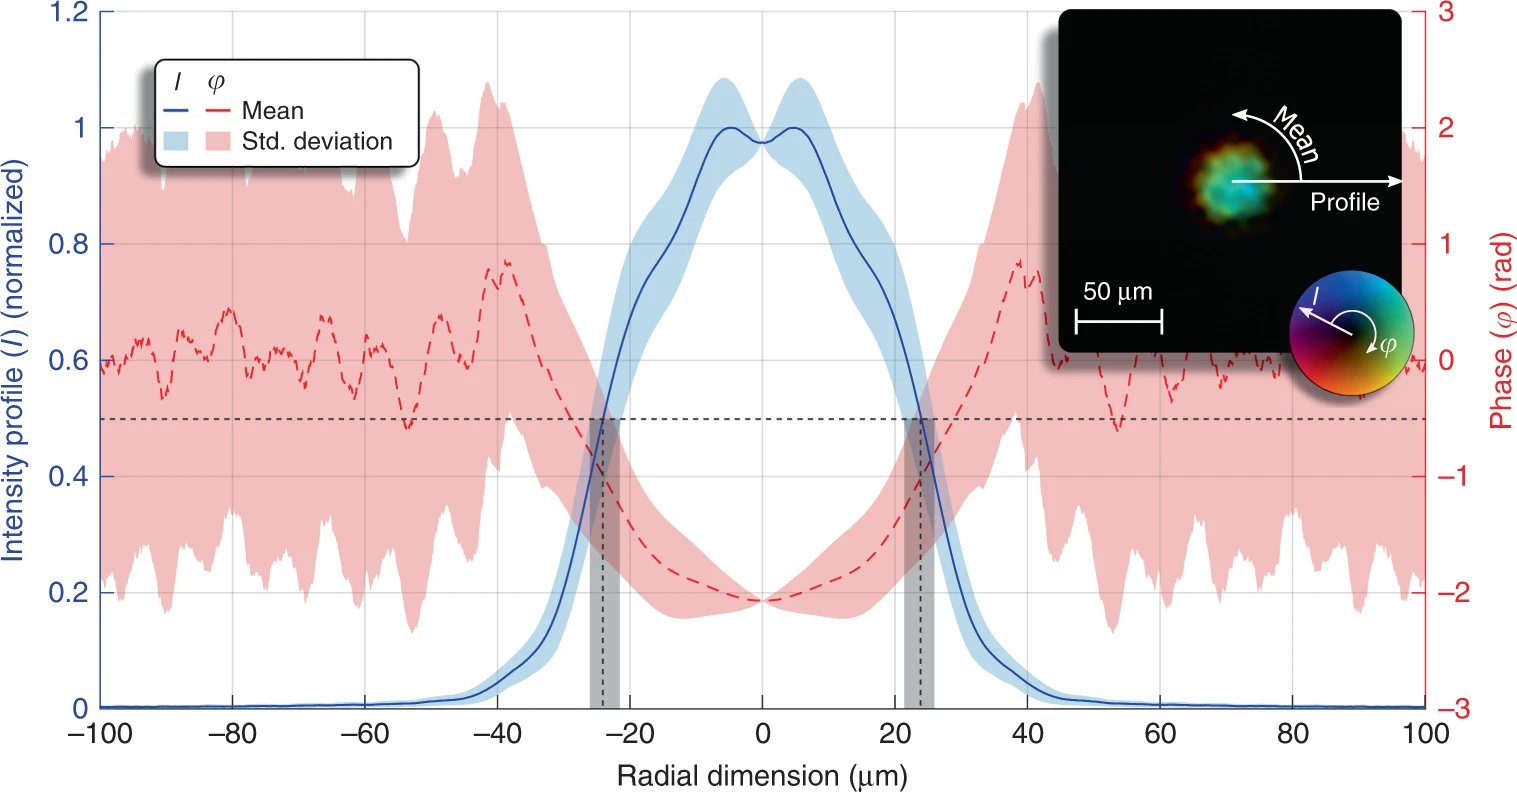
\includegraphics[width=0.8\textwidth]{Figuras/ch2_curvas_lab.png}
  \caption{Perfiles de intensidad (en rojo) y fase (en azul)\autocite{Tuitje2020} obtenidos experimentalmente en el \acrshort{loa}}
  \label{fig:4.1}
\end{figure}

Consecuentemente, para reproducir la pérdida de intensidad en dirección axial, es necesario emplear un ancho del canal con \ce{Kr^{8+}} decreciente en esta misma dirección. A medida que el láser de bombeo \acrshort{nir} viaja a través del canal de plasma, disminuye la intensidad durante su propagación por el medio activo, perdiendo capacidad para generar el ión amplificador \ce{Kr^{8+}} (responsable del efecto láser) y formándose iones inferiores, como \ce{Kr^{7+}}, \ce{Kr^{6+}}, etc. Cuando la semilla alcanza mayores longitudes del canal, la presencia del ión termina reduciéndose a franjas más estrechas ---como muestra la Figura \ref{fig:4.2}---, disminuyendo la amplificación \acrshort{sxrl} obtenida en dirección radial y axial.

Analizando estos elementos, para modelar este ancho variable del canal se propone utilizar una curva logística o sigmoide descrita por la expresión 
\begin{equation}\label{eq:4.0}
  r_{L}(z) = r_{i,min} + \frac{r_{i,max}-r_{i,min}}{1+\eu^{k_{i}(z-z_{0i})}},
\end{equation}
dependiente principalmente de cuatro parámetros: $r_{i,max}$ (valor máximo de la curva), $r_{i,min}$ (valor mínimo de la curva), $k_{i}$ (tasa de decrecimiento o pendiente de la curva) y $z_{0i}$ (coordenada $z$ donde la curva toma su valor medio).

\begin{figure}[htbp]
  \centering
  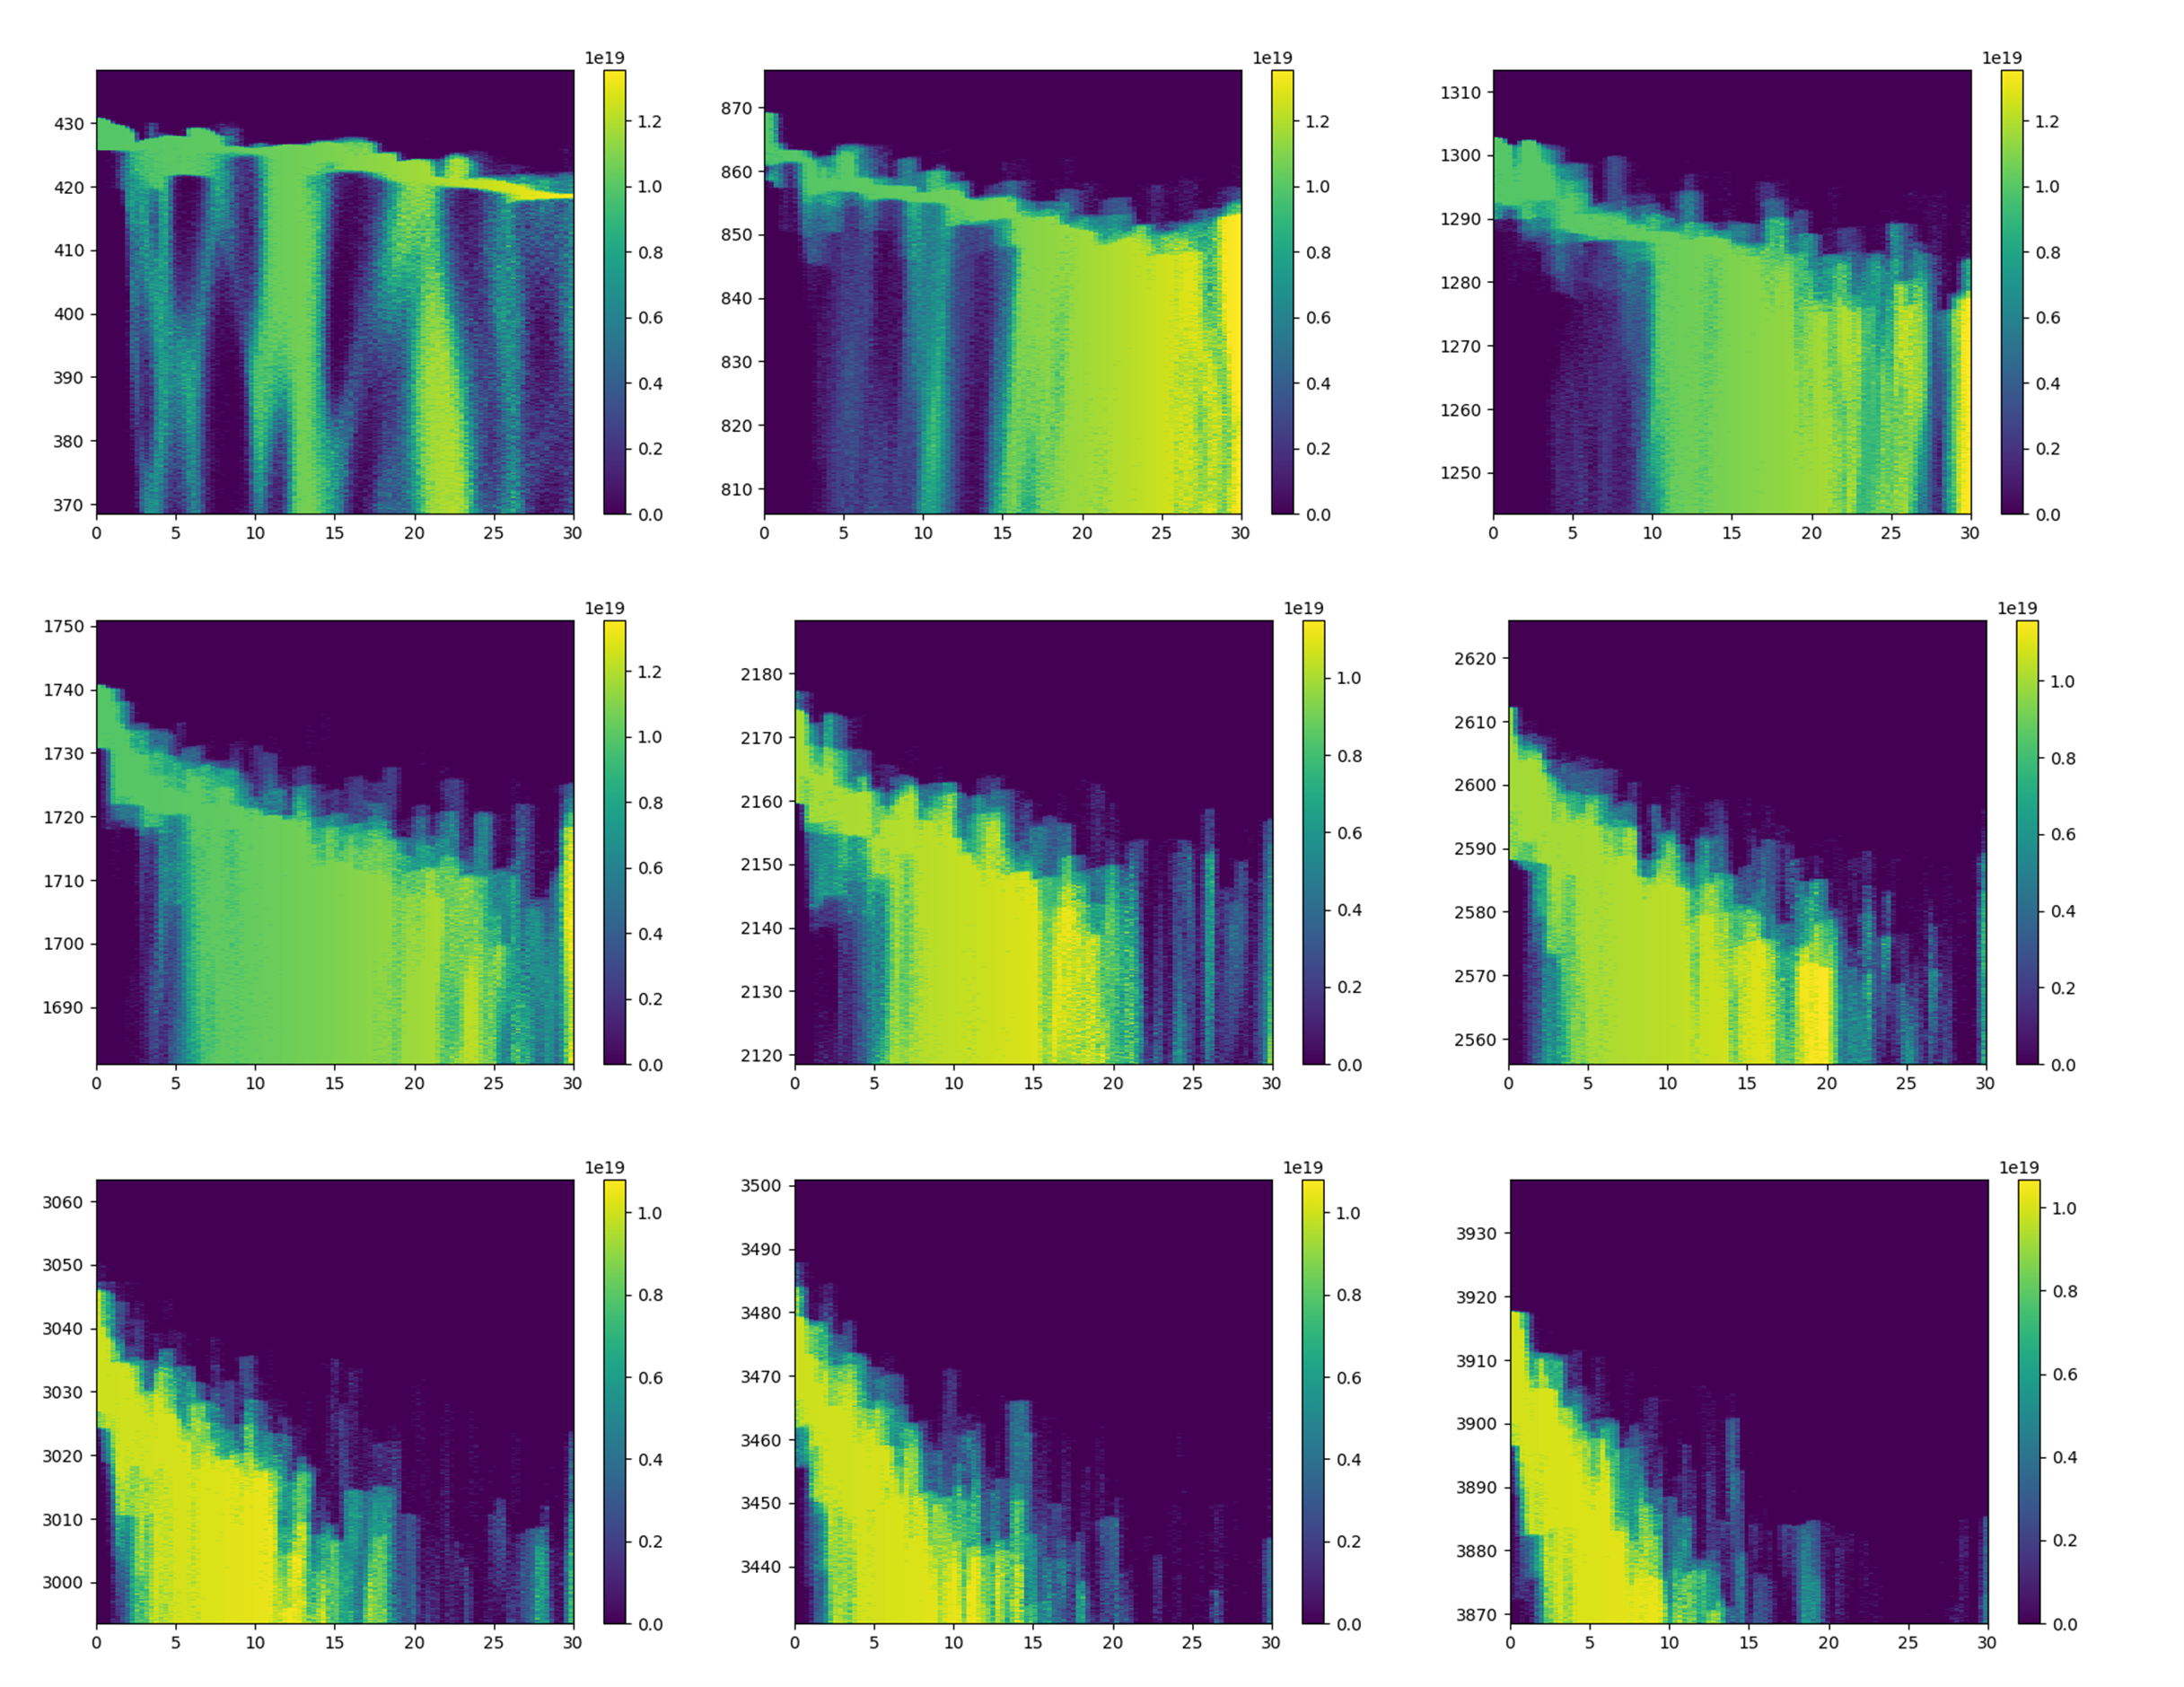
\includegraphics[width=0.8\textwidth]{Figuras/ch4_ionkr8.png}
  \caption{Densidad de \ce{Kr^{8+}} en \unit{cm^{-3}} para diferentes secciones transversales del canal de plasma. El eje horizontal representa la coordenada radial $r$ (\unit{µm}) y el eje vertical la coordenada axial $z$ (\unit{µm})}
  \label{fig:4.2}
\end{figure}

Estos parámetros permiten dar la forma deseada a la región de abundancia con \ce{Kr^{8+}}, controlando la velocidad de la transición entre el valor máximo y mínimo en dirección radial mediante $k_{i}$, además de la posición de la columna de plasma donde comienza el descenso con $z_{0i}$. En este trabajo, el canal tiene un radio de \qty{5}{mm}, por lo que los parámetros $r_{i,min}$ y $r_{i,max}$ introducidos tomarán valores alternantes entre \qty{0}{mm} y \qty{5}{mm}. Siguiendo este patrón, es posible comparar la amplificación final obtenida con ancho constante y variable.

Por ejemplo, las Figuras \ref{fig:ch4_sigma} y \ref{fig:ch4_sigmb} representan gráficamente dos sigmoides para un ancho del canal variable y constante, respectivamente. La región variable utiliza como valores de los parámetros $r_{i,min}=\qty{0}{\um}$, $r_{i,max}=\qty{5}{\um}$, $k_{i}=\qty{4000}{m^{-1}}$ y $z_{0i}=\qty{3.5}{mm}$. En cambio, la región constante emplea los parámetros $r_{i,min}=r_{i,max}=\qty{5}{\um}$, estableciendo una frontera de \ce{Kr^{8+}} con un radio constante de $r_{L}(z)=\qty{5}{\um}$ y eliminando la sigmoide, de acuerdo con la ecuación \eqref{eq:4.0}.

\begin{figure}[htbp]
  \centering
  \begin{subcaptionblock}{.4\textwidth}
    \centering
    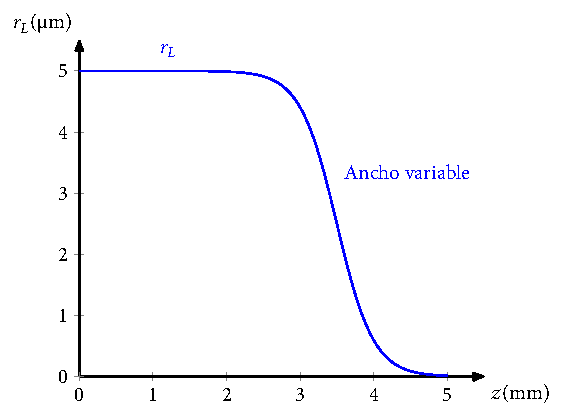
\includegraphics[width=\textwidth]{Figuras/ch4_ejsigm1.pdf}
    \caption{Región de abundancia de \ce{Kr^{8+}} variable}\label{fig:ch4_sigma}
  \end{subcaptionblock}
  \begin{subcaptionblock}{.4\textwidth}
    \centering
    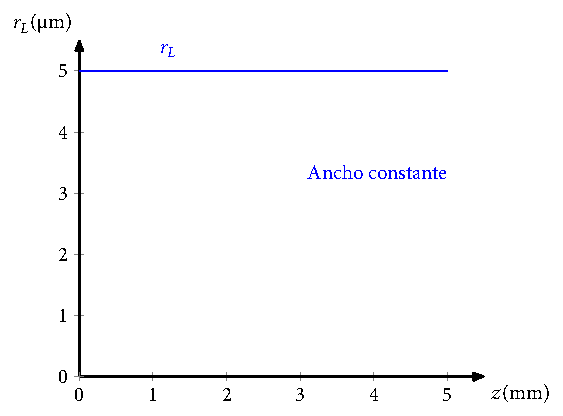
\includegraphics[width=\textwidth]{Figuras/ch4_ejsigm2.pdf}
    \caption{Región de abundancia de \ce{Kr^{8+}} constante}\label{fig:ch4_sigmb}
  \end{subcaptionblock}
   \caption{Ejemplos de sigmoides para anchos del canal variable y constante. El eje de abscisas representa la longitud recorrida en milímetros $z$ (\unit{mm}) y el eje de ordenadas el radio de abundancia de \ce{Kr^{8+}} en micrómetros $r$ (\unit{\um})}
   \label{fig:4.3}
\end{figure}

Después de encontrar la forma del perfil con presencia del ión amplificador ---una función sigmoide--- deseada, la siguiente etapa del proceso consiste en escribir un programa auxiliar para experimentar con los parámetros, antes de decidir las simulaciones a ejecutar e implementar la curva logística en el código Dagon. De esta forma, el código \ref{cod:4.1} ---escrito en MATLAB--- permite realizar esta labor a través de un pequeño programa llamado \texttt{c\_logistica.m}, visualizando las curvas logísticas y el efecto de variar los distintos parámetros.

Además, este programa también incorpora una segunda curva logística. Ambas sigmoides sustituyen un radio del canal con \ce{Kr^{8+}} constante por un vector que depende de la longitud de propagación $z$. En conjunto, habilitando las dos funciones pueden visualizarse las fronteras interna (meseta) y externa (falda) de la región de abundancia del ión, destinadas a controlar el perfil radial de intensidad completamente, estudiado durante la próxima sección \S\ref{sec:4.2}.

\begin{listing}[htbp]
  \caption{Programa auxiliar de MATLAB para representar sigmoides.}
  \inputminted[firstline=1, lastline=38]{matlab}{Programas/c_logistica.m}
  \label{cod:4.1}
\end{listing}

Dentro de la estructura del código Dagon, escrito en FORTRAN, las propiedades y dinámica del plasma se han implementado en el fichero \texttt{plasma3D.f03} y, en su interior, la subrutina dedicada a definir las densidades de iones y electrones del plasma es \texttt{fillplasma}. Cuando las simulaciones finalizan, un segundo programa auxiliar \texttt{hdf\_save\_Ok.py} recopila los datos obtenidos y los escribe en un fichero \texttt{.hdf} mediante un vínculo simbólico entre la carpeta de la simulación y el programa de Python. Por último, un tercer programa \texttt{computePhaseIntegrated.m} de Octave carga el fichero \texttt{.hdf} y representa los perfiles de intensidad y fase a través de otro vínculo simbólico con la carpeta de la simulación.

La sintaxis de FORTRAN y la estructura empleada en \texttt{plasma3D.f03} es muy diferente a la estructura del código \ref{cod:4.1}, diseñado para realizar pruebas con los parámetros de las sigmoides. Con el objetivo de evitar posibles problemas, la segunda etapa del proceso consiste en escribir dos programas separados consistentes en una función \texttt{f\_sigmoide.m} y \texttt{d\_kripton.m} similares en estructura a la utilizada en Dagon, aunque la sintaxis de ambos lenguajes de programación son distintos. 

El primer programa, mostrado en el código \ref{cod:4.2}, es una función que recibe como argumentos los parámetros de las sigmoides que delimitan la región de abundancia y las representa visualmente, mientras que el segundo programa, mostrado en el código \ref{cod:4.3}, está destinado a declarar todos los parámetros que aparecen en la densidad de \ce{Kr^{8+}} (ecuación \eqref{eq:3.19a} de densidad de \ce{Kr^{8+}}) y hacer una llamada a la función \texttt{f\_sigmoide.m} para terminar de representar el perfil de densidad.

\begin{listing}[htbp]
  \caption{Programa auxiliar de MATLAB para recibir los parámetros de la sigmoide.}
  \inputminted[firstline=1, lastline=27]{matlab}{Programas/f_sigmoide.m}
  \label{cod:4.2}
\end{listing}

\begin{longlisting}
  \caption{Programa auxiliar de MATLAB para representar el perfil de densidad de \ce{Kr^{8+}}.}
  \inputminted[firstline=1, lastline=66]{matlab}{Programas/d_kripton.m}
  \label{cod:4.3}
\end{longlisting}

Empleando esta pareja de programas, terminan las dos primeras etapas de construcción del perfil de densidad de iones \ce{Kr^{8+}}, siendo posible realizar una comparación entre las imágenes obtenidas a partir de los experimentos del \acrshort{loa} (después del postprocesamiento de los resultados) y los códigos de las simulaciones. Las Figuras \ref{fig:ch4_krmatlab} y \ref{fig:ch4_krloa} muestran gráficamente la distribución tridimensional de \ce{Kr^{8+}} obtenida mediante MATLAB y en el laboratorio\autocite{Tuitje2020}, respectivamente. Estas gráficas representan en el eje de ordenadas la densidad de \ce{Kr^{8+}} normalizada a la unidad (en MATLAB, Figura \ref{fig:ch4_krmatlab}) y como un porcentaje de la densidad de neutros de la preforma de plasma (en el experimento, Figura \ref{fig:ch4_krloa}), respectivamente. 

A pesar de que ambas imágenes difieren en un factor de escala, debido a los ejes de ordenadas escogidos, la geometría (la forma del perfil de densidad) de la columna de plasma en el momento de la inyección del \acrshort{hoh} es reproducida adecuadamente mediante los códigos \ref{cod:4.2} y \ref{cod:4.3}, apareciendo las distintas regiones características de los iones. 

Una disminución de densidad ---valle central de la intensidad y fase--- para los radios más pequeños del canal aparece formado (sobreionización de la columna producida por la alta intensidad del pulso \acrshort{nir} para radios menores), así como la gran depresión en la zona central producida por los efectos de la focalización del haz \acrshort{nir} de bombeo durante el guiado. Los máximos locales o \enquote{picos} también aparecen representados, seguidos por un rápido descenso de la concentración de \ce{Kr^{8+}} hacia radios creciente del canal, originándose una \enquote{falda} que completa el perfil.

\begin{figure}[htbp]
  \centering
  \begin{subcaptionblock}{.4\textwidth}
    \centering
    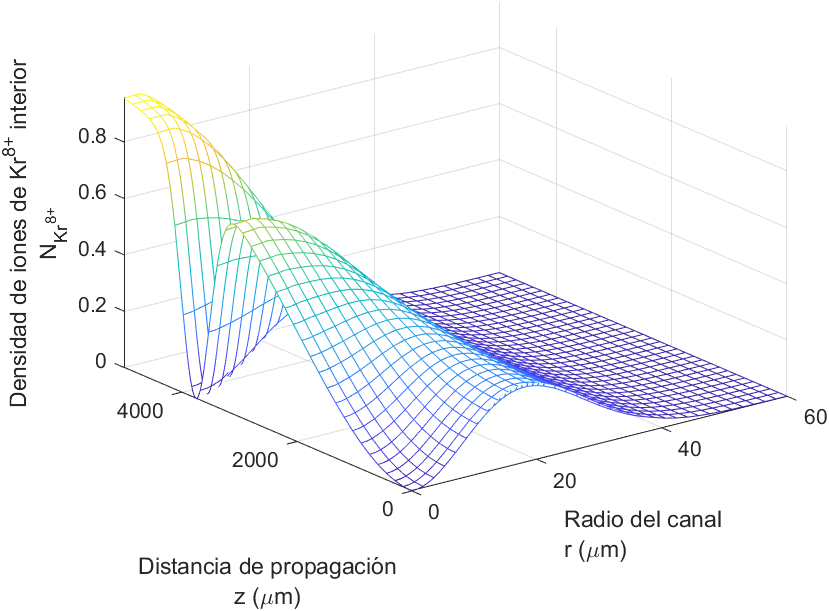
\includegraphics[width=\textwidth]{Figuras/ch4_krMatlab.png}
    \caption{Representación de la densidad de \ce{Kr^{8+}} en MATLAB}\label{fig:ch4_krmatlab}
  \end{subcaptionblock}
  \begin{subcaptionblock}{.4\textwidth}
    \centering
    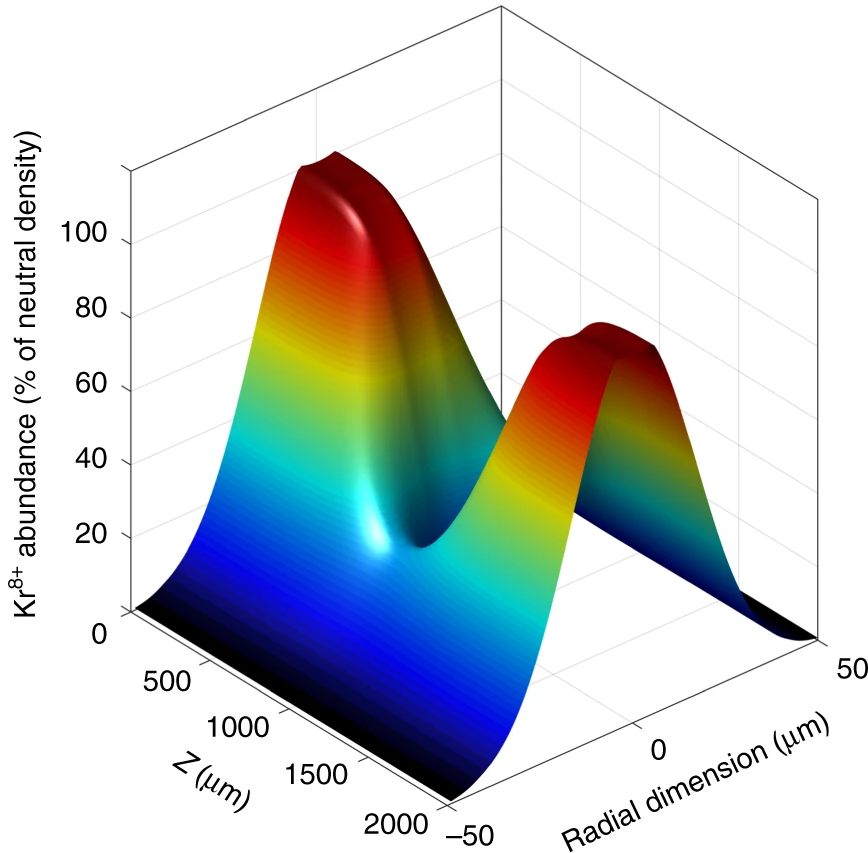
\includegraphics[width=0.8\textwidth]{Figuras/ch4_krLOA.png}
    \caption{Representación de la densidad de \ce{Kr^{8+}} experimental\autocite{Tuitje2020}}\label{fig:ch4_krloa}
  \end{subcaptionblock}
  \caption{Comparativa del perfil de densidad de \ce{Kr^{8+}} obtenido mediante MATLAB y el postprocesamiento de los resultados del experimento\autocite{Tuitje2020}. Los ejes horizontales representan la longitud de propagación en micrómetros $z$ (\unit{\um}) y la coordenada radial en micrómetros $r$ (\unit{\um}).}
  \label{fig:4.4}
\end{figure}

Por último, la tercera etapa termina la secuencia trasladando la sintaxis utilizada hasta el código Dagon en FORTRAN, fijando los parámetros de las simulaciones que mantienen sus valores a lo largo del proceso, es decir, durante la totalidad del proyecto. FORTRAN es un lenguaje de bajo nivel ---en comparación con MATLAB, en este caso---, y es recomendable consultar bibliografía actualizada\autocite{Metcalf2018} para adaptar entre programas escritos en lenguajes distintos. La materialización en Dagon aparece en el código \ref{cod:4.4}, que incluye un pequeño fragmento del programa \texttt{plasma3D.f03} donde aparecen los parámetros principales de la primera sigmoide, la distribución del canal de plasma y el cálculo de los perfiles de densidad electrónica e iónica.

\begin{longlisting}
  \caption{Fragmento del código Dagon dedicado a introducir la primera sigmoide.}
  \inputminted[firstline=1, lastline=77]{fortran}{Programas/plasma3Ds.f90}
  \label{cod:4.4}
\end{longlisting}

Los resultados de ejecutar los diferentes grupos de simulaciones, reflejados en las imágenes obtenidas después del postprocesado, y analizadas en las siguientes secciones, permitieron confirmar la adecuación del código comparando los perfiles radiales de intensidad y fase. De este modo, finaliza el proceso de introducción de la primera sigmoide en Dagon, necesaria para la modelización de la región de abundancia de \ce{Kr^{8+}}. 

En la Tabla \ref{tab:4.1}, aparecen recogidos todos los parámetros introducidos en Dagon (relativos al canal de plasma) cuyos valores se mantienen constantes y, por tanto, no constituyen objeto de estudio ni modificación durante este capítulo \S\ref{cap:4}. En cambio, las próximas tablas empleadas recogen los parámetros variados constantemente durante el proyecto, permitiendo la comparación y consulta de los cambios realizados. 

\begin{table}[htpb]
  \centering
  \caption{Parámetros fijos de las simulaciones.}
  \label{tab:4.1}
  \begin{tabular}{SSSSSSS}
  \toprule
  {$r_{c}$ (\unit{\um})} & {$r_{0}$ (\unit{\um})} & {$r_{v}$ (\unit{\um})} & {$\sigma_{z}$ (\unit{mm})} & {$\sigma_{r}$ (\unit{\um})} & {\texttt{z0\_fac}} & {\texttt{rlion\_z0} (\unit{\um})} \\ 
  \midrule
  38  & 80  & 90  & 0.25  & 15  & 0.15  & 40    \\
  38  & 80  & 90  & 0.25  & 15  & 0.15  & 40    \\
  38  & 80  & 90  & 0.25  & 15  & 0.15  & 40    \\
  38  & 80  & 90  & 0.25  & 15  & 0.15  & 40    \\
  38  & 80  & 90  & 0.25  & 15  & 0.15  & 40    \\
  38  & 80  & 90  & 0.25  & 15  & 0.15  & 40    \\ 
  \bottomrule
  \end{tabular}
\end{table}

\subsection{Variando el parámetro $r_{i,min}$}\label{sec:4.1.1}
El inicio de las simulaciones comienza fijando $r_{i,max}=\qty{5}{µm}$ y haciendo variar el parámetro $r_{i,min}$ entre \qty{0}{µm} y \qty{5}{µm} de micrómetro en micrómetro. De esta manera, pueden observarse cuáles son los efectos de $r_{i,min}$ en los perfiles de intensidad y fase, es decir, modificando el radio mínimo con presencia de \ce{Kr^{8+}} de la columna de plasma. También es posible entender esta aproximación como la frontera del canal que contiene \ce{Kr^{8+}} cuando $\lim_{z \to \infty}r_{L}(z)$. La Figura \ref{fig:4.5} muestra las sigmoides utilizadas junto a su $r_{i,min}$ correspondiente.

La transición brusca entre ambos radios mínimo y máxima es conseguida utilizando una magnitud para la pendiente de las curvas logísticas elevada de $k_{i}=\qty{50e6}{m^{-1}}$, centrando el cambio rápido de la frontera en la coordenada $z=\qty{3.8}{mm}$. Este método permite simular regiones de abundancia formadas por dos anchos del canal constantes, asociadas a dos partes de la columna de plasma separadas cuando la longitud $z=\qty{3.8}{mm}$ es alcanzada. 

El primer caso $r_{i,min}=r_{i,max}=\qty{5}{µm}$ representa un ancho del canal constante de \qty{5}{µm} en todo el canal de plasma, mientras que $r_{i,min}=\qty{0}{µm}$ y $r_{i,max}=\qty{5}{µm}$ consiste en una frontera de \qty{5}{µm} durante los primeros $z=\qty{3.8}{mm}$ de recorrido, seguidos de una desaparición súbita de \ce{Kr^{8+}}. Ambas situaciones encierran la máxima y mínima amplificación obtenible, respectivamente.

\begin{figure}[htbp]
  \centering
  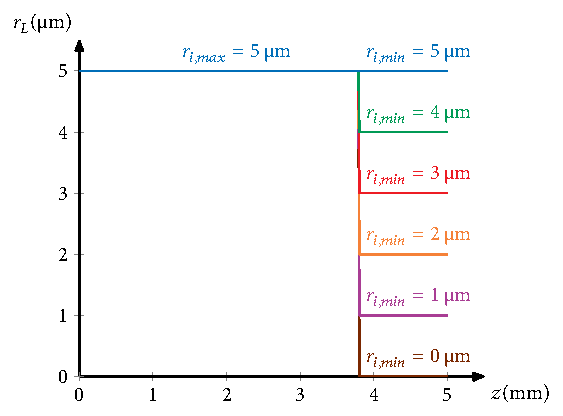
\includegraphics[width=0.5\textwidth]{Figuras/ch4_sigm_rmin.pdf}
  \caption{Sigmoides introducidas con $r_{i,min}\in[\qty{0}{µm},\qty{5}{µm}]$ y $r_{i,max}=\qty{5}{µm}$, manteniendo los valores de los parámetros $k_{i}=\qty{50e6}{m^{-1}}$ y $z_{0i}=\qty{3.8}{mm}$.}
  \label{fig:4.5}
\end{figure}

Cuando el ión amplificador queda reducido a una fracción del plasma (caso $r_{i,min}=\qty{0}{µm}$ y $r_{i,max}=\qty{5}{µm}$), la ganancia total conseguida por el pulso \acrshort{sxrl} disminuye. En la Figura \ref{fig:4.6}, se recogen los perfiles radiales de intensidad y fase obtenidos durante las simulaciones, mostrando la ausencia del valle de intensidad necesario para un buen acuerdo con el experimento, aunque también aparecen la meseta central de intensidad y los picos en el perfil de fase. El eje horizontal representa la coordenada radial en micrómetros, mientras que los ejes verticales representan la intensidad en \unit{W/cm^2} (ver Figura \ref{fig:ch4_int01}) y la fase en radianes (ver Figura \ref{fig:ch4_fs01}) del pulso.

\begin{figure}[htbp]
  \centering
  \begin{subcaptionblock}{.4\textwidth}
    \centering
    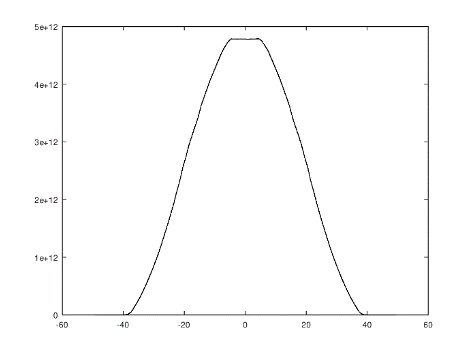
\includegraphics[width=\textwidth]{Figuras/ch4_int01.png}
    \caption{Perfil radial de intensidad (\unit{W/cm^2}) frente al radio (\unit{µm})}\label{fig:ch4_int01}
  \end{subcaptionblock}
  \begin{subcaptionblock}{.4\textwidth}
    \centering
    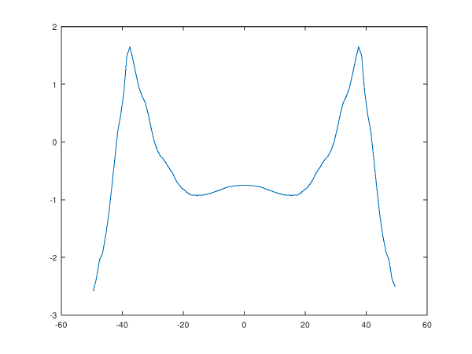
\includegraphics[width=\textwidth]{Figuras/ch4_fs01.png}
    \caption{Perfil radial de fase (\unit{rad}) frente al radio (\unit{µm})}\label{fig:ch4_fs01}
  \end{subcaptionblock}
   \caption{Distribución radial de intensidad--fase con $r_{i,min}=\qty{0}{µm}$ y $r_{i,max}=\qty{5}{µm}$, manteniendo los valores de los parámetros $k_{i}=\qty{50e6}{m^{-1}}$ y $z_{0i}=\qty{3.8}{mm}$.}
   \label{fig:4.6}
\end{figure}

Además, la superposición de las imágenes con los perfiles obtenidos en el laboratorio, permite comparar los resultados observar las diferencias. La Figura \ref{fig:4.7} demuestra el mal acuerdo entre simulación y experimento, principalmente debido a la ausencia del valle central de intensidad. Por otra parte, el perfil de fase tiene un cambio de concavidad en la zona central ($r=\qty{0}{µm}$) inexistente en el experimento, aunque el ajuste entre los máximos y mínimos locales es aceptable.

También es importante resaltar el cambio de pendiente de la curva de intensidad experimental producido en $r=\qty{17}{µm}$ aproximadamente, provocando una diferencia entre la falda de las curvas en la simulación ---donde no existe un cambio de tendencia--- y en el experimento. Naturalmente, esto es debido a la utilización de una única sigmoide, destinada a reproducir la parte superior o meseta, pero incapaz de controlar el perfil completo, sugiriendo una posible segunda sigmoide.

\begin{figure}[htbp]
  \centering
  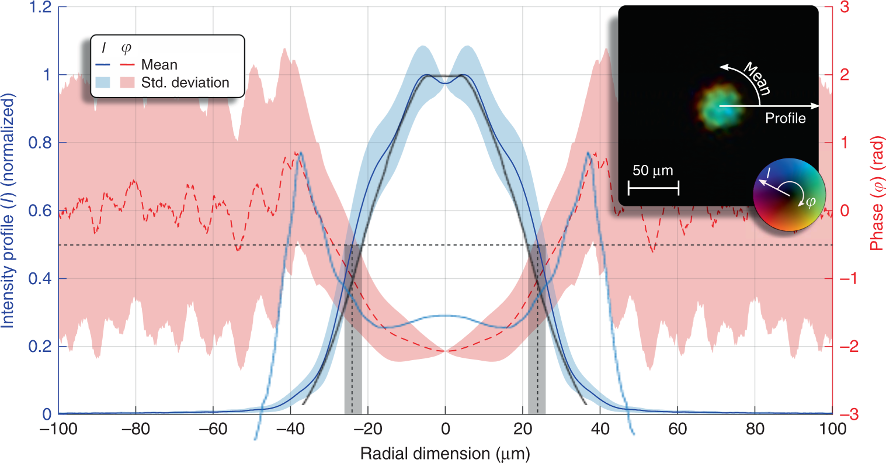
\includegraphics[width=0.75\textwidth]{Figuras/ch4_cmp01.png}
  \caption{Comparación entre los perfiles radiales de intensidad--fase con $r_{i,min}=\qty{0}{µm}$ y $r_{i,max}=\qty{5}{µm}$, manteniendo los valores de los parámetros $k_{i}=\qty{50e6}{m^{-1}}$ y $z_{0i}=\qty{3.8}{mm}$; y el experimento.}
  \label{fig:4.7}
\end{figure}

Sin embargo, cuando el ión amplificador ocupa completamente la columna de plasma (caso $r_{i,min}=r_{i,max}=\qty{5}{µm}$), la amplificación de la semilla \acrshort{hoh} es máxima. Ahora, la Figura \ref{fig:4.8} muestra la formación del valle de intensidad buscado, consiguiendo una adaptación precisa de la meseta del perfil, como aparece en la Figura \ref{fig:4.9}. De todo el grupo de simulaciones realizadas en esta sección \S\ref{sec:4.1.1} (consultar el anexo \S\ref{anx:1}), solamente presenta el valle correctamente formado este caso. La argumentación más plausible que explica este fenómeno sugiere que la intensidad necesaria para conseguir la sobreionización del valle tiene que ser la mayor posible, cubriendo el canal de plasma con \ce{Kr^{8+}} en su totalidad.

\begin{figure}[htbp]
  \centering
  \begin{subcaptionblock}{.4\textwidth}
    \centering
    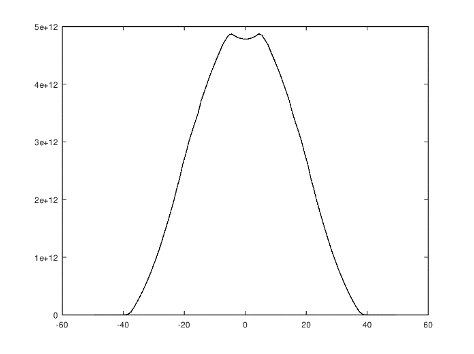
\includegraphics[width=\textwidth]{Figuras/ch4_int05.png}
    \caption{Perfil radial de intensidad (\unit{W/cm^2}) frente al radio (\unit{µm})}\label{fig:ch4_int05}
  \end{subcaptionblock}
  \begin{subcaptionblock}{.4\textwidth}
    \centering
    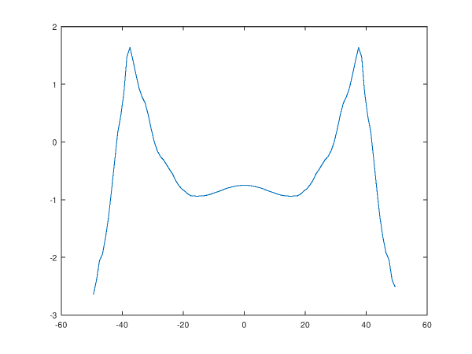
\includegraphics[width=\textwidth]{Figuras/ch4_fs05.png}
    \caption{Perfil radial de fase (\unit{rad}) frente al radio (\unit{µm})}\label{fig:ch4_fs05}
  \end{subcaptionblock}
   \caption{Distribución radial de intensidad--fase con $r_{i,min}=r_{i,max}=\qty{5}{µm}$, manteniendo los valores de los parámetros $k_{i}=\qty{50e6}{m^{-1}}$ y $z_{0i}=\qty{3.8}{mm}$.}
   \label{fig:4.8}
\end{figure}

A modo de resumen, la Tabla \ref{tab:4.2} reúne los parámetros de la sigmoide y del canal de plasma modificados en la sección \S\ref{sec:4.1.1} (concretamente, la columna $r_{i,min}$, en azul), así como otros parámetros característicos que cambiarán durante las siguientes secciones del capítulo \S\ref{cap:4}. Completando la colección de parámetros utilizados ---sin mencionar anteriormente---, las cotas $z_{ion,1}$, $z_{ion,2}$ representan las posiciones iniciales (en milímetros) de la primera y segunda zona de sobreionización del canal de plasma, respectivamente.

Por ejemplo, en la sección \S\ref{sec:4.1.4}, la distancia de separación entre ambas regiones sobreionizadas es objeto de análisis, modificando su posición relativa a través del parámetro \texttt{zshift}, encargado de controlar la posición axial de la columna donde aparece el segundo pico de sobreionización.

\begin{figure}[htbp]
  \centering
  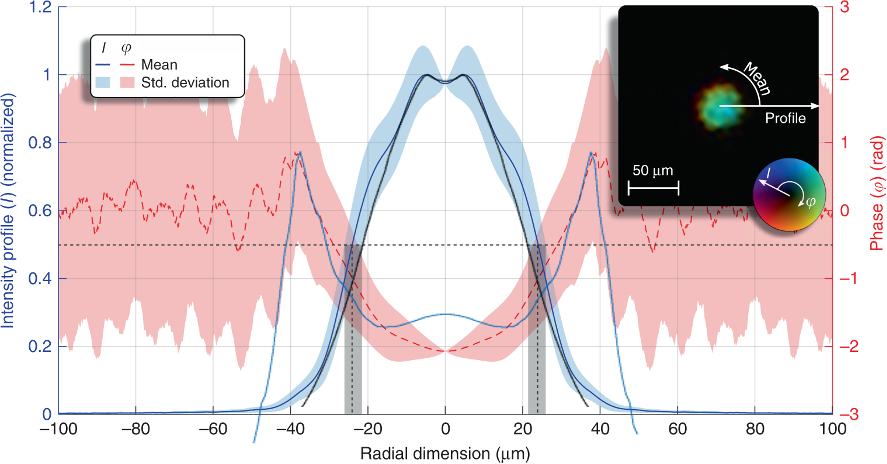
\includegraphics[width=0.75\textwidth]{Figuras/ch4_cmp05.png}
  \caption{Comparación entre los perfiles radiales de intensidad--fase con $r_{i,min}=r_{i,max}=\qty{5}{µm}$, manteniendo los valores de los parámetros $k_{i}=\qty{50e6}{m^{-1}}$ y $z_{0i}=\qty{3.8}{mm}$; y el experimento.}
  \label{fig:4.9}
\end{figure}

\begin{table}[htpb]
  \centering
  \scriptsize
  \caption{Parámetros utilizados en las simulaciones con una sigmoide, variando $r_{i,min}$ (en azul) entre \qty{0}{µm} y \qty{5}{µm}. El símbolo del \enquote{tick} señala las simulaciones con buen acuerdo.}
  \label{tab:4.2}
  \begin{tabular}{S>{\color{miazul}}SSSSSSSSS}
  \toprule
  {$r_{i,max}$ (\unit{\um})} & {$r_{i,min}$ (\unit{\um})} & {$k_{i}$ (\unit{\um^{-1}})} & {$z_{0i}$ (\unit{mm})} & {\texttt{zshift}} & {\texttt{cen\_fac}} & {$\sigma_{z0}$ (\unit{mm})} & {$\sigma_{r0}$ (\unit{\um})} & {$z_{ion,1}$ (\unit{mm})} & {$z_{ion,2}$ (\unit{mm})} \\ 
  \midrule
  5  & 0  & 50  & 3.8  & 0.75  & 0.3  & 2  & 15  & 0  & 3.75  \\
  5  & 1  & 50  & 3.8  & 0.75  & 0.3  & 2  & 15  & 0  & 3.75  \\
  5  & 2  & 50  & 3.8  & 0.75  & 0.3  & 2  & 15  & 0  & 3.75  \\
  5  & 3  & 50  & 3.8  & 0.75  & 0.3  & 2  & 15  & 0  & 3.75  \\
  5  & 4  & 50  & 3.8  & 0.75  & 0.3  & 2  & 15  & 0  & 3.75  \\
  5  & 5\checkmark  & 50  & 3.8  & 0.75  & 0.3  & 2  & 15  & 0  & 3.75  \\ 
  \bottomrule
  \end{tabular}
\end{table}

\subsection{Variando el parámetro $z_{0i}$}\label{sec:4.1.2}
Después de observar los efectos de modificar la frontera de la región, es interesante continuar las simulaciones modificando la posición del canal donde la curva logística adquiere su valor medio. A través del parámetro $z_{0i}$, la intención es responder a la pregunta: ¿Cómo afecta la posición del punto medio entre el radio mínimo $r_{i,min}$ y máximo $r_{i,max}$ de la región de abundancia a la amplificación \acrshort{xuv}?

Este conjunto de simulaciones está relacionado con la anterior sección \S\ref{sec:4.1.1}, empleando parejas de valores alternativos del radio $r_{i,min}$ de \qty{0}{µm} por un lado, y \qty{5}{µm} por otro, acompañados de una modificación paulatina ---cada paso de \qty{0.5}{mm}--- de $z_{0i}$ entre \qty{2}{mm} y \qty{3.5}{mm}. De este modo, el grupo está constituido por cuatro pares de simulaciones, cada uno de los cuales recurre a un ancho del canal constante o variable, pero con un solo valor $z_{0i}$ en común.

Siguiendo este esquema, es sencillo comparar la amplificación de la semilla \acrshort{hoh} producida por la curva logística de la Figura \ref{fig:ch4_sigm2_z0} ---idéntica al segundo caso analizado en la sección \S\ref{sec:4.1.1}---, y la conseguida con las distintas fronteras representadas en la Figura \ref{fig:ch4_sigm1_z0}. Entonces, la dirección axial del canal de plasma aparece dividida en dos tramos de distintas longitudes (el primer tramo totalmente lleno de \ce{Kr^{8+}} y el otro vacío, visto en cada sigmoide de la Figura \ref{fig:ch4_sigm1_z0}), enfrentándose a un ancho de la región de abundancia constante (visto en la sigmoide de la Figura \ref{fig:ch4_sigm2_z0}) de máxima amplificación.

A partir de la Figura \ref{fig:4.11}, es evidente que el valle y la meseta central de intensidad desaparecen, formándose un único máximo global de intensidad en $r=\qty{0}{µm}$, en desacuerdo absoluto con los resultados experimentales. En comparación con las imágenes observadas durante la anterior sección \S\ref{sec:4.1.1}, el punto medio de la sigmoide está retrasado hasta $z_{0i}=\qty{2}{mm}$, provocando la eliminación de la meseta horizontal vista en la comparación de la Figura \ref{fig:4.7}.

\begin{figure}[htbp]
  \centering
  \begin{subcaptionblock}{.4\textwidth}
    \centering
    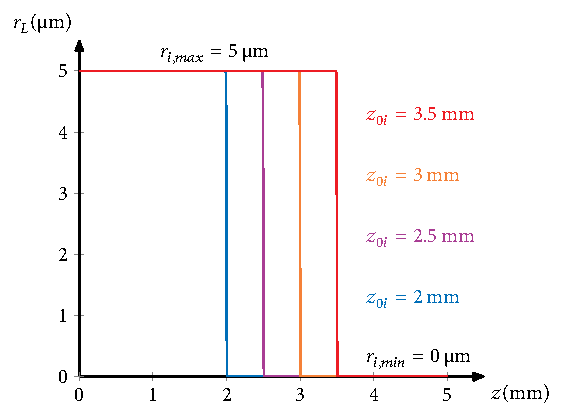
\includegraphics[width=\textwidth]{Figuras/ch4_sigm1_z0.pdf}
    \caption{Canal con $r_{i,min}=\qty{0}{µm}$ y $r_{i,max}=\qty{5}{µm}$}\label{fig:ch4_sigm1_z0}
  \end{subcaptionblock}
  \begin{subcaptionblock}{.4\textwidth}
    \centering
    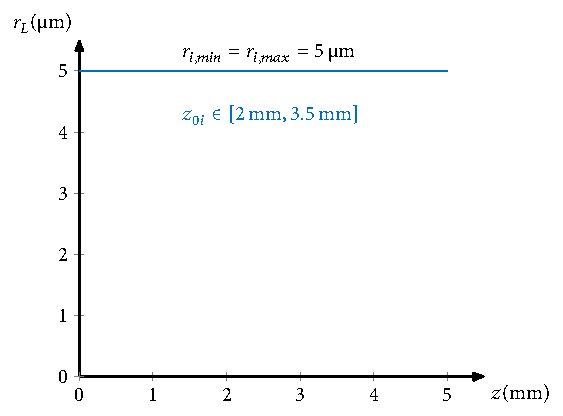
\includegraphics[width=\textwidth]{Figuras/ch4_sigm2_z0.pdf}
    \caption{Canal con $r_{i,min}=r_{i,max}=\qty{5}{µm}$}\label{fig:ch4_sigm2_z0}
  \end{subcaptionblock}
   \caption{Sigmoides introducidas con $z_{0i}\in[\qty{2}{mm},\qty{3.5}{mm}]$, manteniendo el valor del parámetro $k_{i}=\qty{50e6}{m^{-1}}$; y alternando los radios mínimo $r_{i,min}$ y máximo $r_{i,max}$ entre \qty{0}{µm} y \qty{5}{µm}.}
   \label{fig:4.10}
\end{figure}

\begin{figure}
  \centering
  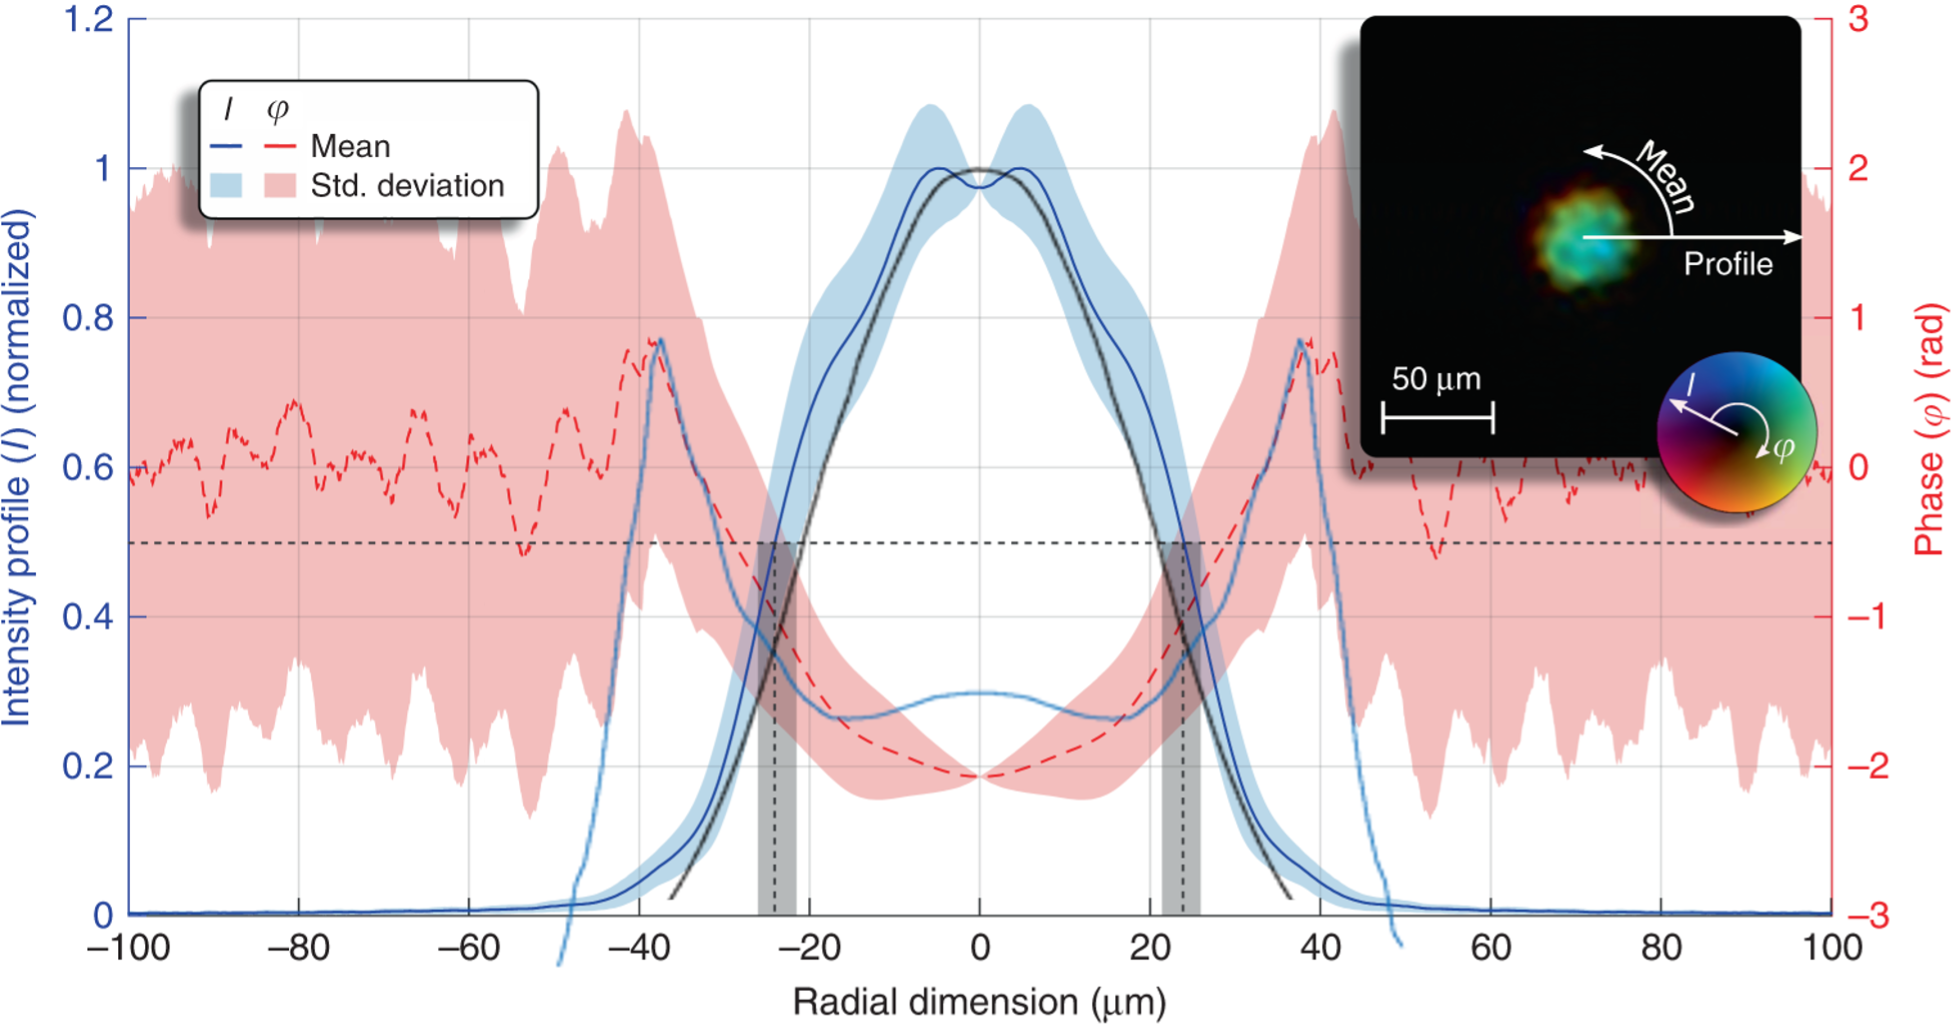
\includegraphics[width=0.75\textwidth]{Figuras/ch4_cmp11.png}
  \caption{Comparación entre los perfiles radiales de intensidad--fase con $z_{0i}=\qty{2}{mm}$, manteniendo los valores de los parámetros $r_{i,min}=\qty{0}{µm}$, $r_{i,max}=\qty{5}{µm}$ y $k_{i}=\qty{50e6}{m^{-1}}$; y el experimento.}
  \label{fig:4.11}
\end{figure}

Sin embargo, adelantando simplemente el punto medio hasta $z_{0i}=\qty{3.5}{mm}$, vuelve a formarse la meseta plana en el perfil de intensidad, como aparece en la Figura \ref{fig:4.12}. La explicación del fenómeno está en la posición de la segunda región de sobreionización del canal de plasma, en $z_{ion,2}=\qty{3.75}{mm}$, y la colocación del punto medio de la sigmoide. Cuando el comienzo de esta zona coincide aproximadamente con la coordenada $z_{0i}$, desaparecen bruscamente del canal los iones \ce{Kr^{8+}}, tal y como sucedía en el laboratorio. 

Distanciando el punto medio de la sigmoide de esta región central del canal, desplazando rígidamente la curva logística hasta coordenadas más alejadas de la zona de sobreionización (y más próximas al comienzo de la columna), la rápida disminución de \ce{Kr^{8+}} ---a partir de $z_{0i}$--- no está en consonancia con la depresión de \ce{Kr^{8+}} en la columna de plasma ---a partir de $z_{ion,2}$---, imprescindible para originar la meseta del perfil de intensidad.

Por tanto, la introducción del ancho variable del canal, mediante una sigmoide, necesariamente tiene que mantener la coherencia entre la posición de la región sobreionizada y la transición en la curva logística. En cualquier caso, el valle central no está presente, pues la concentración de \ce{Kr^{8+}} desaparece en el segundo tramo de la columna. La Tabla \ref{tab:4.3} recoge los parámetros empleados. 

\begin{figure}[htbp]
  \centering
  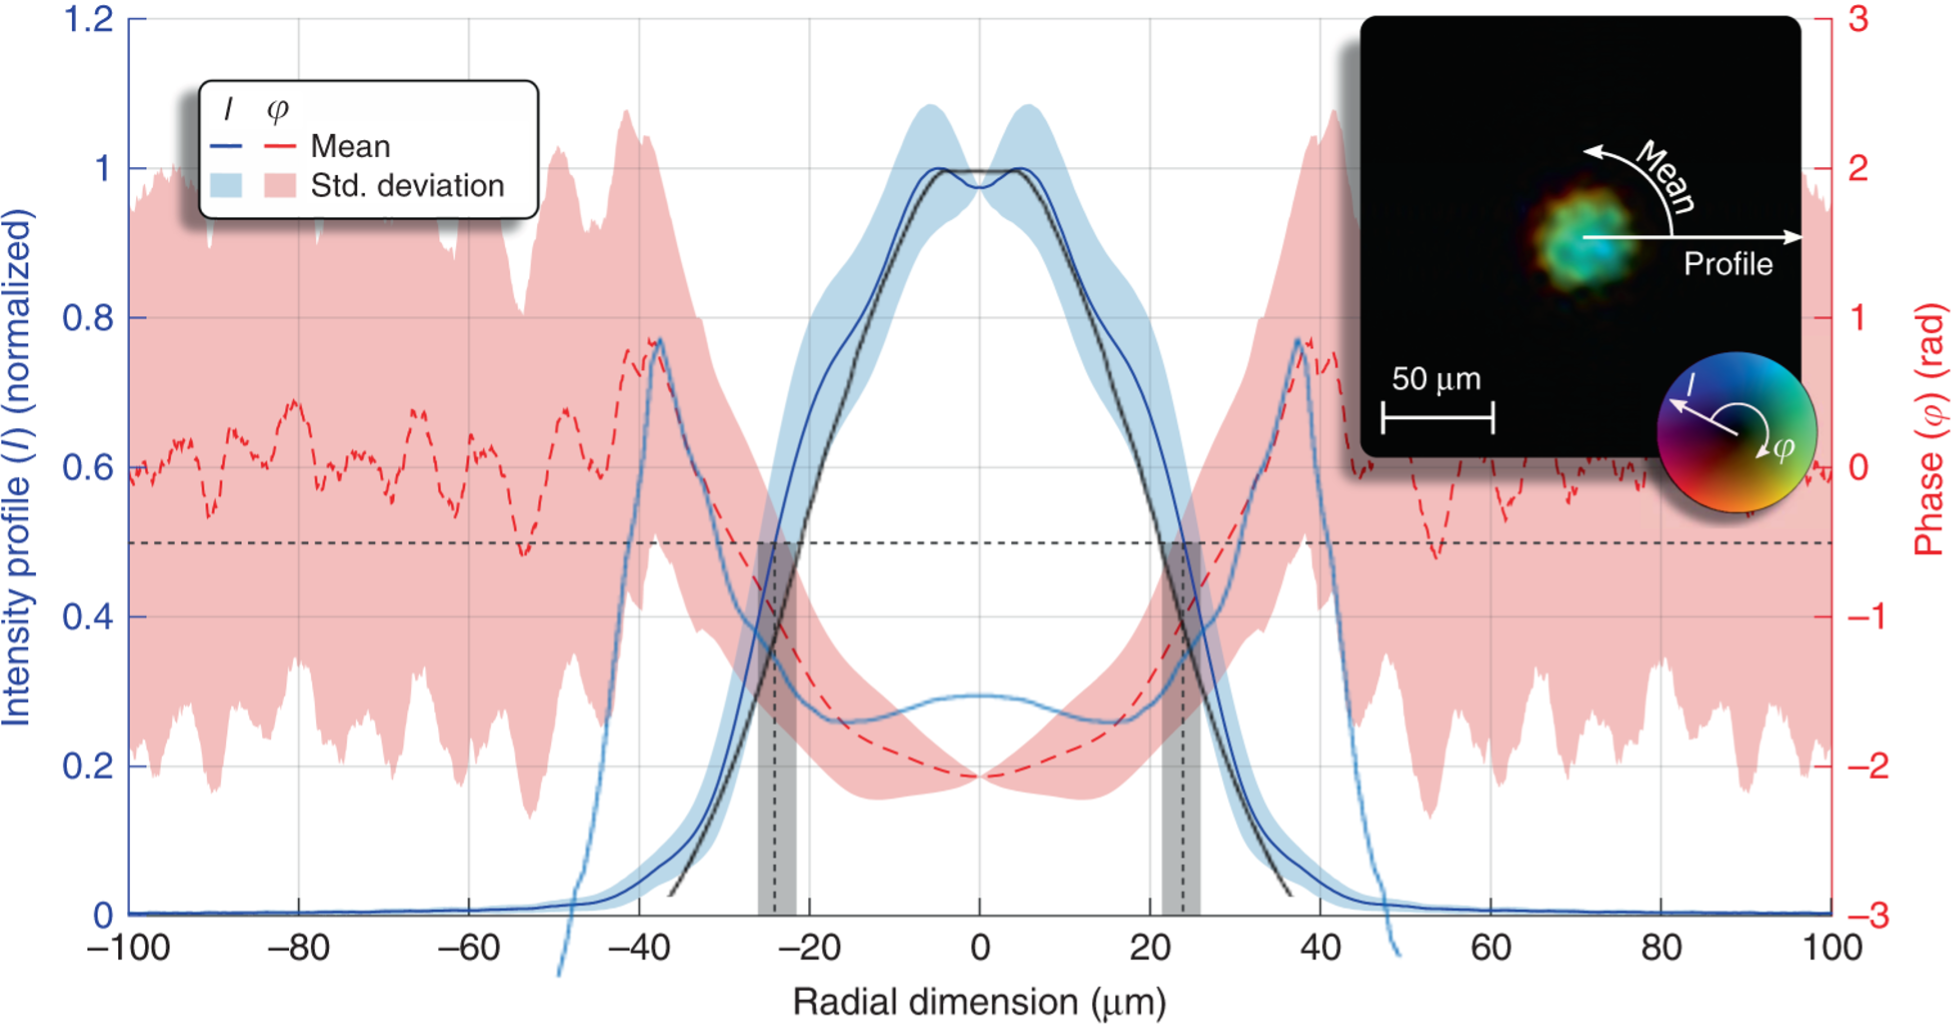
\includegraphics[width=0.75\textwidth]{Figuras/ch4_cmp12.png}
  \caption{Comparación entre los perfiles radiales de intensidad--fase con $z_{0i}=\qty{3.5}{mm}$, manteniendo los valores de los parámetros $r_{i,min}=\qty{0}{µm}$, $r_{i,max}=\qty{5}{µm}$ y  $k_{i}=\qty{50e6}{m^{-1}}$; y el experimento.}
  \label{fig:4.12}
\end{figure}

\begin{table}[htpb]
  \centering
  \scriptsize
  \caption{Parámetros utilizados en las simulaciones con una sigmoide, variando $z_{0i}$ (en azul) entre \qty{2}{mm} y \qty{3.5}{mm}; y alternando $r_{i,min}$ entre \qty{0}{µm} y \qty{5}{µm}. El símbolo del \enquote{tick} señala las simulaciones con buen acuerdo.}
  \label{tab:4.3}
  \begin{tabular}{S>{\color{miazul}}SS>{\color{miazul}}SSSSSSS}
  \toprule
  {$r_{i,max}$ (\unit{\um})} & {$r_{i,min}$ (\unit{\um})} & {$k_{i}$ (\unit{\um^{-1}})} & {$z_{0i}$ (\unit{mm})} & {\texttt{zshift}} & {\texttt{cen\_fac}} & {$\sigma_{z0}$ (\unit{mm})} & {$\sigma_{r0}$ (\unit{\um})} & {$z_{ion,1}$ (\unit{mm})} & {$z_{ion,2}$ (\unit{mm})} \\ 
  \midrule
  5  & 0  & 50  & 2  & 0.75  & 0.3  & 2  & 15  & 0  & 3.75  \\
  5  & 5 \checkmark  & 50  & 2  & 0.75  & 0.3  & 2  & 15  & 0  & 3.75  \\
  5  & 0  & 50  & 2.5  & 0.75  & 0.3  & 2  & 15  & 0  & 3.75  \\
  5  & 5 \checkmark  & 50  & 2.5  & 0.75  & 0.3  & 2  & 15  & 0  & 3.75  \\
  5  & 0  & 50  & 3  & 0.75  & 0.3  & 2  & 15  & 0  & 3.75  \\
  5  & 5 \checkmark  & 50  & 3  & 0.75  & 0.3  & 2  & 15  & 0  & 3.75  \\
  5  & 0  & 50  & 3.5  & 0.75  & 0.3  & 2  & 15  & 0  & 3.75  \\
  5  & 5 \checkmark  & 50  & 3.5  & 0.75  & 0.3  & 2  & 15  & 0  & 3.75  \\
  \bottomrule
  \end{tabular}
\end{table}

\subsection{Variando el parámetro $k_{i}$}\label{sec:4.1.3}
A continuación, motivado por las marcadas diferencias (formación o ausencia del valle central) entre los perfiles radiales de intensidad en cada pareja de simulaciones presentadas durante la sección \S\ref{sec:4.1.2}, es importante responder una nueva pregunta: ¿qué ocurre cuando la tasa de variación entre $r_{i,min}$ y $r_{i,max}$ es más suave y regular? Modificando el parámetro $k_{i}$, la pendiente de la curva logística puede adaptarse fácilmente e intentar adaptar la amplificación \acrshort{xuv} a las observaciones.

Específicamente, esta sección \S\ref{sec:4.1.3} busca regularizar la transición entre los radios máximo y mínimo del canal de plasma, utilizados anteriormente en las secciones \S\ref{sec:4.1.1} y \S\ref{sec:4.1.2}, mientras la sigmoide es desplazada simultáneamente desde $z_{0i}=\qty{2}{mm}$ hasta $z_{0i}=\qty{3.5}{mm}$, recogidos en la Tabla \ref{tab:4.4}. El esquema seguido consiste en variar ambos parámetros progresivamente, alcanzando una situación donde $r_{i,min}=\qty{0}{µm}$ exactamente en $z=\qty{5}{mm}$, es decir, el radio tiene que decaer lentamente hasta llegar al final de la columna de plasma.

Observando la superposición de la Figura \ref{fig:4.14}, se reproduce el mismo problema explicado en la sección \S\ref{sec:4.1.2}. Aunque la transición es más lenta, el punto medio $z_{0i}$ de la curva logística está demasiado alejado de la segunda zona de sobreionización del canal, de ahí que aparezca nuevamente la discrepancia en la formación de la meseta central y, por supuesto, del valle que realmente está siendo perseguido. Del mismo modo, la Figura \ref{fig:4.15} presenta una meseta en el perfil de intensidad, gracias al desplazamiento rígido de la sigmoide hacia $z_{0i}=\qty{3.5}{µm}$, muy cercana a la coordenada axial $z_{ion,2}=\qty{3.75}{µm}$ donde comienza la sobreionización central de la columna de plasma.

\begin{figure}[htbp]
  \centering
  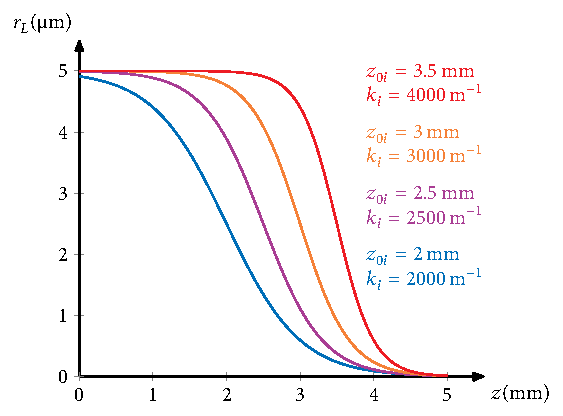
\includegraphics[width=0.5\textwidth]{Figuras/ch4_sigm_k.pdf}
  \caption{Sigmoides introducidas con $k_{i}\in[\qty{2000}{m^{-1}},\qty{4000}{m^{-1}}]$ y $z_{0i}\in[\qty{2}{mm},\qty{3.5}{mm}]$, manteniendo el valor de los parámetros $r_{i,min}=\qty{0}{µm}$ y $r_{i,max}=\qty{5}{µm}$.}
  \label{fig:4.13}
\end{figure}

\begin{figure}[htbp]
  \centering
  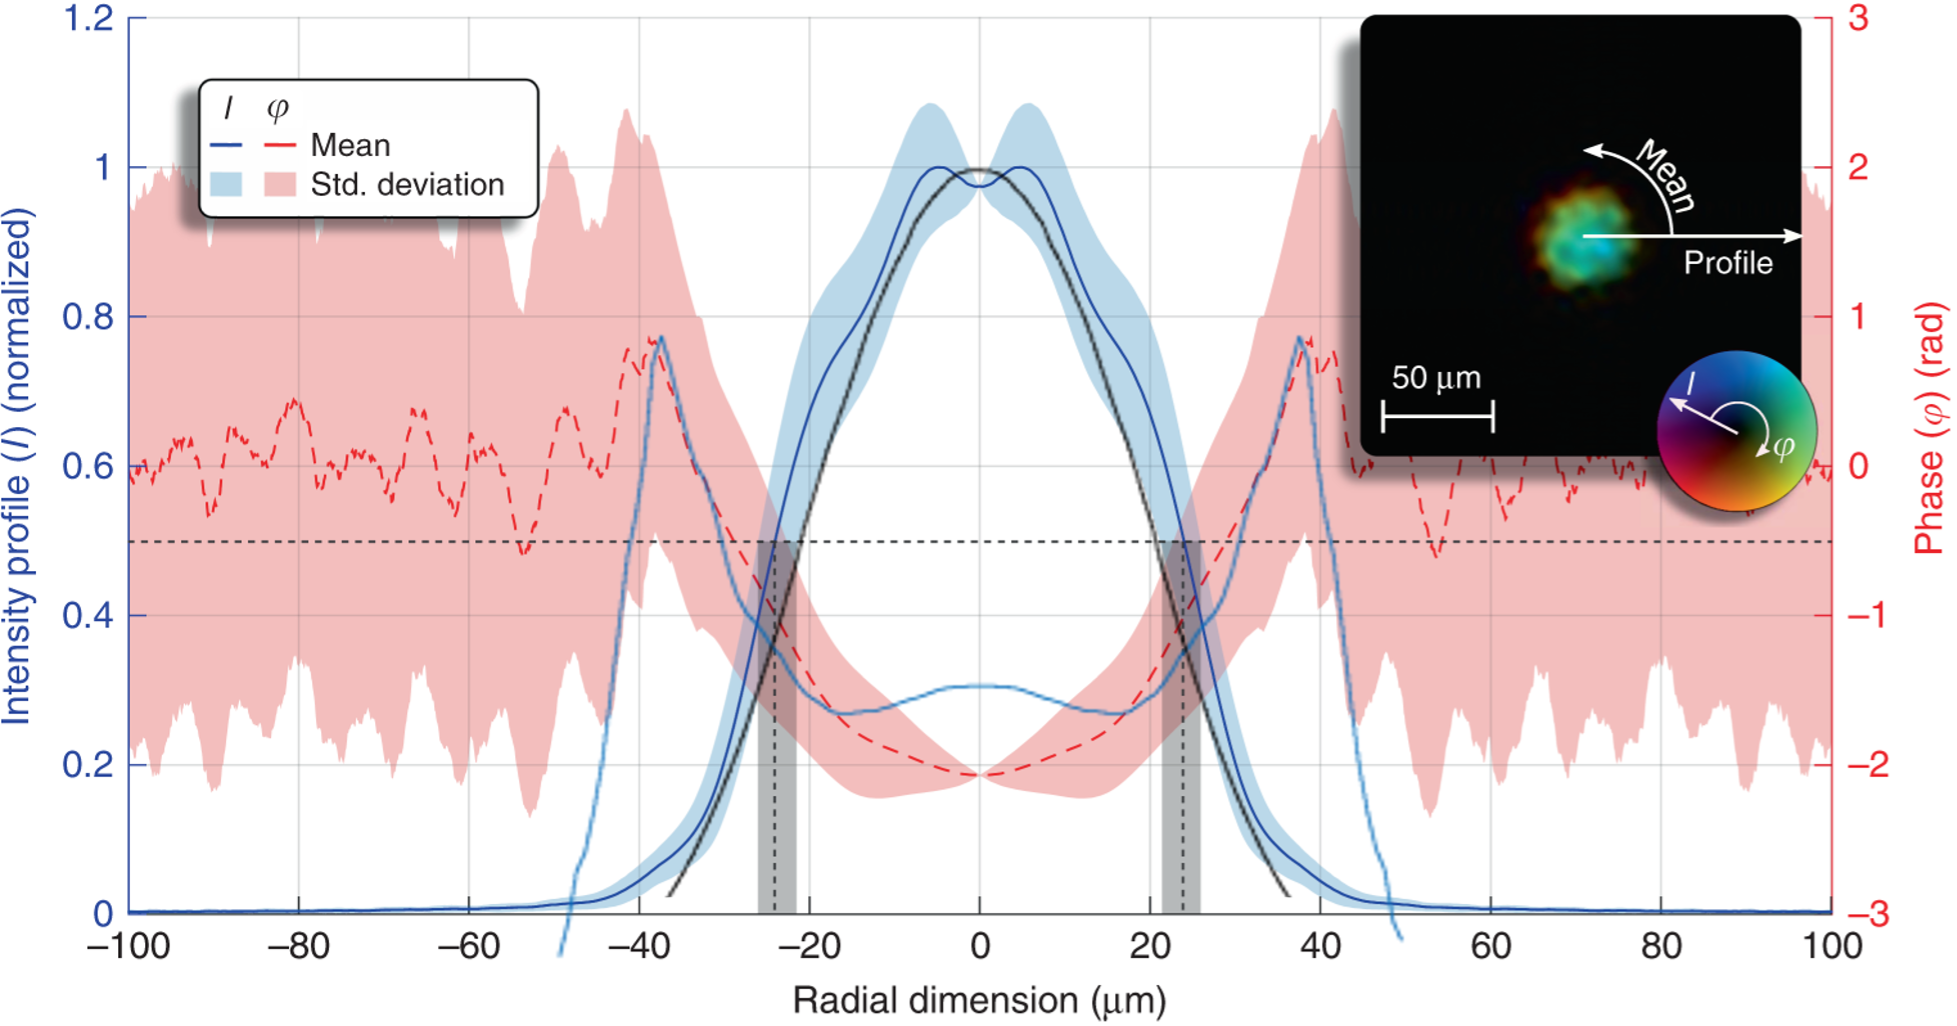
\includegraphics[width=0.7\textwidth]{Figuras/ch4_cmp21.png}
  \caption{Comparación entre los perfiles radiales de intensidad--fase con $z_{0i}=\qty{2}{mm}$ y $k_{i}=\qty{2000}{m^{-1}}$, manteniendo los valores de los parámetros $r_{i,min}=\qty{0}{µm}$ y $r_{i,max}=\qty{5}{µm}$; y el experimento.}
  \label{fig:4.14}
\end{figure}

En este punto, está claro que la curva de intensidad es imposible controlarla totalmente recurriendo a una única curva sigmoide, pues ni los valles de intensidad consiguen formarse, ni tampoco aparece el cambio de pendiente de la falda, cuando el ancho del canal introducido es variable. Utilizar un ancho constante en el canal de plasma es una hipótesis que, aunque simplifica notablemente los cálculos, no se corresponde con la distribución de \ce{Kr^{8+}} determinada experimentalmente\autocite{Tuitje2020}.

\begin{figure}[htbp]
  \centering
  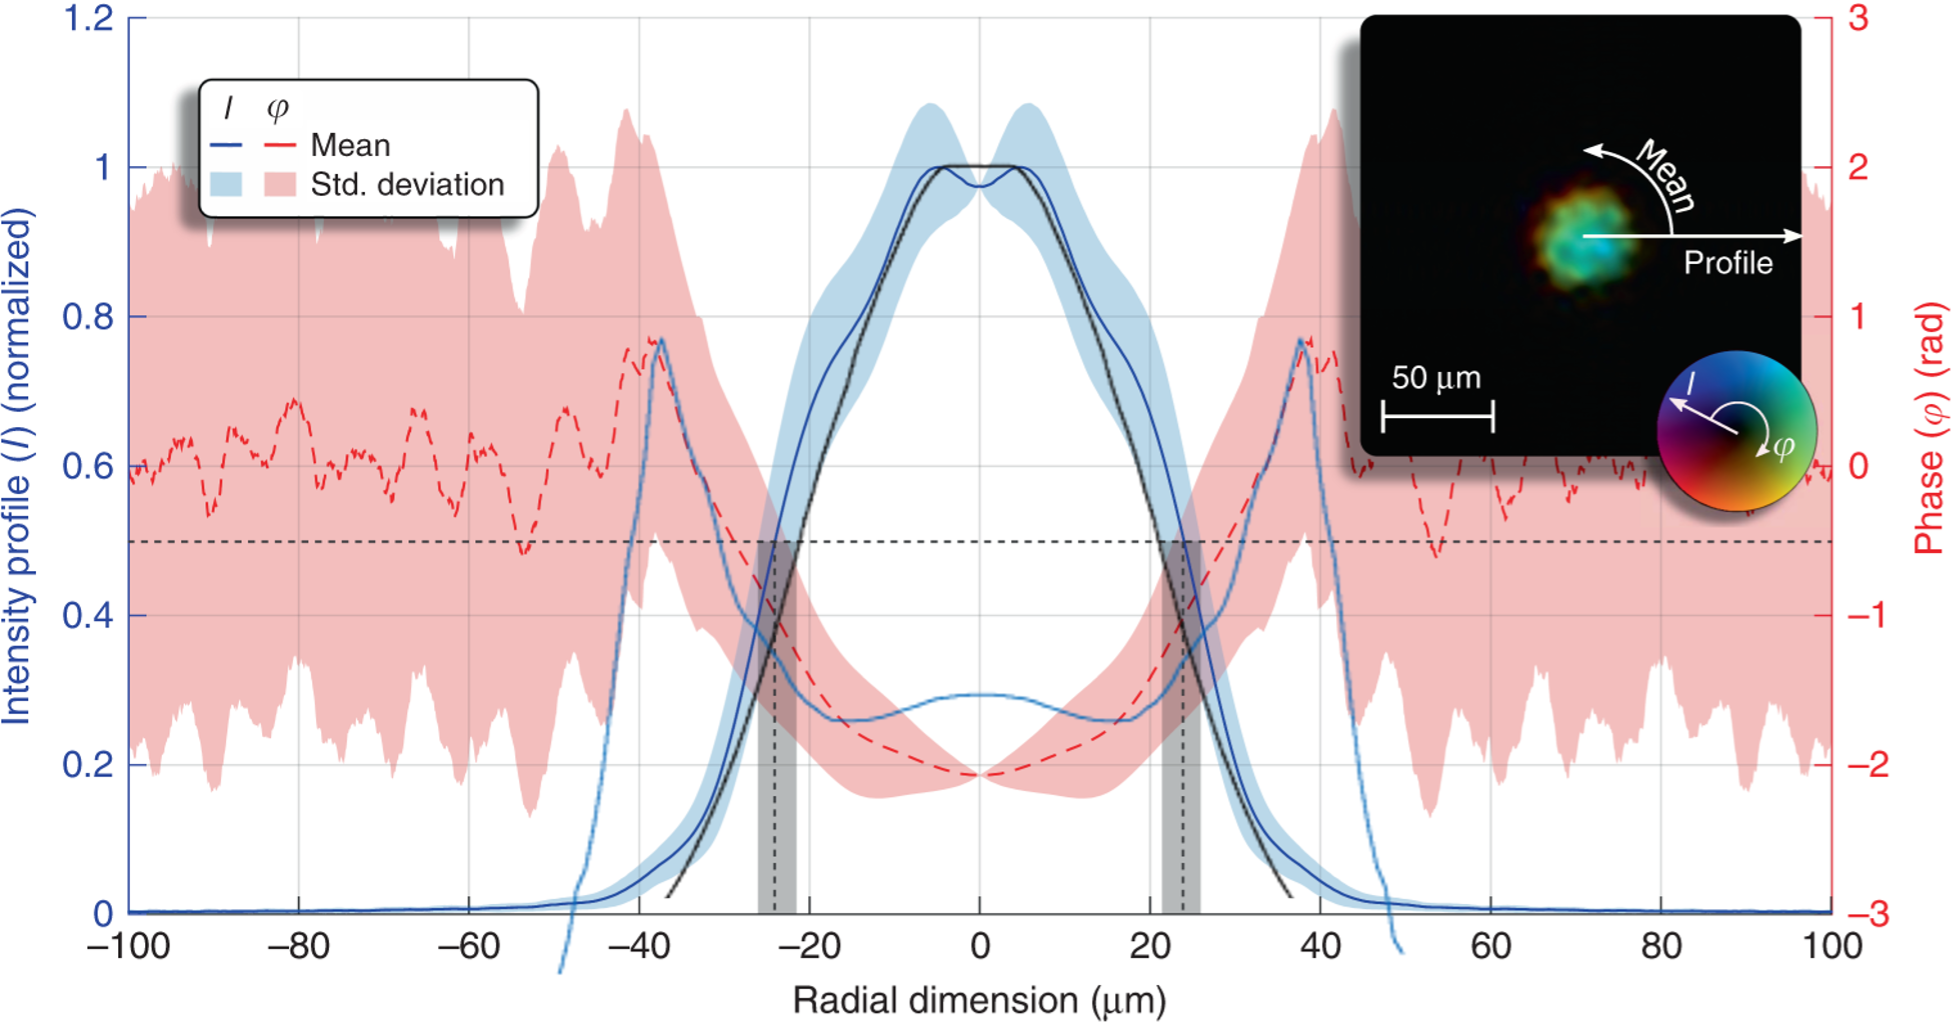
\includegraphics[width=0.68\textwidth]{Figuras/ch4_cmp22.png}
  \caption{Comparación entre los perfiles radiales de intensidad--fase con $z_{0i}=\qty{3.5}{mm}$ y $k_{i}=\qty{4000}{m^{-1}}$, manteniendo los valores de los parámetros $r_{i,min}=\qty{0}{µm}$ y $r_{i,max}=\qty{5}{µm}$; y el experimento.}
  \label{fig:4.15}
\end{figure}

Además, el perfil radial de fase mantiene la diferencia de alturas entre los máximos locales en $r=\qty{40}{µm}$ (los picos de la fase) y el mínimo local en $r=\qty{0}{µm}$, debido al cambio de concavidad producido en las simulaciones. La manera más sencilla de intentar adecuar la fase de los fotones amplificados es modificar la densidad electrónica e iónica, como en la sección \S\ref{sec:4.1.4}.

\begin{table}[htpb]
  \centering
  \scriptsize
  \caption{Parámetros utilizados en las simulaciones con una sigmoide, variando $z_{0i}$ (en azul) entre \qty{2}{mm} y \qty{3.5}{mm}; y variando $k_{i}$ entre \qty{2000}{m^{-1}} y \qty{4000}{m^{-1}}. El símbolo del \enquote{tick} señala las simulaciones con buen acuerdo.}
  \label{tab:4.4}
  \begin{tabular}{SS>{\color{miazul}}S>{\color{miazul}}SSSSSSS}
  \toprule
  {$r_{i,max}$ (\unit{\um})} & {$r_{i,min}$ (\unit{\um})} & {$k_{i}$ (\unit{\m^{-1}})} & {$z_{0i}$ (\unit{mm})} & {\texttt{zshift}} & {\texttt{cen\_fac}} & {$\sigma_{z0}$ (\unit{mm})} & {$\sigma_{r0}$ (\unit{\um})} & {$z_{ion,1}$ (\unit{mm})} & {$z_{ion,2}$ (\unit{mm})} \\ 
  \midrule
  5  & 0  & 2000  & 2  & 0.75  & 0.3  & 2  & 15  & 0  & 3.75  \\
  5  & 0  & 2500  & 2.5  & 0.75  & 0.3  & 2  & 15  & 0  & 3.75  \\
  5  & 0  & 3000  & 3  & 0.75  & 0.3  & 2  & 15  & 0  & 3.75  \\
  5  & 0  & 4000  & 3.5  & 0.75  & 0.3  & 2  & 15  & 0  & 3.75  \\
  \bottomrule
  \end{tabular}
\end{table}

\subsection{Variando el parámetro \texttt{zshift}}\label{sec:4.1.4}
Antes de iniciar el análisis de las simulaciones con dos sigmoides, es importante determinar la influencia de las zonas sobreionizadas en el perfil radial de fase. ¿Cómo afectan la extensión de las zonas sobreionizadas y su posición a este perfil de fase? El procedimiento a seguir consiste en modificar la longitud $\sigma_{z0}$ de la primera zona de sobreionización, manteniendo distancia la de separación entre el final de la primera y el comienzo de la segunda zona.  

De forma análoga a la sección \S\ref{sec:4.1.2}, este grupo de simulaciones están agrupadas en pares con y sin sigmoide, esto es, alternando anchos del canal variable y constante. El parámetro \texttt{zshift} utilizado es una fracción de la unidad que multiplica a la longitud total ($L=\qty{5}{mm}$) de la columna de plasma, situando el inicio de la segunda zona de sobreionización en $z_{ion,2}$. Por tanto, si se desea conservar la distancia (en las simulaciones realizadas durante las secciones anteriores de $z_{ion,2}-\sigma_{z0}=\qty{1.75}{mm}$) entre el final de la primera zona y el comienzo de la segunda, también es necesario cambiar la longitud $\sigma_{z0}$ de sobreionización inicial. En la Tabla \ref{tab:4.5} aparecen recogidos estos parámetros y, en la Figura \ref{fig:4.16}, los dos tipos de sigmoides insertadas.

La Figura \ref{fig:4.17} muestra el resultado obtenido cuando el ancho del canal es constante, reduciendo la longitud de la primera zona de ionización y adelantando la formación de la segunda zona en $\qty{1}{mm}$, conservando su posición relativa en la columna de plasma. 

\begin{figure}[htbp]
  \centering
  \begin{subcaptionblock}{.4\textwidth}
    \centering
    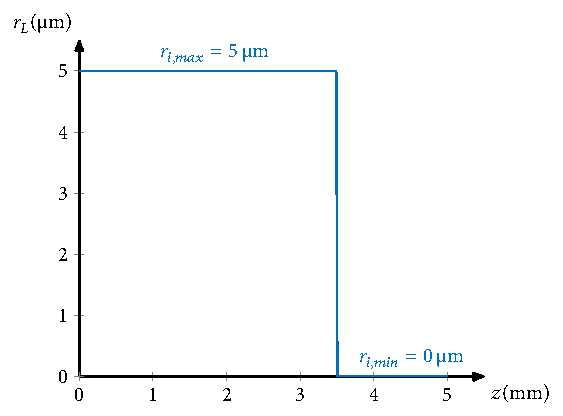
\includegraphics[width=\textwidth]{Figuras/ch4_sigm1_zs.pdf}
    \caption{Canal con $r_{i,min}=\qty{0}{µm}$ y $r_{i,max}=\qty{5}{µm}$}\label{fig:ch4_sigm1_zs}
  \end{subcaptionblock}
  \begin{subcaptionblock}{.4\textwidth}
    \centering
    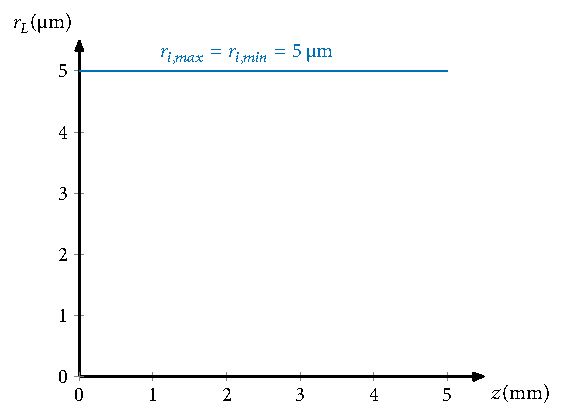
\includegraphics[width=\textwidth]{Figuras/ch4_sigm2_zs.pdf}
    \caption{Canal con $r_{i,min}=r_{i,max}=\qty{5}{µm}$}\label{fig:ch4_sigm2_zs}
  \end{subcaptionblock}
  \caption{Sigmoides introducidas con $r_{i,min}=\qty{0}{µm}$ o $r_{i,min}=\qty{5}{µm}$, y $r_{i,max}=\qty{5}{µm}$; manteniendo los valores de los parámetros $k_{i}=\qty{50e6}{m^{-1}}$ y $z_{0i}=\qty{3.5}{mm}$.}
   \label{fig:4.16}
\end{figure}

\begin{figure}[htbp]
  \centering
  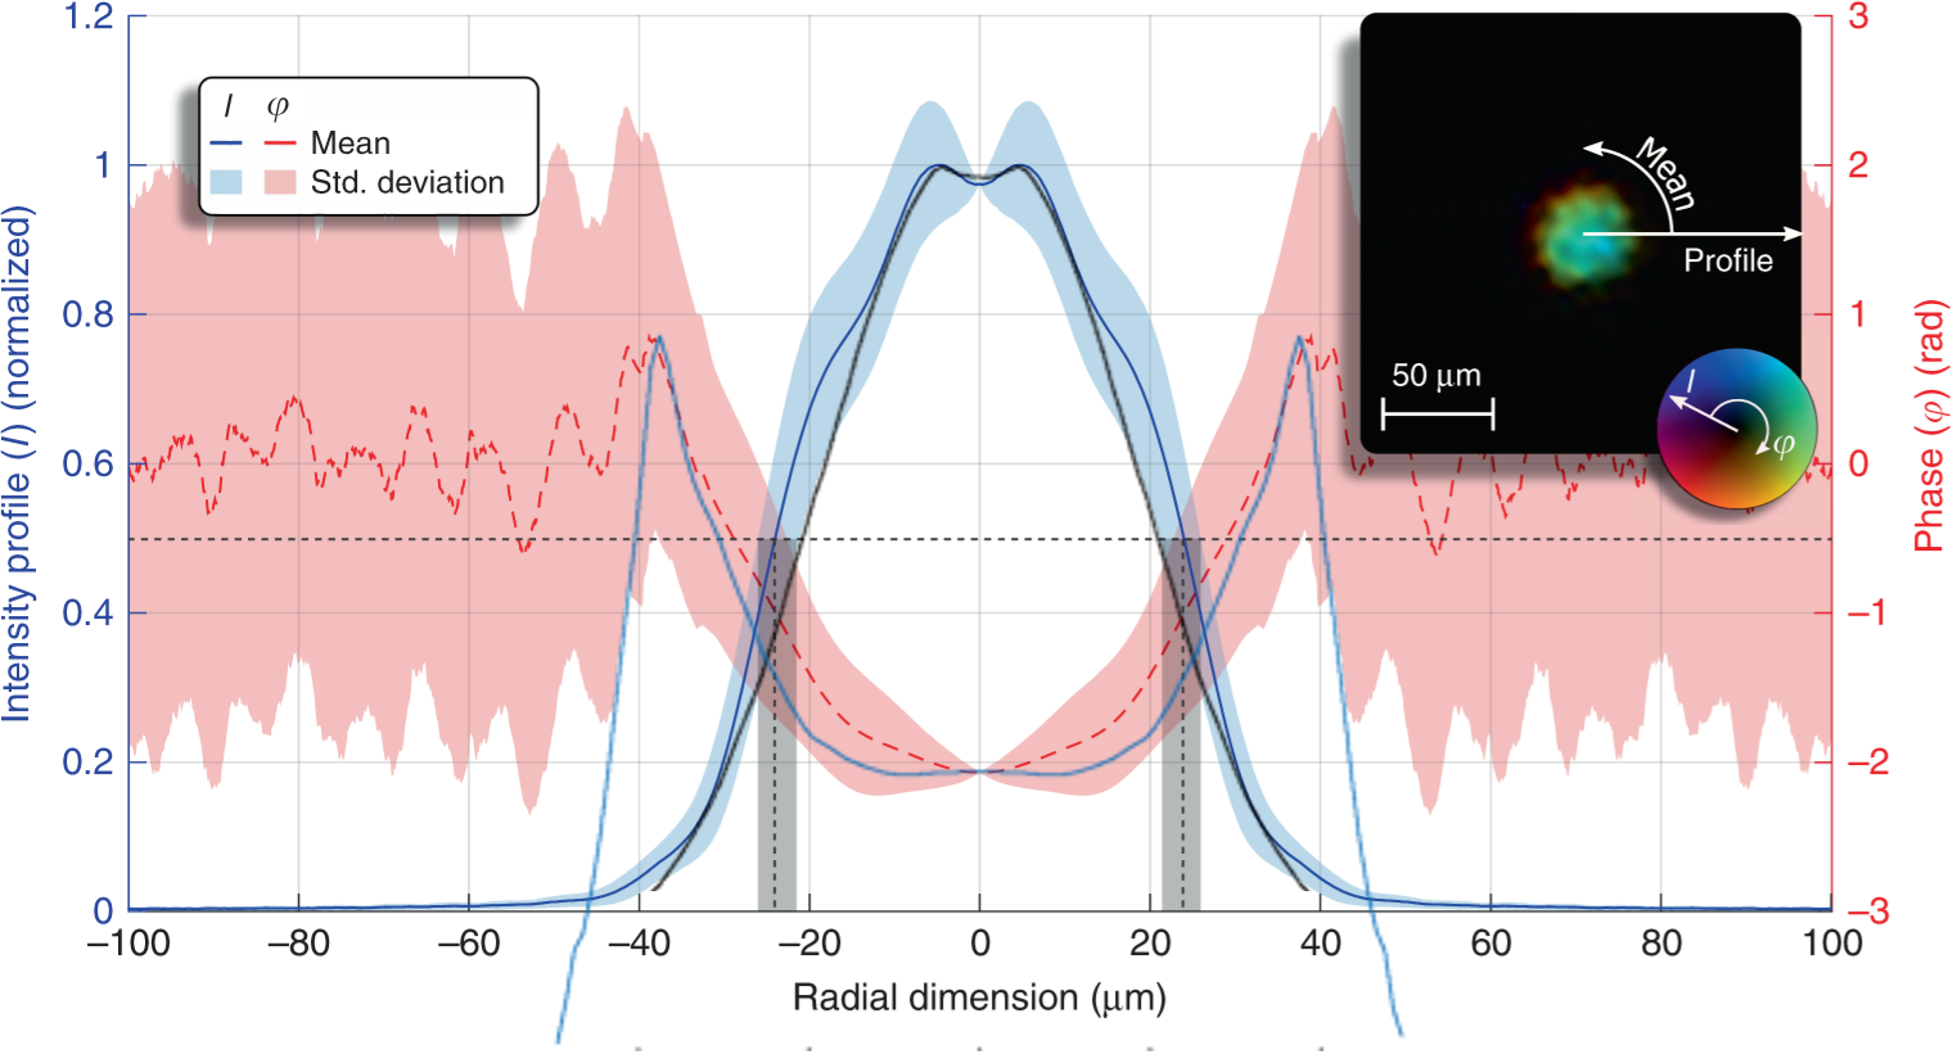
\includegraphics[width=0.7\textwidth]{Figuras/ch4_cmp31.png}
  \caption{Comparación entre los perfiles radiales de intensidad--fase con $\texttt{zshift}=0.55$, manteniendo los valores de los parámetros $r_{i,min}=r_{i,max}=\qty{5}{µm}$, $k_{i}=\qty{50e6}{m^{-1}}$ y $z_{0i}=\qty{3.5}{mm}$; y el experimento.}
  \label{fig:4.17}
\end{figure}

En este caso, existe un ajuste muy bueno en la profundidad entre el valle y los picos del perfil de fase, además de formarse el valle central de intensidad, aunque persiste ---en menor magnitud--- la concavidad detectada en la fase durante las anteriores secciones. Manteniendo un ancho constante, pero realizando estas modificaciones en las regiones sobreionizadas, el acuerdo conseguido es considerablemente preciso en ambos perfiles.

Por otra parte, la segunda simulación de la pareja ---que introduce el ancho variable---, pierde el valle de intensidad. La Figura \ref{fig:4.18} mantiene la forma conseguida del perfil de fase, ya que la posición de las franjas sobreionizadas es idéntica, pero la amplificación de la semilla a lo largo del canal es inferior, desapareciendo el valle buscado y formándose una meseta ligeramente abombada.

A medida que estas regiones sobreionizadas recuperan lentamente las posiciones y longitudes iniciales empleadas en las secciones anteriores ($\sigma_{z0}=\qty{2}{mm}$ y $z_{ion,2}=\qty{3.75}{mm}$), la profundidad del perfil de fase regresa a la discrepancia anteriormente observada, conservándose la geometría de la curva de intensidad. Si se quiere visualizar esta progresión, la secuencia completa de imágenes pueden consultarse en el anexo \S\ref{anx:1}.

\begin{figure}[htbp]
  \centering
  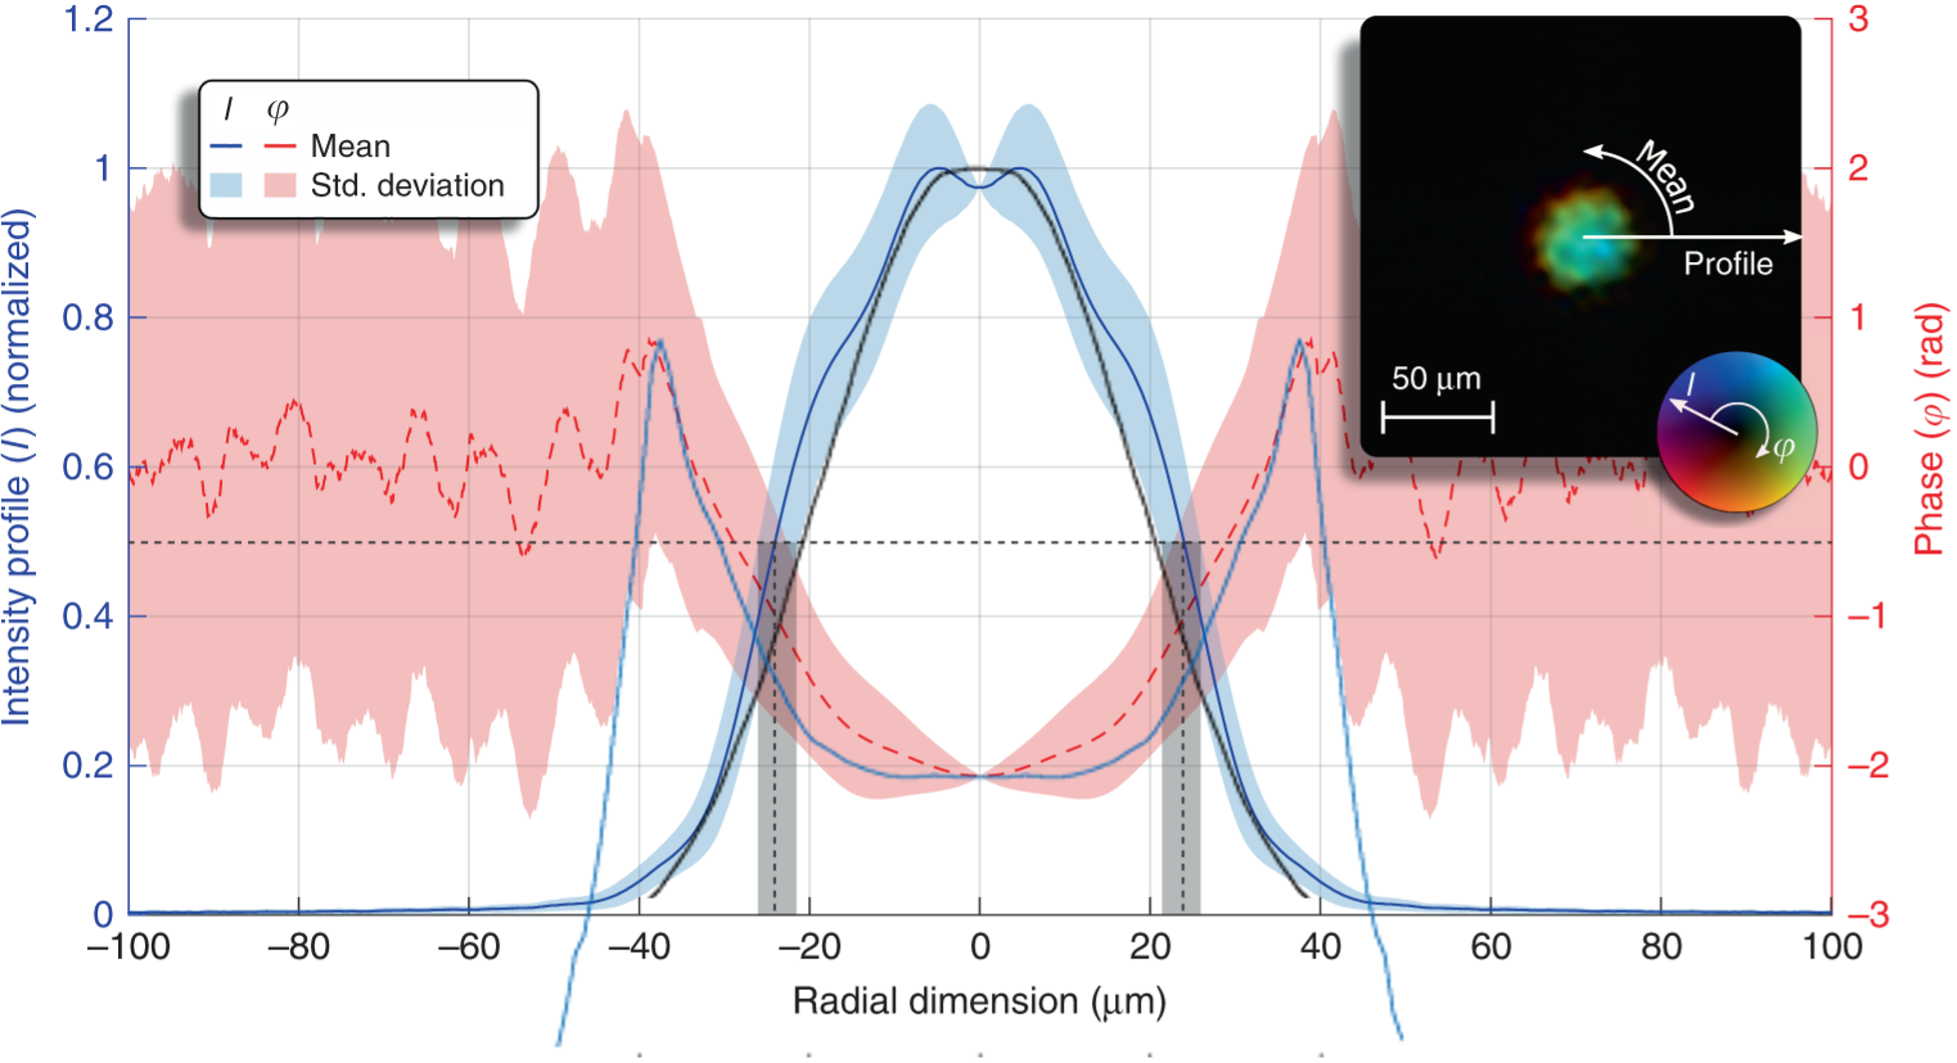
\includegraphics[width=0.75\textwidth]{Figuras/ch4_cmp32.png}
  \caption{Comparación entre los perfiles radiales de intensidad--fase con $\texttt{zshift}=0.55$, manteniendo los valores de los parámetros $r_{i,min}=\qty{0}{µm}$, $r_{i,max}=\qty{5}{µm}$, $k_{i}=\qty{50e6}{m^{-1}}$ y $z_{0i}=\qty{3.5}{mm}$; y el experimento.}
  \label{fig:4.18}
\end{figure}

Con esta sección \S\ref{sec:4.1.4} finaliza el proceso de simulaciones con una sigmoide, quedando establecidos los diferentes efectos sobre la amplificación \acrshort{xuv} conseguida, cuando la geometría y densidad del canal de plasma son modificadas. La adición de una segunda curva logística se explora durante la sección \S\ref{sec:4.2}.

\begin{table}[htpb]
  \centering
  \scriptsize
  \caption{Parámetros utilizados en las simulaciones con una sigmoide, variando \texttt{zshift} (en azul) entre \qty{0.55}{mm} y \qty{0.75}{mm}; y $\sigma_{z0}$ entre \qty{1}{mm} y \qty{2}{mm}. El símbolo del \enquote{tick} señala las simulaciones con buen acuerdo.}
  \label{tab:4.5}
  \begin{tabular}{S>{\color{miazul}}SSS>{\color{miazul}}SS>{\color{miazul}}SSS>{\color{miazul}}S}
  \toprule
  {$r_{i,max}$ (\unit{\um})} & {$r_{i,min}$ (\unit{\um})} & {$k_{i}$ (\unit{\um^{-1}})} & {$z_{0i}$ (\unit{mm})} & {\texttt{zshift}} & {\texttt{cen\_fac}} & {$\sigma_{z0}$ (\unit{mm})} & {$\sigma_{r0}$ (\unit{\um})} & {$z_{ion,1}$ (\unit{mm})} & {$z_{ion,2}$ (\unit{mm})} \\ 
  \midrule
  5  & 0  & 50  & 3.5 & 0.55  & 0.3  & 1  & 15  & 0  & 2.75  \\
  5  & 5 \checkmark  & 50  & 3.5 & 0.55  & 0.3  & 1  & 15  & 0  & 2.75  \\
  5  & 0  & 50  & 3.5 & 0.60  & 0.3  & 1.25  & 15  & 0  & 3  \\
  5  & 5 \checkmark & 50  & 3.5 & 0.60  & 0.3  & 1.25  & 15  & 0  & 3  \\
  5  & 0  & 50  & 3.5 & 0.65  & 0.3  & 1.5  & 15  & 0  & 3.25  \\
  5  & 5 \checkmark & 50  & 3.5 & 0.65  & 0.3  & 1.5  & 15  & 0  & 3.25  \\
  5  & 0  & 50  & 3.5 & 0.7  & 0.3  & 1.75  & 15  & 0  & 3.5  \\
  5  & 5 \checkmark & 50  & 3.5 & 0.7  & 0.3  & 1.75  & 15  & 0  & 3.5  \\
  5  & 0  & 50  & 3.5 & 0.75  & 0.3  & 2  & 15  & 0  & 3.75  \\
  5  & 5 \checkmark & 50  & 3.5 & 0.75  & 0.3  & 2  & 15  & 0  & 3.75  \\
  \bottomrule
  \end{tabular}
\end{table}

\section{Ajuste de la densidad de iones con dos sigmoides}\label{sec:4.2}
La introducción de una sigmoide estaba destinada a controlar la parte superior del perfil de intensidad, es decir, la formación del valle de intensidad y el ajuste entre picos y valles en el perfil de fase. Sin embargo, esta hipótesis no permite controlar los perfiles completamente, en especial la anchura de la curva de intensidad a partir de $r=\qty{17}{µm}$. Identificada la raiz del problema, esta sección \S\ref{sec:4.2} incluye una combinación de dos sigmoides $r_{L}(z)$ y $\sigma_{rL}(z)$, descritas por las ecuaciones
\begin{align}
  \label{eq:4.1a}
  r_{L}(z) &= r_{i,min} + \frac{r_{i,max}-r_{i,min}}{1+\eu^{k_{i}(z-z_{0i})}}, \\
  \label{4.1b}
  \sigma_{rL}(z) &= r_{ig,min} + \frac{r_{ig,max}-r_{ig,min}}{1+\eu^{k_{ig}(z-z_{0ig})}},
\end{align}
con $r_{ig,min}$, $r_{ig,max}$, $k_{ig}$ y $z_{0ig}$ los parámetros de la segunda sigmoide, análogos a los utilizados en la primera sigmoide. 

Para intentar adaptar el cambio de tendencia de la falda de intensidad, los siguientes apartados están centrados en modificar los parámetros de la segunda curva logística, manteniendo los parámetros de la primera sigmoide constantes. De este modo, la frontera interior con abundancia de \ce{Kr^{8+}} consiste en un único ancho variable del canal en todos los casos, mientras que la frontera exterior es modificada para determinar sus efectos sobre la curva de intensidad completa. La Figura \ref{fig:4.19} muestra las características de la primera sigmoide (en la Figura \ref{fig:ch4_ssigma}), y el ejemplo de una segunda sigmoide (en la Figura \ref{fig:ch4_ssigmb}).

Antes de comenzar el proceso de simulaciones, es necesario realizar una pequeña modificación en Dagon que incorpore esta nueva curva logística. Simplemente hay que sustituir el parámetro $\sigma_{r}=\qty{15}{µm}$ por $\sigma_{rL}(z)$ en el interior del término cociente de exponenciales que aparecía en la ecuación \eqref{eq:3.19a} para la densidad de \ce{Kr^{8+}}, de manera análoga a la sustitución que se hizo en la sección \S\ref{sec:4.1} del parámetro $r_{L0}=\qty{5}{µm}$ por $r_{L}(z)$. 

El código \ref{cod:4.5} incluye un pequeño fragmento modificado del programa \texttt{plasma3D.f03} donde aparecen los parámetros de la primera y segunda sigmoide, la distribución parabólica de especies en la preforma inicial de plasma, terminando con el cálculo de los perfiles de densidad electrónica e iónica. La variable \texttt{sig\_r} es sustituida por el vector \texttt{sig\_rig(:)} utilizado para almacenar la segunda curva logística, igual que \texttt{rlion\_cen} fue sustituido por el vector \texttt{ri(:)} que almacenaba la primera sigmoide.

\begin{figure}[htbp]
  \centering
  \begin{subcaptionblock}{.4\textwidth}
    \centering
    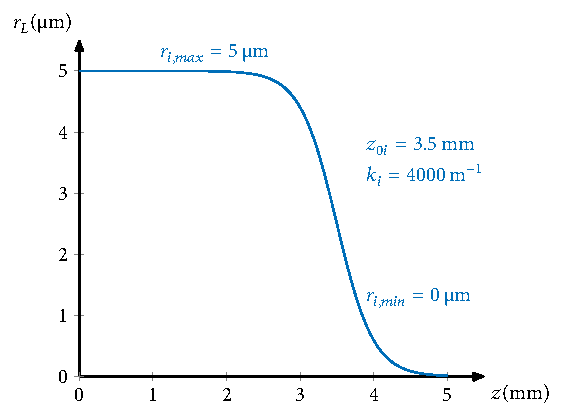
\includegraphics[width=\textwidth]{Figuras/ch4_ejsigm3.pdf}
    \caption{Primera sigmoide para la meseta}\label{fig:ch4_ssigma}
  \end{subcaptionblock}
  \begin{subcaptionblock}{.4\textwidth}
    \centering
    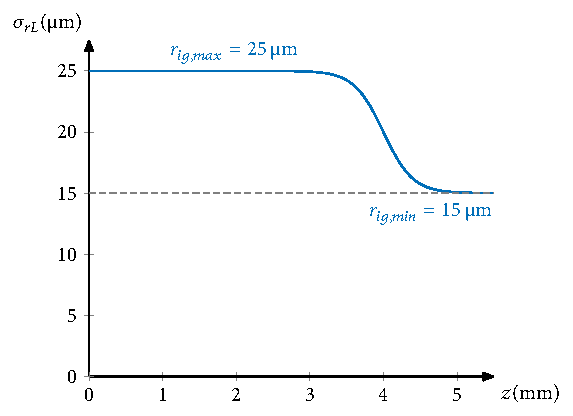
\includegraphics[width=\textwidth]{Figuras/ch4_ejsigm4.pdf}
    \caption{Segunda sigmoide para la falda}\label{fig:ch4_ssigmb}
  \end{subcaptionblock}
   \caption{Ejemplos de sigmoides para controlar completamente los perfiles. El eje de abscisas representa la longitud recorrida en milímetros $z$ (\unit{mm}) y el eje de ordenadas el radio de abundancia de \ce{Kr^{8+}} en micrómetros $r$ (\unit{\um})}
   \label{fig:4.19}
\end{figure}

\begin{longlisting}
  \caption{Fragmento del código Dagon dedicado a introducir la segunda sigmoide.}
  \inputminted[firstline=1, lastline=84]{fortran}{Programas/plasma3Dss.f90}
  \label{cod:4.5}
\end{longlisting}

\subsection{Variando el parámetro $r_{ig,max}$}\label{sec:4.2.1}
Este nuevo comienzo de las simulaciones empieza manteniendo $r_{ig,min}=\qty{15}{µm}$ y modificando el parámetro $r_{ig,max}$ entre \qty{15}{µm} y \qty{25}{µm} cada dos micrómetros. La finalidad es análoga a la buscada en la sección \ref{sec:4.1.1}, responder a la siguiente pregunta: ¿cuál es el efecto de modificar el radio de la frontera con \ce{Kr^{8+}} sobre la amplificación? En este caso, la segunda sigmoide o gaussiana representa la región que da hacia el exterior del canal, en lugar de hacia el interior, luego el radio escogido como constante es $r_{ig,min}$, en lugar de $r_{ig,max}$. En la Figura \ref{fig:4.20}, están representadas la pareja de sigmoides utilizadas.

\begin{figure}[htbp]
  \centering
  \begin{subcaptionblock}{.4\textwidth}
    \centering
    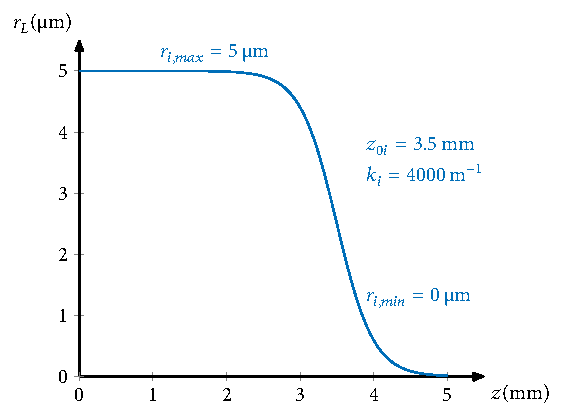
\includegraphics[width=\textwidth]{Figuras/ch4_ejsigm3.pdf}
    \caption{Primera sigmoide para la meseta}\label{fig:ch4_sigm1_rg}
  \end{subcaptionblock}
  \begin{subcaptionblock}{.4\textwidth}
    \centering
    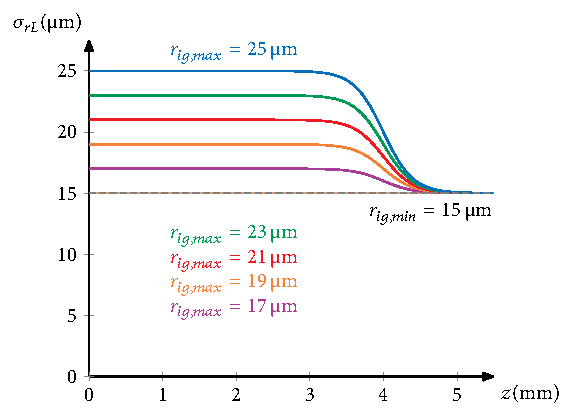
\includegraphics[width=\textwidth]{Figuras/ch4_sigm_rg.pdf}
    \caption{Segundas sigmoides para la falda}\label{fig:ch4_sigm2_rg}
  \end{subcaptionblock}
  \caption{Segunda sigmoide con $r_{ig,max}\in[\qty{15}{µm},\qty{25}{µm}]$, y $r_{ig,min}=\qty{15}{µm}$; manteniendo los valores de los parámetros $k_{ig}=\qty{5000}{m^{-1}}$ y $z_{0ig}=\qty{4}{mm}$.}
   \label{fig:4.20}
\end{figure}

Empezando por la situación sin la segunda sigmoide presente, con $r_{ig,min}=r_{ig,max}=\qty{15}{µm}$, la Figura \ref{fig:4.21} muestra la formación del valle de intensidad y una pequeña diferencia de profundidad en el perfil de fase. Como era de esperar, la anchura de la falda de la columna de plasma no puede reproducirse en este caso, puesto que para adaptar la parte inferior del perfil de intensidad es necesario tener un radio variable para la frontera exterior del canal, capaz de reflejar la variabilidad de la pendiente.

Por otro lado, cuando $r_{ig,min}=\qty{15}{µm}$ y $r_{ig,max}=\qty{17}{µm}$, ¡por primera vez el diámetro de la falda coincide con el experimento!, tal y como aparece en la Figura \ref{fig:4.22}. En esta ocasión, el radio máximo de la frontera exterior coincide aproximadamente con la coordenada radial donde se produce el cambio de pendiente de la curva de intensidad, adaptándose correctamente el ancho observable de la falda al perfil del laboratorio.

En las siguientes simulaciones (anexo \S\ref{anx:2}), aumentando $r_{ig,max}$ hasta alcanzar los \qty{25}{µm}, la anchura de los perfiles crece progresivamente, perdiendo completamente el acuerdo con el experimento. En cualquiera de los casos, la profundidad del perfil de fase mantiene una discrepancia importante, que podría solventarse recurriendo nuevamente a la distribución electrónica de la columna. 

\begin{figure}[htbp]
  \centering
  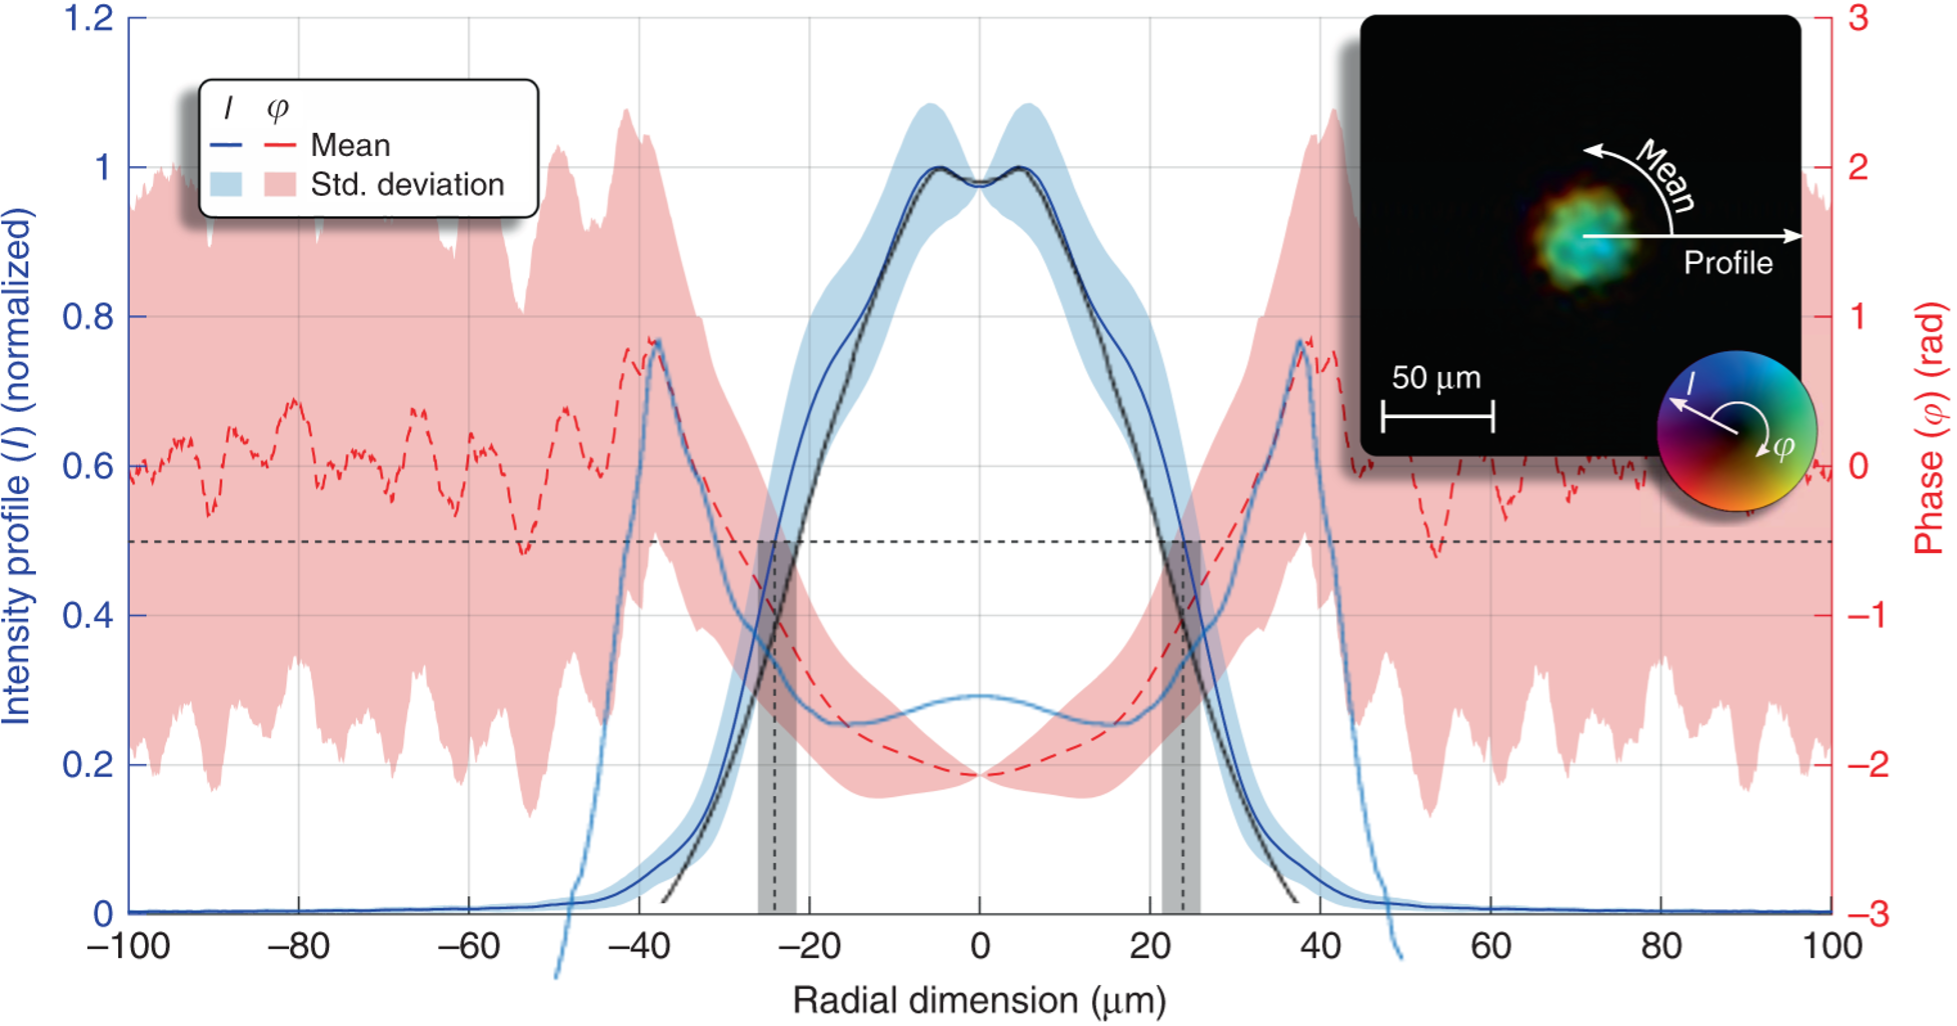
\includegraphics[width=0.7\textwidth]{Figuras/ch4_cmp41.png}
  \caption{Comparación entre los perfiles radiales de intensidad--fase con $r_{ig,min}=r_{ig,max}=\qty{15}{µm}$, manteniendo los valores de los parámetros $k_{ig}=\qty{5000}{m^{-1}}$ y $z_{0ig}=\qty{4}{mm}$; y el experimento.}
  \label{fig:4.21}
\end{figure}

\begin{figure}[htbp!]
  \centering
  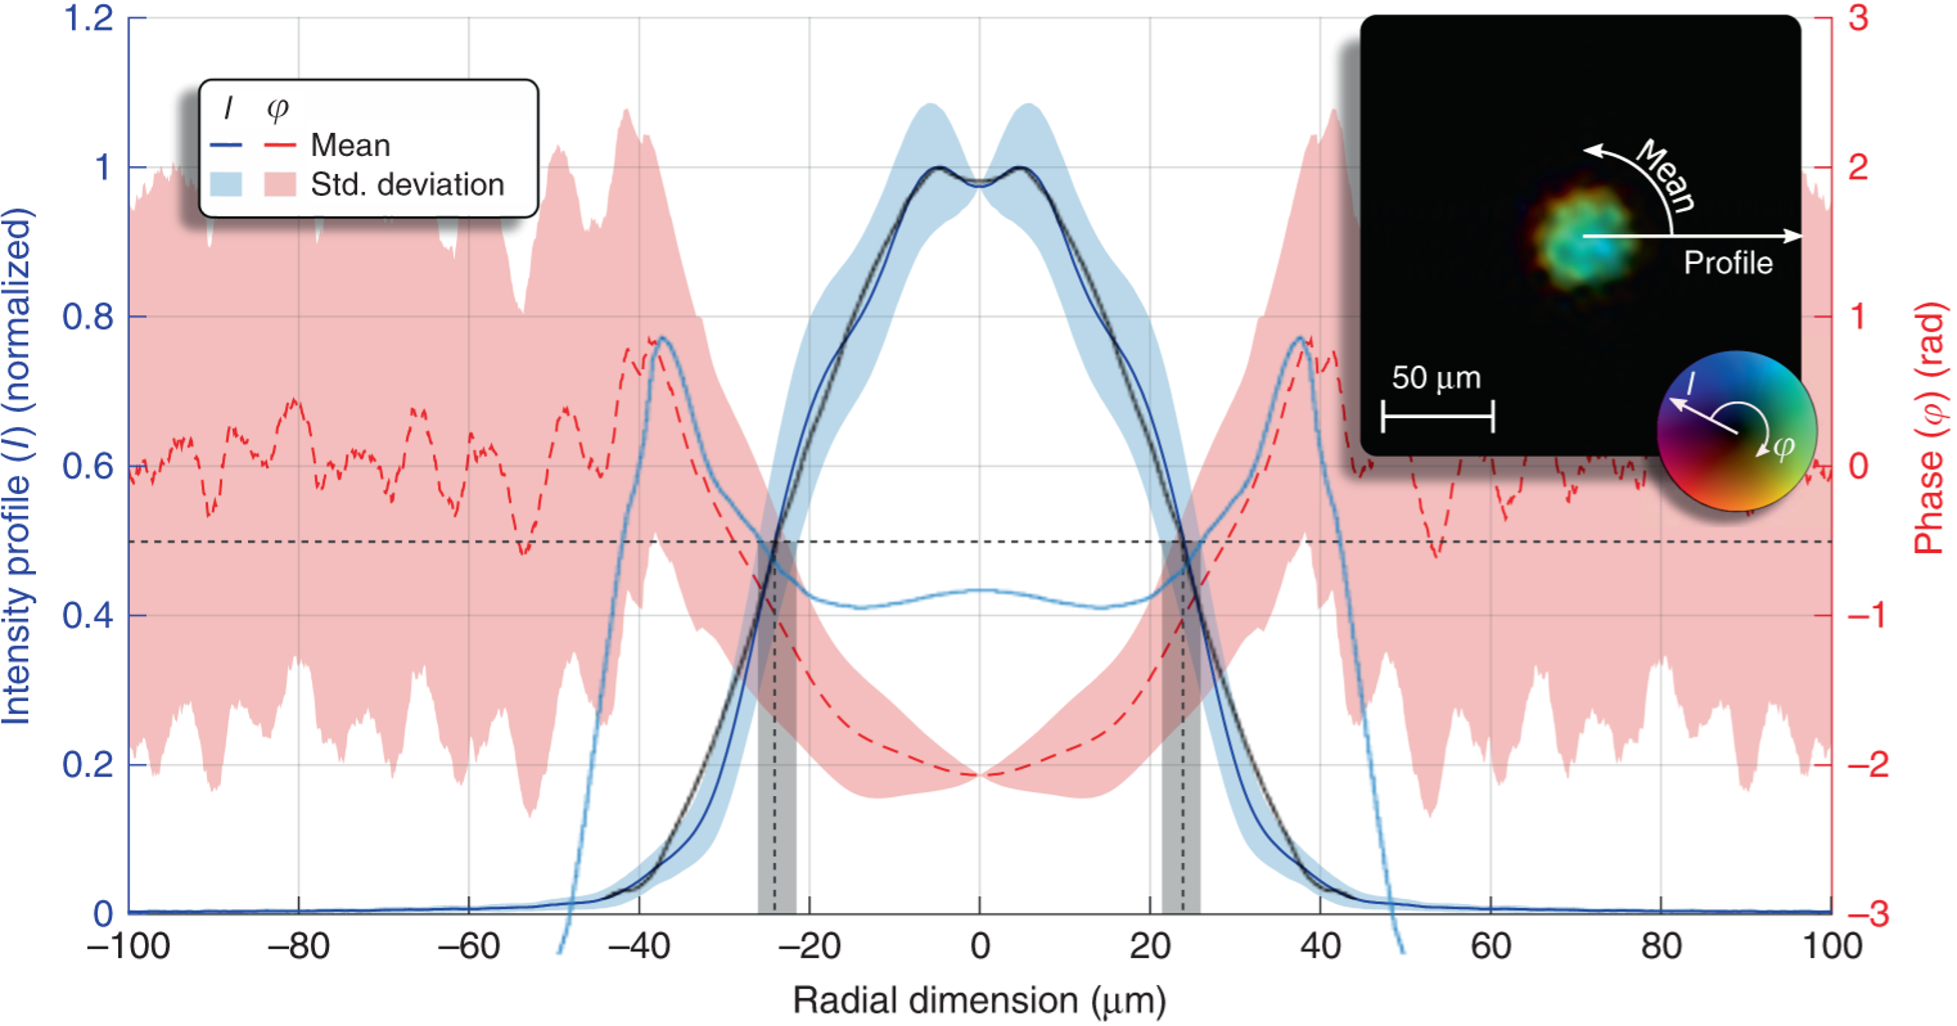
\includegraphics[width=0.7\textwidth]{Figuras/ch4_cmp42.png}
  \caption{Comparación entre los perfiles radiales de intensidad--fase con $r_{ig,min}=\qty{15}{µm}$ y $r_{ig,max}=\qty{17}{µm}$, manteniendo los valores de los parámetros $k_{ig}=\qty{5000}{m^{-1}}$ y $z_{0ig}=\qty{4}{mm}$; y el experimento.}
  \label{fig:4.22}
\end{figure}

La Tabla \ref{tab:4.6} muestra los parámetros utilizados para implementar la curva logística completa. De este modo, el parámetro $\sigma_{r}=\qty{15}{µm}$ es sustituido por los parámetros de la segunda sigmoide introducidos en el término cociente de exponenciales. Las mitades izquierda y derecha de las columnas recogen los parámetros de la primera sigmoide (meseta y valle de intensidad) y la segunda sigmoide (falda de intensidad), respectivamente.

\begin{table}[htpb]
  \centering
  \tiny
  \caption{Parámetros utilizados en las simulaciones con dos sigmoides, variando $r_{ig,max}$ (en azul) entre \qty{15}{µm} y \qty{25}{µm}. El símbolo del \enquote{tick} señala las simulaciones con buen acuerdo.}
  \label{tab:4.6}
  \begin{tabular}{>{\color{miazul}}SSSSSSSSSSSSSS}
  \toprule
  \multicolumn{4}{c}{Meseta | Falda} & & & & & & \\ 
  \cmidrule{1-4}\cmidrule(l){5-10}
  {$r_{i,max}$ | $r_{ig,max}$ (\unit{\um})} & {$r_{i,min}$ | $r_{ig,min}$ (\unit{\um})} & {$k_{i}$ | $k_{ig}$ (\unit{\mm^{-1}})} & {$z_{0i}$ | $z_{0ig}$ (\unit{mm})} & {\texttt{zshift}} & {\texttt{cen\_fac}} & {$\sigma_{z0}$ (\unit{mm})} & {$\sigma_{r0}$ (\unit{\um})} & {$z_{ion,1}$ (\unit{mm})} & {$z_{ion,2}$ (\unit{mm})} \\ 
  \midrule
  \numlist{5;15}  & \numlist{0;15}  & \numlist{4;5} & \numlist{3.5;4} & 0.75  & 0.3  & 2  & 15  & 0  & 3.75  \\
  \numlist{5;17} \checkmark  & \numlist{0;15}  & \numlist{4;5} & \numlist{3.5;4} & 0.75  & 0.3  & 2  & 15  & 0  & 3.75  \\
  \numlist{5;19}  & \numlist{0;15}  & \numlist{4;5} & \numlist{3.5;4} & 0.75  & 0.3  & 2  & 15  & 0  & 3.75  \\
  \numlist{5;21}  & \numlist{0;15}  & \numlist{4;5} & \numlist{3.5;4} & 0.75  & 0.3  & 2  & 15  & 0  & 3.75  \\
  \numlist{5;23}  & \numlist{0;15}  & \numlist{4;5} & \numlist{3.5;4} & 0.75  & 0.3  & 2  & 15  & 0  & 3.75  \\
  \numlist{5;25}  & \numlist{0;15}  & \numlist{4;5} & \numlist{3.5;4} & 0.75  & 0.3  & 2  & 15  & 0  & 3.75  \\ 
  \bottomrule
  \end{tabular}
\end{table}

\subsection{Variando el parámetro $z_{0ig}$}\label{sec:4.2.2}
Siguiendo el paralelismo establecido entre la sección \S\ref{sec:4.1} y esta sección \S\ref{sec:4.2}, y después de realizar las modificaciones del radio máximo en la frontera exterior del canal, es sencillo ejecutar las simulaciones análogas a las estudiadas durante la sección \ref{sec:4.1.2}. Volviendo a esta secuencia anterior, la misión es estudiar la influencia de la posición intermedia de la segunda sigmoide, alternando simultáneamente entre $r_{ig,max}=\qty{15}{µm}$ y $r_{ig,min}=\qty{25}{µm}$, como aparece en la Figura \ref{fig:4.23}.

Ahora, cuando la segunda sigmoide no existe, vuelve a suceder lo mismo que en la sección \S\ref{sec:4.2.1}. El valle central está formado, y la diferencia de profundidades del perfil de fase es pequeña, pero el ancho de la falda de intensidad necesita adaptarse al perfil experimental. Sin embargo, cuando $z_{0ig}=\qty{2}{mm}$, $r_{ig,max}=\qty{25}{µm}$ y $r_{ig,min}=\qty{15}{µm}$, se recupera el acuerdo entre simulación y experimento, excepto la región cóncava de la fase que permanece formándose. La Figura \ref{fig:4.24} presenta este segundo caso, 

Incrementando la coordenada del punto medio donde la curva logística toma su valor medio, el ajuste obtenido en el perfil de intensidad desaparece otra vez ---como muestra la Figura \ref{fig:4.25}---, debido a un aumento de la anchura de la falda y la aparición de sobreoscilaciones en la parte más baja. Este desplazamiento de la transición entre los radios máximo $r_{ig,max}$ y mínimo $r_{ig,min}$ hacia mayores longitudes axiales termina rompiendo la semejanza entre simulación y experimento. 

\begin{figure}[htbp]
  \centering
  \begin{subcaptionblock}{.4\textwidth}
    \centering
    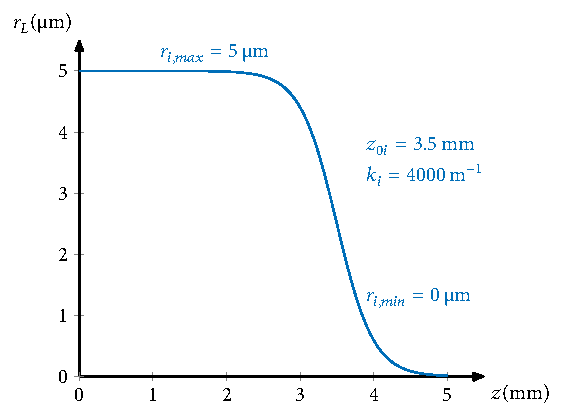
\includegraphics[width=\textwidth]{Figuras/ch4_ejsigm3.pdf}
    \caption{Primera sigmoide para la meseta}\label{fig:ch4_sigm1_rg}
  \end{subcaptionblock}
  \begin{subcaptionblock}{.4\textwidth}
    \centering
    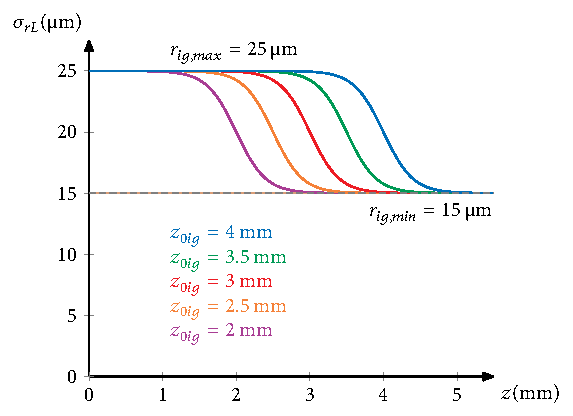
\includegraphics[width=\textwidth]{Figuras/ch4_sigm_z0g.pdf}
    \caption{Segundas sigmoides para la falda}\label{fig:ch4_sigm2_rg}
  \end{subcaptionblock}
  \caption{Segunda sigmoide con $z_{0ig}\in[\qty{2}{mm},\qty{4}{mm}]$ y $r_{ig,max}$ tomando valores alternativos entre \qty{15}{µm} y \qty{25}{µm}; manteniendo los valores de los parámetros $k_{ig}=\qty{5000}{m^{-1}}$ y $r_{ig,min}=\qty{15}{µm}$.}
   \label{fig:4.23}
\end{figure}

El fenómeno de las sobreoscilaciones producido a partir de $z_{0ig}=\qty{3}{mm}$ es debido a, probablemente, un aumento excesivo de la desviación estándar ---la magnitud de la sigmoide--- por encima de un cierto umbral. Reunidos en la Tabla \ref{tab:4.7} están todos los parámetros modificados de la curva logística durante su movimiento hacia mayores longitudes de propagación en la columna de plasma.

\begin{table}[htpb]
  \centering
  \tiny
  \caption{Parámetros utilizados en las simulaciones con dos sigmoides, variando $z_{0ig}$ (en azul) entre \qty{2}{mm} y \qty{4}{mm}. El símbolo del \enquote{tick} señala las simulaciones con buen acuerdo.}
  \label{tab:4.7}
  \begin{tabular}{>{\color{miazul}}SSS>{\color{miazul}}SSSSSSSSSSS}
  \toprule
  \multicolumn{4}{c}{Meseta | Falda} & & & & & & \\ 
  \cmidrule{1-4}\cmidrule(l){5-10}
  {$r_{i,max}$ | $r_{ig,max}$ (\unit{\um})} & {$r_{i,min}$ | $r_{ig,min}$ (\unit{\um})} & {$k_{i}$ | $k_{ig}$ (\unit{\mm^{-1}})} & {$z_{0i}$ | $z_{0ig}$ (\unit{mm})} & {\texttt{zshift}} & {\texttt{cen\_fac}} & {$\sigma_{z0}$ (\unit{mm})} & {$\sigma_{r0}$ (\unit{\um})} & {$z_{ion,1}$ (\unit{mm})} & {$z_{ion,2}$ (\unit{mm})} \\ 
  \midrule
  \numlist{5;15}  & \numlist{0;15}  & \numlist{4;5} & \numlist{3.5;2} & 0.75  & 0.3  & 2  & 15  & 0  & 3.75  \\
  \numlist{5;25} \checkmark  & \numlist{0;15}  & \numlist{4;5} & \numlist{3.5;2} & 0.75  & 0.3  & 2  & 15  & 0  & 3.75  \\
  \numlist{5;15}  & \numlist{0;15}  & \numlist{4;5} & \numlist{3.5;2.5} & 0.75  & 0.3  & 2  & 15  & 0  & 3.75  \\
  \numlist{5;25} \checkmark  & \numlist{0;15}  & \numlist{4;5} & \numlist{3.5;2.5} & 0.75  & 0.3  & 2  & 15  & 0  & 3.75  \\
  \numlist{5;15}  & \numlist{0;15}  & \numlist{4;5} & \numlist{3.5;3} & 0.75  & 0.3  & 2  & 15  & 0  & 3.75  \\
  \numlist{5;25}  & \numlist{0;15}  & \numlist{4;5} & \numlist{3.5;3} & 0.75  & 0.3  & 2  & 15  & 0  & 3.75  \\ 
  \numlist{5;15}  & \numlist{0;15}  & \numlist{4;5} & \numlist{3.5;3.5} & 0.75  & 0.3  & 2  & 15  & 0  & 3.75  \\
  \numlist{5;25}  & \numlist{0;15}  & \numlist{4;5} & \numlist{3.5;3.5} & 0.75  & 0.3  & 2  & 15  & 0  & 3.75  \\ 
  \numlist{5;15}  & \numlist{0;15}  & \numlist{4;5} & \numlist{3.5;4} & 0.75  & 0.3  & 2  & 15  & 0  & 3.75  \\
  \numlist{5;25}  & \numlist{0;15}  & \numlist{4;5} & \numlist{3.5;4} & 0.75  & 0.3  & 2  & 15  & 0  & 3.75  \\ 
  \bottomrule
  \end{tabular}
\end{table}

\begin{figure}[htbp!]
  \centering
  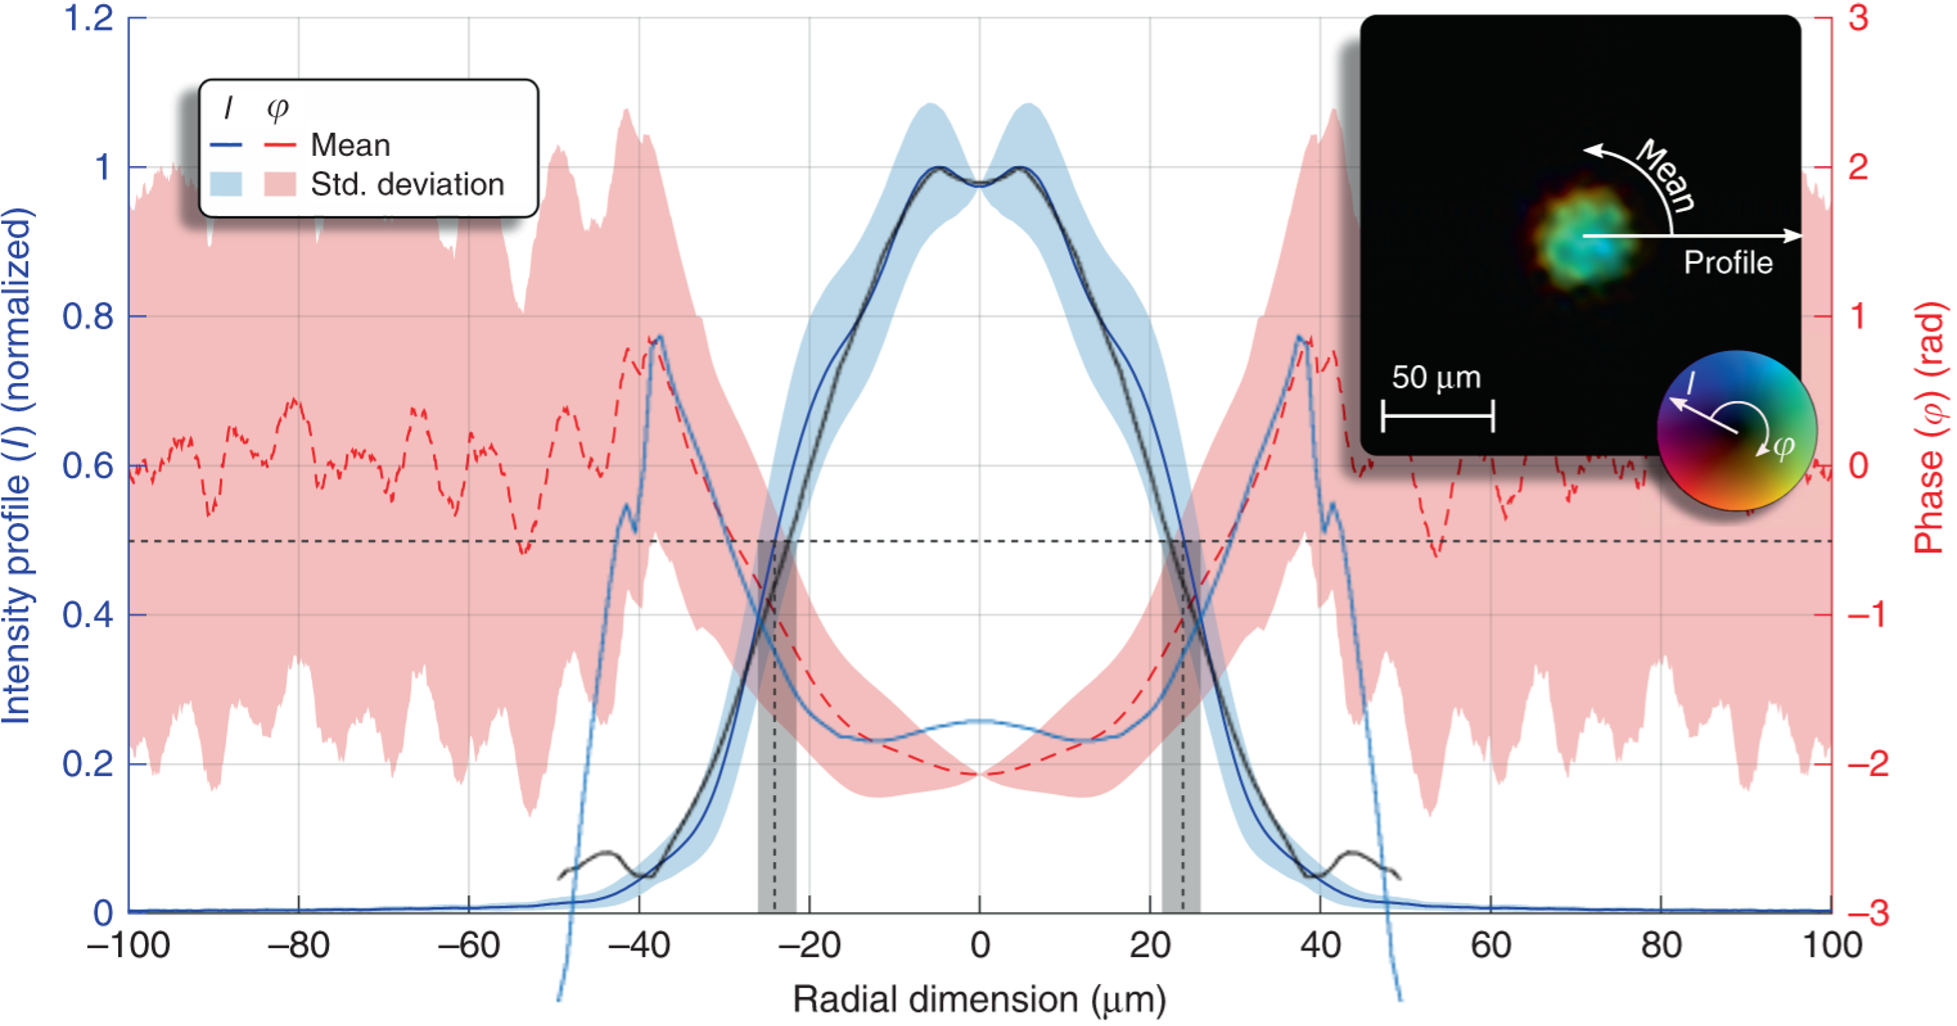
\includegraphics[width=0.75\textwidth]{Figuras/ch4_cmp51.png}
  \caption{Comparación entre los perfiles radiales de intensidad--fase con $r_{ig,min}=\qty{15}{µm}$ y $r_{ig,max}=\qty{25}{µm}$, manteniendo los valores de los parámetros $k_{ig}=\qty{5000}{m^{-1}}$ y $z_{0ig}=\qty{2}{mm}$; y el experimento.}
  \label{fig:4.24}
\end{figure}

\begin{figure}[htbp!]
  \centering
  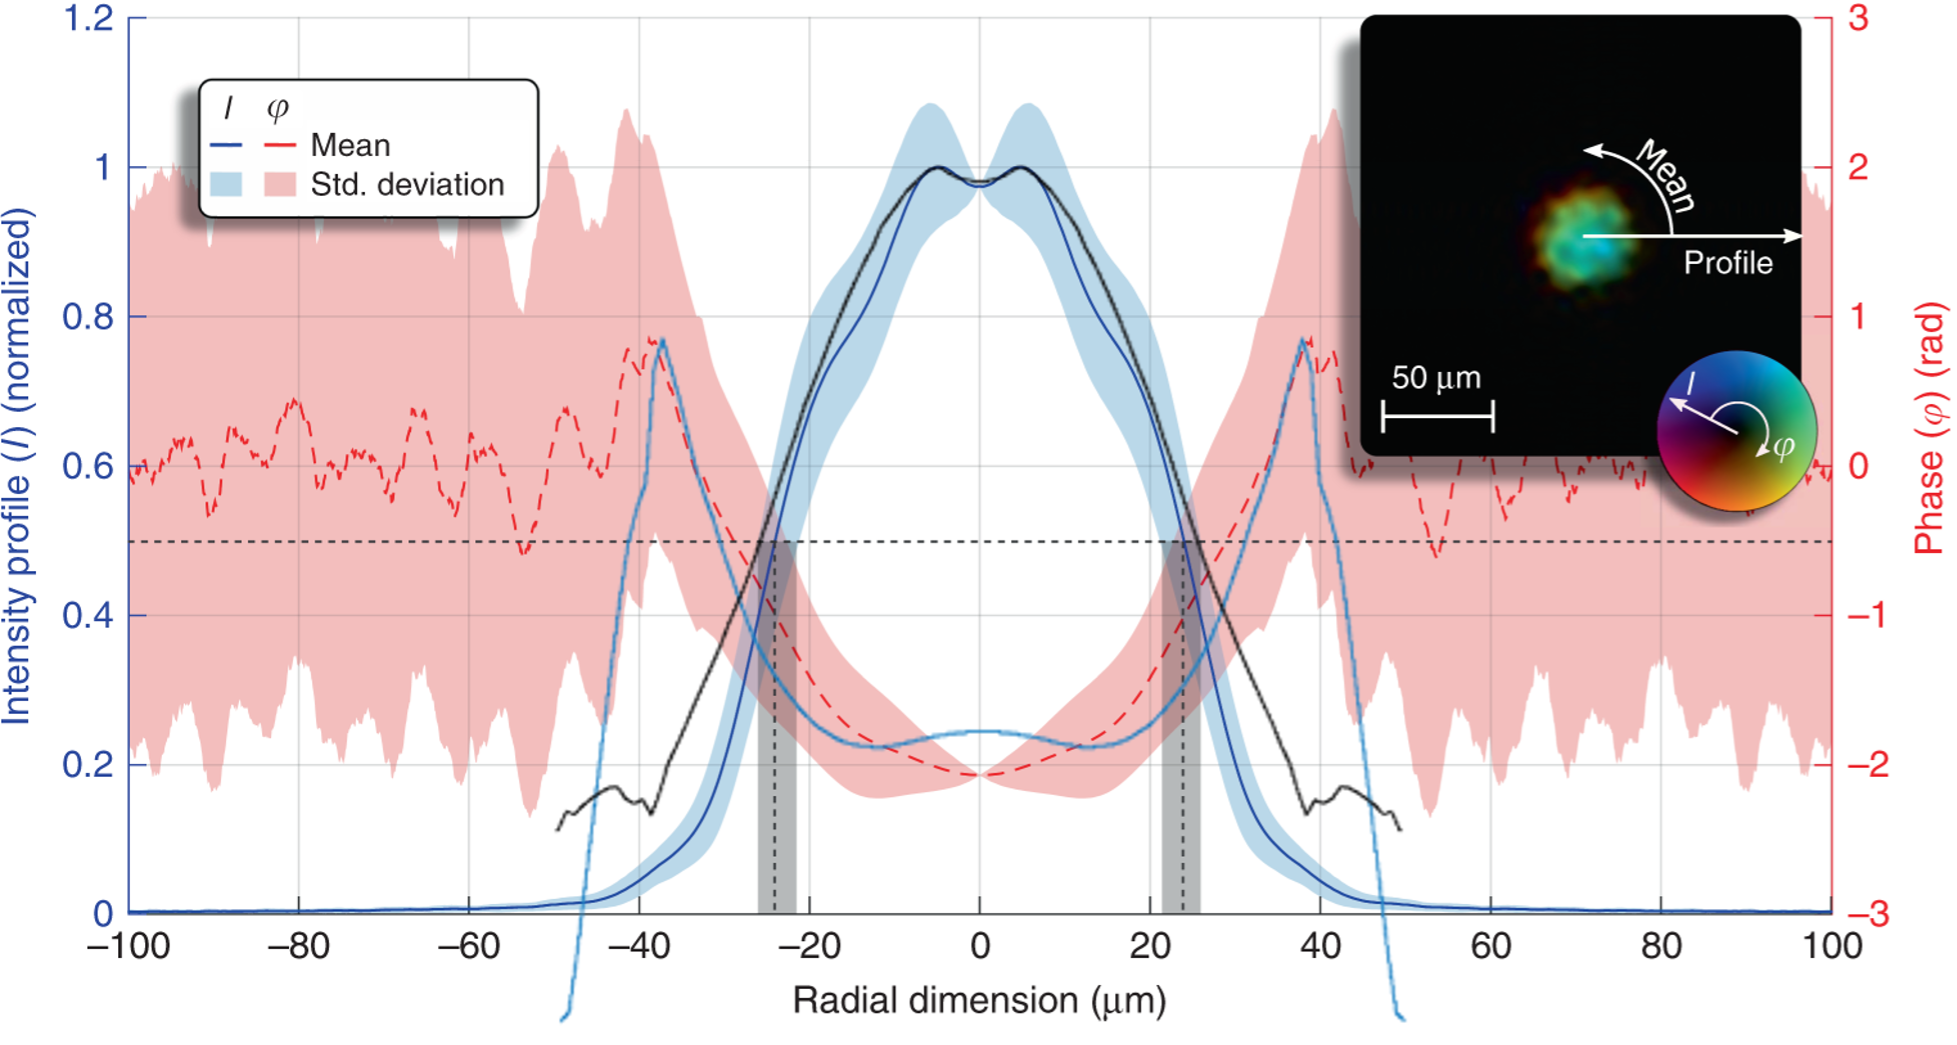
\includegraphics[width=0.75\textwidth]{Figuras/ch4_cmp52.png}
  \caption{Comparación entre los perfiles radiales de intensidad--fase con $r_{ig,min}=\qty{15}{µm}$ y $r_{ig,max}=\qty{25}{µm}$, manteniendo los valores de los parámetros $k_{ig}=\qty{5000}{m^{-1}}$ y $z_{0ig}=\qty{3}{mm}$; y el experimento.}
  \label{fig:4.25}
\end{figure}

\subsection{Variando el parámetro $k_{ig}$}\label{4.2.3}
Finalmente, apoyándose en las observaciones realizadas en la anterior sección \S\ref{sec:4.2.2}, el último grupo de simulaciones está destinado a conocer los efectos de la rapidez de la transición entre los radios mínimo $r_{ig,min}=\qty{15}{µm}$ y máximo $r_{ig,max}=\qty{25}{µm}$, centrándose en la región exterior del perfil a través del parámetro $k_{0ig}$. La Figura \ref{fig:4.26} recoge el último conjunto de parejas de sigmoides empleadas.

Los resultados obtenidos demuestran un comportamiento muy parecido, originándose un perfil de intensidad con una anchura excesivamente elevada, capaz de englobar completamente la curva experimental. En representación de este comportamiento, se escoge la Figura \ref{fig:4.27}, dejando las demás para consultar si es necesario en el anexo \S\ref{anx:2}. Aunque el incremento de la tasa de cambio termina distorsionando el resultado, escogiendo una coordenada media $z_{0ig}<\qty{4}{µm}$ podría haberse reducido el ancho de la falda, para intentar ajustarla correctamente.

\begin{figure}[htbp]
  \centering
  \begin{subcaptionblock}{.4\textwidth}
    \centering
    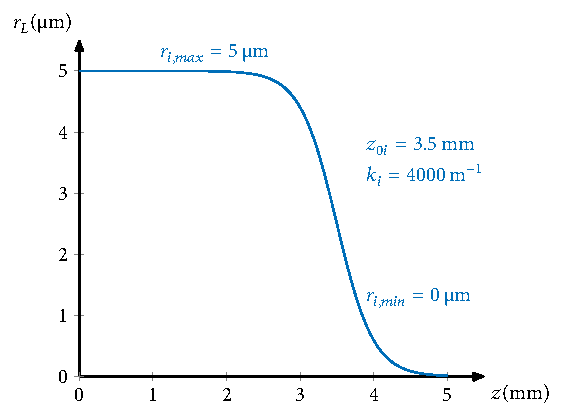
\includegraphics[width=\textwidth]{Figuras/ch4_ejsigm3.pdf}
    \caption{Primera sigmoide para la meseta}\label{fig:ch4_sigm1_rg}
  \end{subcaptionblock}
  \begin{subcaptionblock}{.4\textwidth}
    \centering
    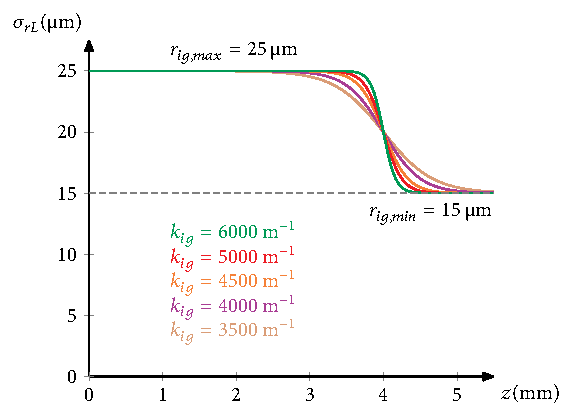
\includegraphics[width=\textwidth]{Figuras/ch4_sigm_kg.pdf}
    \caption{Segundas sigmoides para la falda}\label{fig:ch4_sigm2_rg}
  \end{subcaptionblock}
  \caption{Segunda sigmoide con el parámetro $k_{ig}\in[\qty{3500}{m^{-1}},\qty{6000}{m^{-1}}]$; manteniendo los valores de los parámetros $r_{ig,max}=\qty{25}{µm}$, $r_{ig,min}=\qty{15}{µm}$ y $z_{0ig}=\qty{4}{mm}$.}
   \label{fig:4.26}
\end{figure}

Terminada esta sección \S\ref{sec:4.2}, pueden extraerse las conclusiones a cerca de los resultados. La combinación de dos sigmoides para el modelado completo del perfil de intensidad es bueno, pero no alcanza a ser completamente satisfactorio. La anchura de la falda puede conseguirse fácilmente mediante esta segunda curva logística, pero el cambio de pendiente de la falda no aparece mediante este recurso. 

\begin{figure}[htbp]
  \centering
  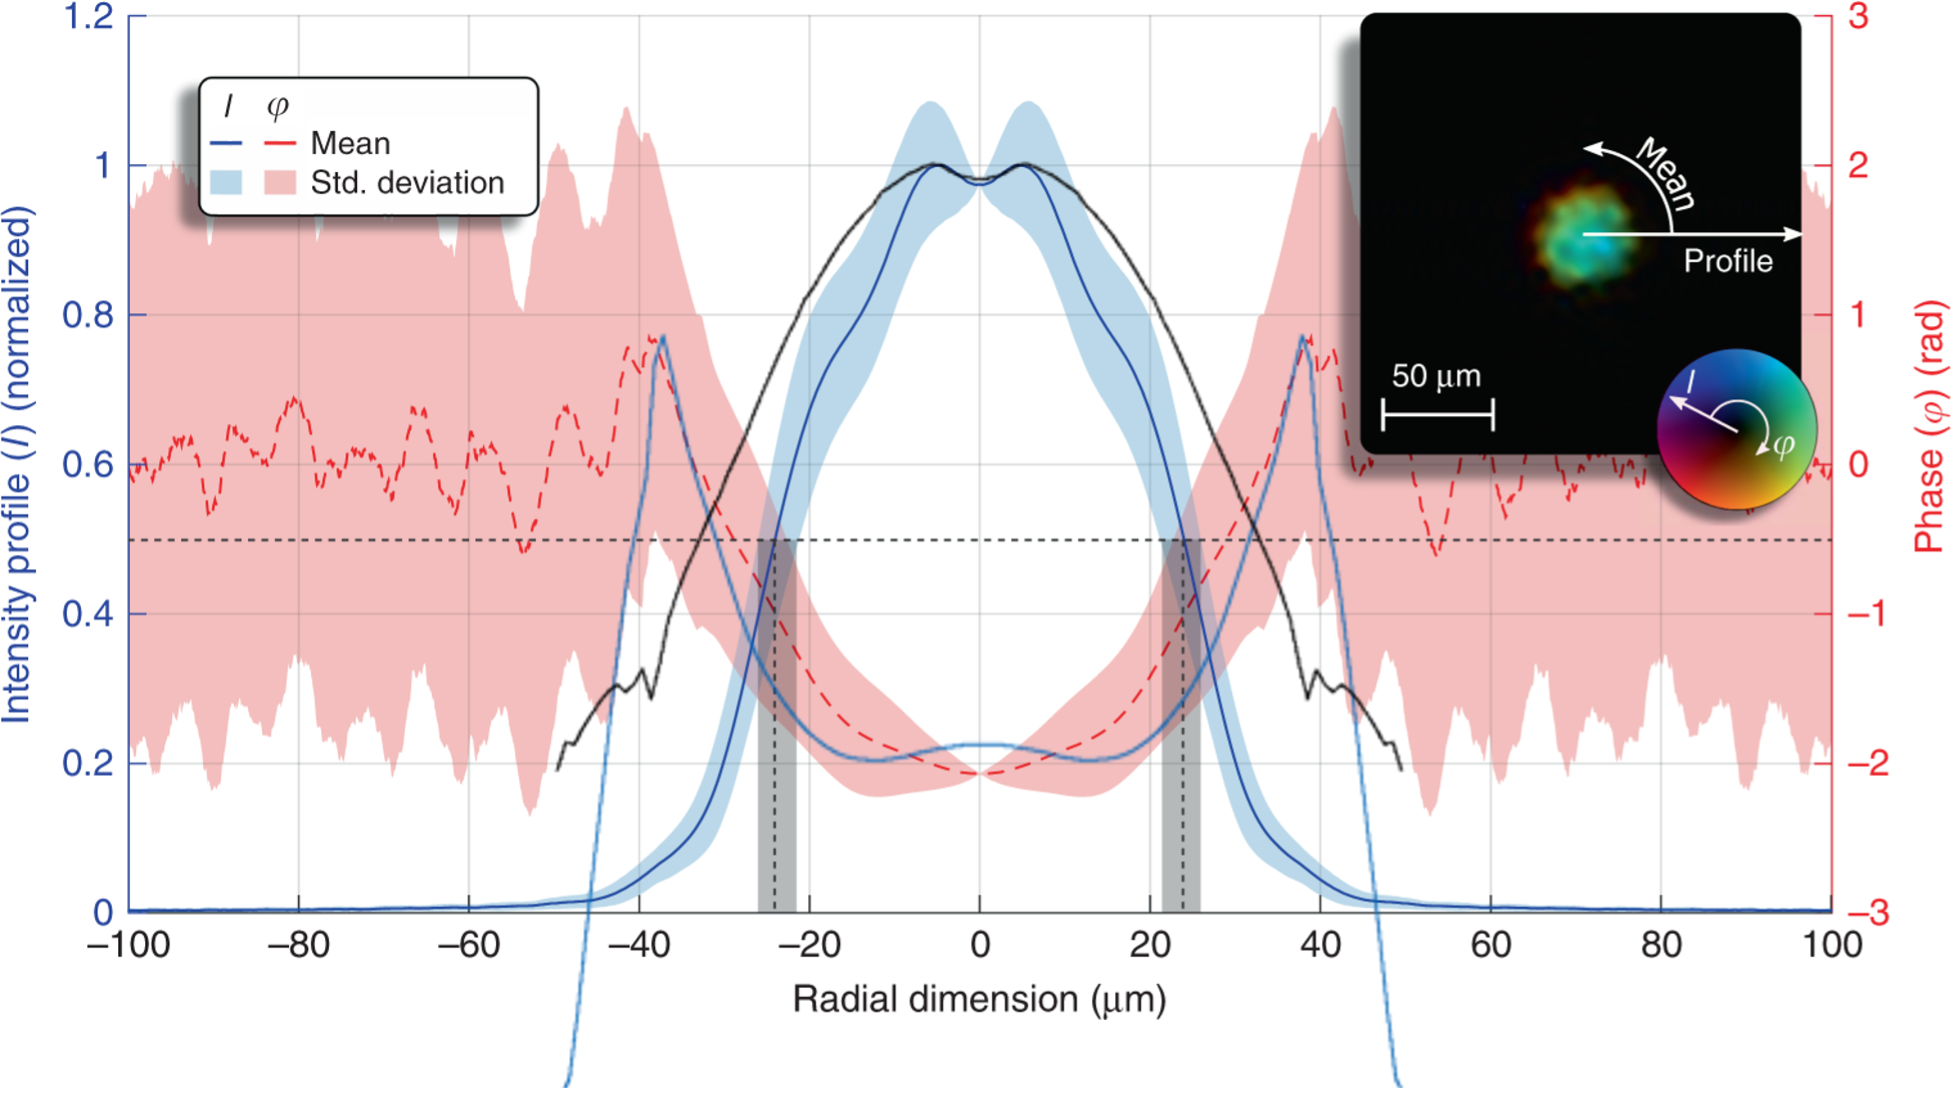
\includegraphics[width=0.75\textwidth]{Figuras/ch4_cmp61.png}
  \caption{Comparación entre los perfiles radiales de intensidad--fase con $k_{ig}=\qty{4500}{m^{-1}}$, manteniendo los valores de los parámetros $r_{ig,min}=\qty{15}{µm}$, $r_{ig,max}=\qty{25}{µm}$ y $z_{0ig}=\qty{4}{mm}$; y el experimento.}
  \label{fig:4.27}
\end{figure}

En cierto modo, el perfil obtenido es un \enquote{promedio} entre la parte superior e inferior de la curva, capaz en algunos casos de aproximar los anchos de ambas partes. Sin embargo, para conseguir ajustar completamente la curva es necesario introducir un cambio en la pendiente, sujeto de análisis en la sección \S\ref{sec:4.3}. La Tabla \ref{tab:4.8} tiene recogidos los últimos parámetros introducidos. 

\begin{table}[htpb]
  \centering
  \tiny
  \caption{Parámetros utilizados en las simulaciones con dos sigmoides, variando $k_{ig}$ (en azul) entre \qty{3500}{m^{-1}} y \qty{6000}{m^{-1}}. El símbolo del \enquote{tick} señala las simulaciones con buen acuerdo.}
  \label{tab:4.8}
  \begin{tabular}{SS>{\color{miazul}}SSSSSSSSSSSS}
  \toprule
  \multicolumn{4}{c}{Meseta | Falda} & & & & & & \\ 
  \cmidrule{1-4}\cmidrule(l){5-10}
  {$r_{i,max}$ | $r_{ig,max}$ (\unit{\um})} & {$r_{i,min}$ | $r_{ig,min}$ (\unit{\um})} & {$k_{i}$ | $k_{ig}$ (\unit{\mm^{-1}})} & {$z_{0i}$ | $z_{0ig}$ (\unit{mm})} & {\texttt{zshift}} & {\texttt{cen\_fac}} & {$\sigma_{z0}$ (\unit{mm})} & {$\sigma_{r0}$ (\unit{\um})} & {$z_{ion,1}$ (\unit{mm})} & {$z_{ion,2}$ (\unit{mm})} \\ 
  \midrule
  \numlist{5;25}  & \numlist{0;15}  & \numlist{4;3.5} & \numlist{3.5;4} & 0.75  & 0.3  & 2  & 15  & 0  & 3.75  \\
  \numlist{5;25}  & \numlist{0;15}  & \numlist{4;4} & \numlist{3.5;4} & 0.75  & 0.3  & 2  & 15  & 0  & 3.75  \\
  \numlist{5;25}  & \numlist{0;15}  & \numlist{4;4.5} & \numlist{3.5;4} & 0.75  & 0.3  & 2  & 15  & 0  & 3.75  \\
  \numlist{5;25}  & \numlist{0;15}  & \numlist{4;5} & \numlist{3.5;4} & 0.75  & 0.3  & 2  & 15  & 0  & 3.75  \\ 
  \numlist{5;25}  & \numlist{0;15}  & \numlist{4;6} & \numlist{3.5;4} & 0.75  & 0.3  & 2  & 15  & 0  & 3.75  \\ 
  \bottomrule
  \end{tabular}
\end{table}

\section{Ajuste de la densidad de iones con funciones exponenciales}\label{sec:4.3}
Asumiendo las limitaciones de emplear la combinación de funciones sigmoides para controlar la curva, esta sección \S\ref{sec:4.3} elimina ambas curvas logísticas, introducidas a lo largo de la columna de plasma. En su lugar, el objetivo consiste en reemplazarlas por una sola función exponencial que juegue el papel del término cociente de exponenciales en la ecuación \eqref{eq:3.19a}, donde estaban introducidas las sigmoides.

De esta manera, esta función tiene que ajustar el ancho del perfil de intensidad totalmente, adaptándose por tanto al cambio de pendiente regular que se produce aproximadamente cuando $r=\qty{17}{µm}$, separando el  valle de intensidad y la falda de la distribución radial. Partiendo de la influencia de los parámetros estudiados, una sugerencia de función interesante a utilizar es una exponencial dividida en dos tramos. Un primer tramo horizontal hasta un radio del canal $r_{u}$ próximo a la variación de la pendiente, y un segundo tramo exponencial para radios mayores.

En resumen, la función tiene un parámetro auxiliar $r_{u}$ que fragmenta la curva de intensidad en dos partes, una para radios $r<r_{u}$ y otra para radios $r\geq r_{u}$, donde la pendiente tiene que cambiar de forma continua. La condición de continuidad es fundamental para mantener el buen comportamiento del perfil radial, aunque no es necesaria la derivabilidad de la función exponencial para implementarla en Dagon. La función exponencial a trozos introducida es 
\begin{equation}\label{eq:4.1}
  f(r) =  
  \begin{cases}
    \frac{\exp\left(-\frac{\max(r,r_{L})^{2}}{2 \sigma_{L}^{2}}\right)}{\exp\left(-\frac{r_{L}^{2}}{2 \sigma_{L}^{2}}\right)}, & \text{si $r<r_{u}$}, \\
    A\exp\left(-\frac{r^{2}}{\sigma_{u}^{2}}\right), & \text{si $r\geq r_{u}$},
  \end{cases}
\end{equation}
junto con la condición de continuidad 
\begin{equation}\label{eq:4.2}
  A = f(r_{u})\exp\bigg(\frac{r_{u}}{\sigma_{u}}\bigg)^{2}.
\end{equation}

Hay que mencionar que el coeficiente $A$ viene determinado adicionalmente por el hecho de que $r_{L}<r_{u}$, pues retoma el valor $r_{L}=\qty{5}{µm}$ anterior a la introducción de las sigmoides, y $r_{u}$ es la coordenada radial asociada a la variación de la pendiente de la falda, siempre mayor que este parámetro. Una vez establecida la función exponencial, es importante comprobar previamente su comportamiento antes de introducirla definitivamente en Dagon, escribiendo un nuevo programa en MATLAB. El código \ref{cod:4.6} muestra este programa de MATLAB completo.

\begin{listing}[htbp]
  \caption{Programa auxiliar de MATLAB para representar la función exponencial por tramos.} 
  \inputminted[firstline=1, lastline=27]{matlab}{Programas/f_trozos.m}
  \label{cod:4.6}
\end{listing}

En realidad, los parámetros introducidos también incluyen las desviaciones típicas de ambos radios $\sigma_{L}$ y $\sigma_{u}$, puesto que las exponenciales siguen manteniendo la forma de distribución gaussiana utilizada durante las anteriores secciones. Además, el código \ref{cod:4.6} es útil como primera aproximación para introducir los nuevos cambios dentro de la subrutina \texttt{fillplasma} en Dagon. Tras verificar la adecuación de la función a las expectativas previstas, el último paso es implementar los cambios en Dagon, escritos en el código \ref{cod:4.7}.

\begin{longlisting}
  \caption{Fragmento del código Dagon dedicado a introducir la función exponencial.}
  \inputminted[firstline=1, lastline=80]{fortran}{Programas/plasma3Dt.f90}
  \label{cod:4.7}
\end{longlisting}

Señalar que el parámetro  $\texttt{cen\_fac}=0.075$ también ha sido modificado, en lugar del valor  $\texttt{cen\_fac}=0.03$ fijado en todas las simulaciones previas. Esta disminución de la densidad electrónica en la segunda región sobreionizada, responde a la necesidad de comparar los resultados obtenidos con proyectos realizados anteriormente donde también fueron estudiados estos aspectos relativos a la amplificación \acrshort{xuv}.

Las siguientes secciones presentan la variación de los dos parámetros fundamentales de la función exponencial, el radio $r_{u}$ y la desviación estándar $\sigma_{u}$. A continuación se realiza la introducción del \acrshort{oam} en la semilla, terminando con algunos comentarios a cerca del papel de la amplificación del ruido en los perfiles de intensidad-fase.

\subsection{Variando el parámetro $r_{u}$}\label{sec:4.3.1}
El radio a partir del cuál la función exponencial diseñada cambia de un tramo al siguiente es fundamental para conseguir el cambio de pendiente deseado. En primer lugar, la parte para $r<r_{u}$ está encargada de formar adecuadamente el valle de intensidad, mientras que, en segundo lugar, la parte para $r\geq r_{u}$ tiene que originar la variación de la pendiente. Globalmente, la anchura tiene que ajustarse correctamente en toda la curva, y el perfil de fase tener la profundidad adecuada.

Para responder a la siguiente pregunta: ¿cómo influye la posición de la transición de ambos tramos exponenciales a la anchura de la falda de intensidad?, es razonable hacer variar el parámetro $r_{u}$ entre \qty{10}{µm} y \qty{20}{µm}, abarcando la coordenada $z \sim \qty{17}{µm}$ donde sucede el cambio de pendiente. Los demás parámetros se mantienen constantes, y pueden consultarse en la Tabla \ref{tab:4.9}. A modo de ejemplo, la Figura \ref{fig:4.28} representa la función exponencial utilizada, cuando $r_{u}=\qty{10}{µm}$. 

\begin{figure}[htbp]
  \centering
  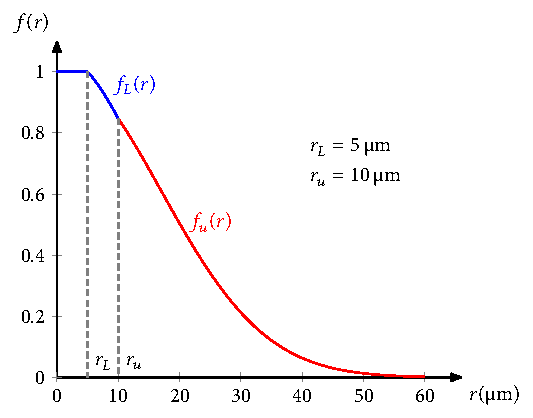
\includegraphics[width=0.45\textwidth]{Figuras/ch4_fexp1.pdf}
  \caption{Función exponencial con $r_{u}=\qty{10}{µm}$, manteniendo los valores de los parámetros $r_{L}=\qty{5}{µm}$, $\sigma_{L}=\qty{15}{µm}$ y $\sigma_{u}=\qty{17}{mm}$.}
  \label{fig:4.28}
\end{figure}

Observando detenidamente los perfiles radiales de intensidad y fase extraídos en este caso, mostrados en las Figuras \ref{fig:ch4_int71} y \ref{fig:ch4_fs71}, ¡puede apreciarse un ligero cambio en la tendencia de la falda en $r=\qty{10}{µm}$! La variación es muy liviana, pero establece un precedente nunca antes alcanzado.

\begin{figure}[htbp]
  \centering
  \begin{subcaptionblock}{.4\textwidth}
    \centering
    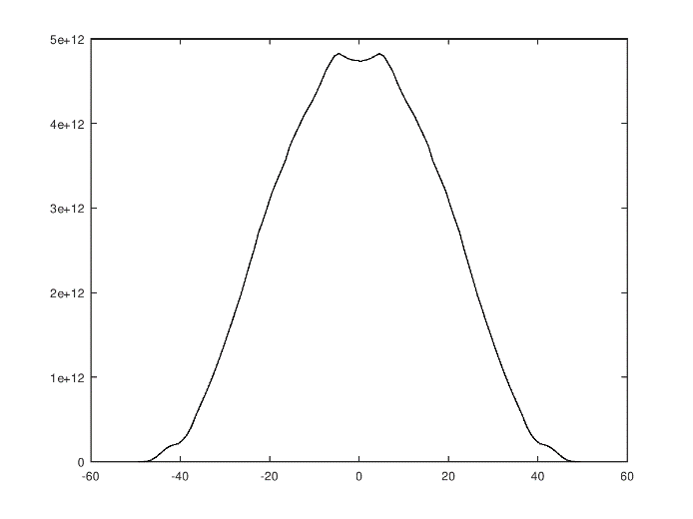
\includegraphics[width=\textwidth]{Figuras/ch4_int71.png}
    \caption{Perfil radial de intensidad (\unit{W/cm^2}) frente al radio (\unit{µm})}\label{fig:ch4_int71}
  \end{subcaptionblock}
  \begin{subcaptionblock}{.4\textwidth}
    \centering
    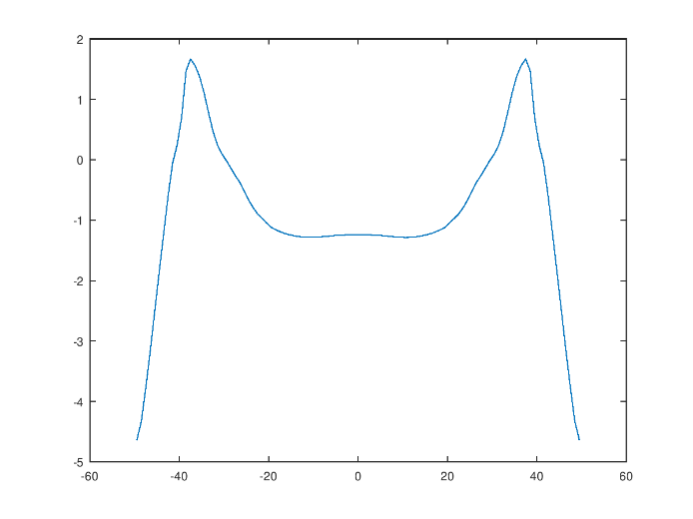
\includegraphics[width=\textwidth]{Figuras/ch4_fs71.png}
    \caption{Perfil radial de fase (\unit{rad}) frente al radio (\unit{µm})}\label{fig:ch4_fs71}
  \end{subcaptionblock}
   \caption{Distribución radial de intensidad--fase con $r_{u}=\qty{10}{µm}$, manteniendo los valores de los parámetros $r_{L}=\qty{5}{µm}$, $\sigma_{L}=\qty{15}{µm}$ y $\sigma_{u}=\qty{17}{µm}$.}
   \label{fig:4.29}
\end{figure}

\begin{figure}[htbp]
  \centering
  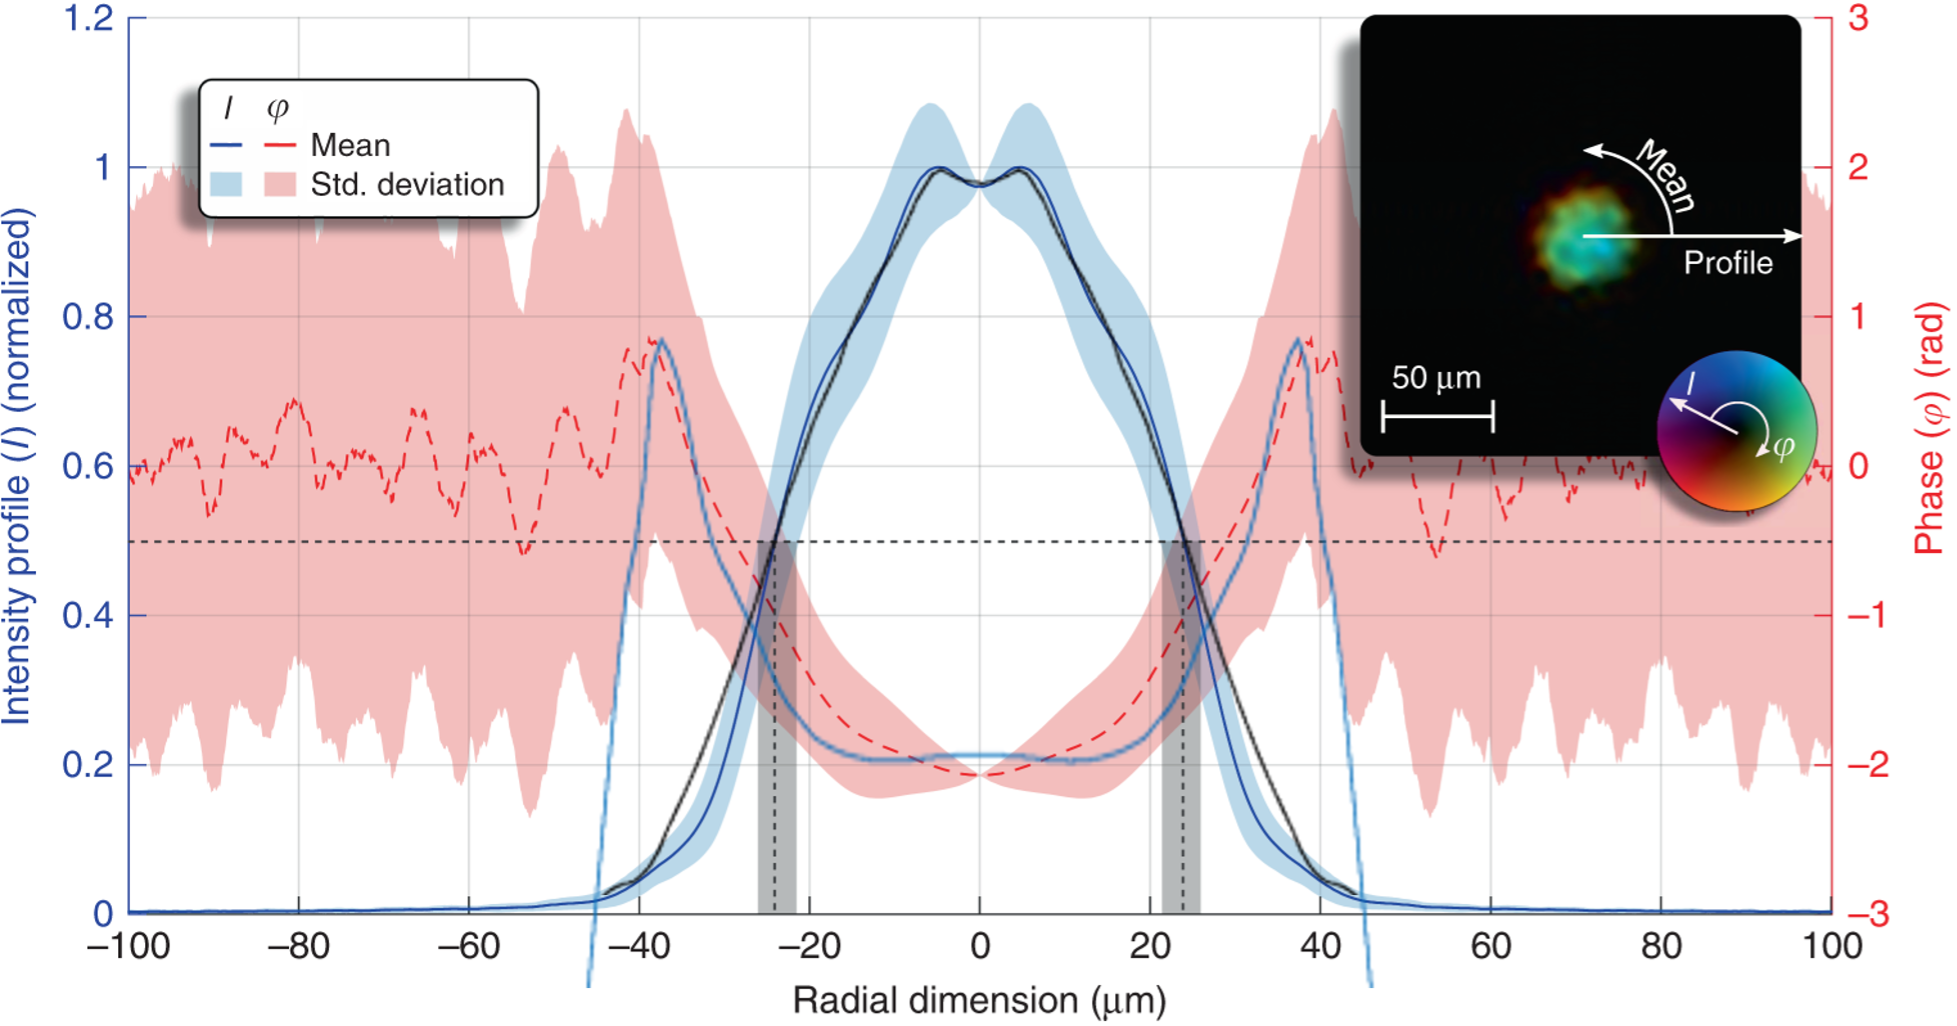
\includegraphics[width=0.75\textwidth]{Figuras/ch4_cmp71.png}
  \caption{Comparación entre los perfiles radiales de intensidad--fase con $r_{u}=\qty{10}{µm}$, manteniendo los valores de los parámetros $r_{L}=\qty{5}{µm}$, $\sigma_{L}=\qty{15}{µm}$ y $\sigma_{u}=\qty{17}{µm}$; y el experimento.}
  \label{fig:4.30}
\end{figure}

El solapamiento de la Figura \ref{fig:4.30} compara estos resultados, mostrando un ajuste muy bueno entre los perfiles de intensidad y fase. La sobreionización en la primera región del canal es capaz de originar el valle central de intensidad, y el pequeño cambio en la pendiente de la intensidad en la simulación coincide razonablemente bien con los resultados del experimento. Además, el perfil de fase también mantiene una profundidad entre valle y picos aceptable.

Por otro lado, en cuanto a los aspectos negativos, la parte inferior de la falda (a partir de $r=\qty{20}{µm}$) comienza a separarse de la curva base, mientras que concavidad del perfil de fase sigue formándose. Sin embargo, aumentando el radio de la exponencial por tramos hasta $r_{u}=\qty{15}{µm}$ ---plasmado en la Figura \ref{fig:4.31}---, el cambio de pendiente es desplazado hacia este radio superior, desacoplándose ambos perfiles de intensidad en la parte de la falda, como era de esperar.

Este comportamiento se reproduce en todas las simulaciones realizadas en este grupo, es decir, variando $r_{u}$ más allá de \qty{10}{µm}, los cambios de tendencia se difuminan progresivamente hasta desaparecer completamente en $r_{u}=\qty{20}{µm}$. Estas imágenes pueden consultarse en el anexo \S\ref{anx:3} para confirmar estas observaciones. La siguiente sección \S\ref{sec:4.3.2} emplea el mismo procedimiento, pero variando la desviación típica $\sigma_{u}$ de la exponencial.

\begin{figure}[htbp]
  \centering
  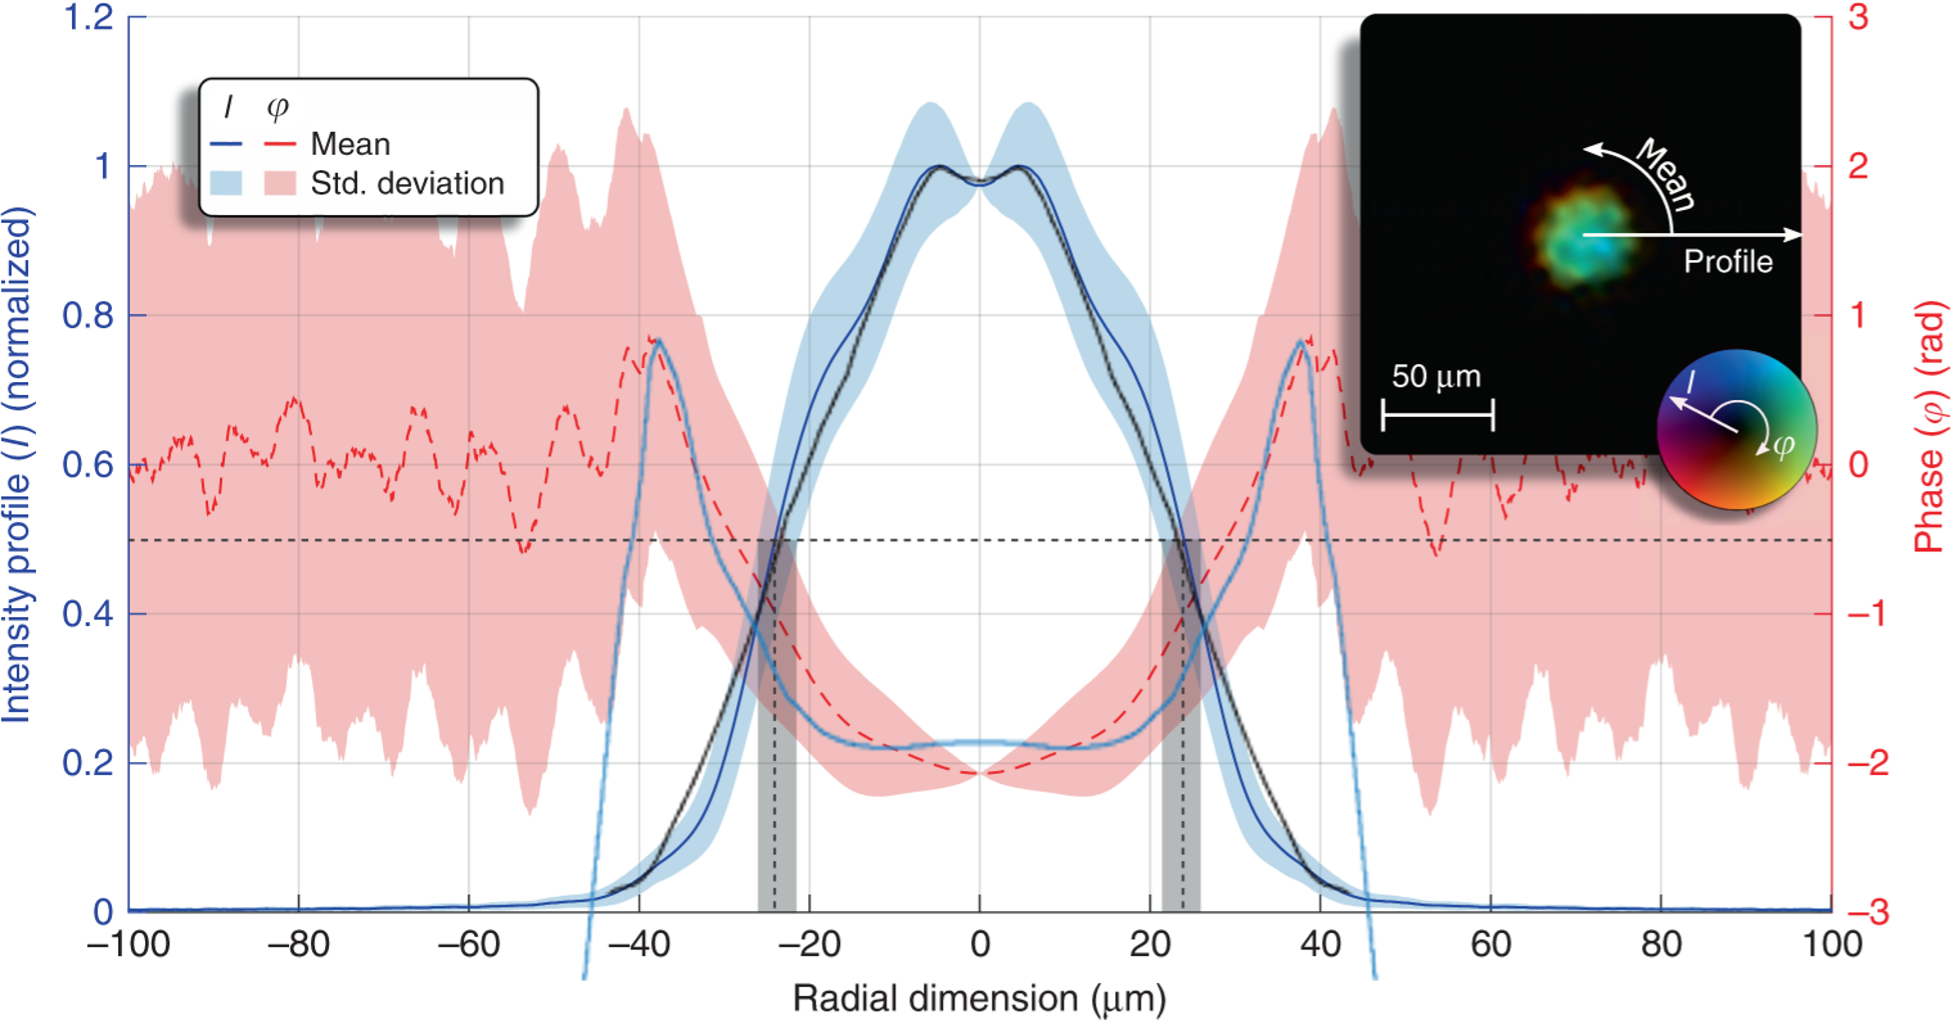
\includegraphics[width=0.75\textwidth]{Figuras/ch4_cmp72.png}
  \caption{Comparación entre los perfiles radiales de intensidad--fase con $r_{u}=\qty{15}{µm}$, manteniendo los valores de los parámetros $r_{L}=\qty{5}{µm}$, $\sigma_{L}=\qty{15}{µm}$ y $\sigma_{u}=\qty{17}{µm}$; y el experimento.}
  \label{fig:4.31}
\end{figure}

\begin{table}[htpb]
  \centering
  \scriptsize
  \caption{Parámetros utilizados en las simulaciones con función exponencial por tramos, variando $r_{u}$ (en azul) entre \qty{10}{µm} y \qty{15}{µm}. El símbolo del \enquote{tick} señala las simulaciones con buen acuerdo.}
  \label{tab:4.9}
  \begin{tabular}{S>{\color{miazul}}SSSSSSSSS}
  \toprule
  {$r_{L}$ (\unit{\um})} & {$r_{u}$ (\unit{\um})} & {$\sigma_{L}$ (\unit{\um})} & {$\sigma_{u}$ (\unit{\um})} & {\texttt{zshift}} & {\texttt{cen\_fac}} & {$\sigma_{z0}$ (\unit{mm})} & {$\sigma_{r0}$ (\unit{\um})} & {$z_{ion,1}$ (\unit{mm})} & {$z_{ion,2}$ (\unit{mm})} \\ 
  \midrule
  5  & 10  & 15 & 17  & 0.75  & 0.075  & 2  & 15  & 0  & 3.75  \\
  5  & 15  & 15 & 17  & 0.75  & 0.075  & 2  & 15  & 0  & 3.75  \\
  5  & 18  & 15 & 17  & 0.75  & 0.075  & 2  & 15  & 0  & 3.75  \\
  5  & 20  & 15 & 17  & 0.75  & 0.075  & 2  & 15  & 0  & 3.75  \\
  \bottomrule
  \end{tabular}
\end{table}

\subsection{Variando el parámetro \texorpdfstring{$\sigma_{u}$}{sigma-u}}\label{sec:4.3.2}
Los efectos de la desviación típica $\sigma_{u}$ pueden resumirse en un rápido ensanchamiento del perfil de intensidad ensanchamiento, hasta deformar completamente la mitad inferior o falda de la curva, a medida que aumenta este parámetro desde $\sigma_{u}=\qty{17}{µm}$ hasta $\sigma_{u}=\qty{25}{µm}$, pasando por $\sigma_{u}=\qty{20}{µm}$, recogidos en la Tabla \ref{tab:4.10}. Ninguna de estas tres simulaciones presentan un buen acuerdo, pues el parámetro $r_{u}=\qty{18}{µm}$ fijado ubica la transición de la pendiente para radios demasiado elevados, no consiguiéndose el resultado preciso del ancho de la falda.

\begin{figure}[htbp]
  \centering
  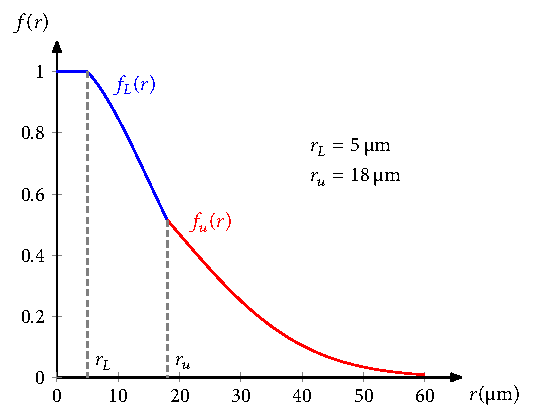
\includegraphics[width=0.45\textwidth]{Figuras/ch4_fexp2.pdf}
  \caption{Función exponencial con $\sigma_{u}=\qty{20}{µm}$, manteniendo los valores de los parámetros $r_{L}=\qty{5}{µm}$, $r_{u}=\qty{18}{µm}$ y $\sigma_{L}=\qty{15}{µm}$.}
  \label{fig:4.32}
\end{figure}

Cuando la función exponencial empleada viene dada gráficamente por la Figura \ref{fig:4.32}, los resultados observados presentan una mayor profundidad en la fase, mostrados en la Figura \ref{fig:4.33}.

\begin{figure}[htbp]
  \centering
  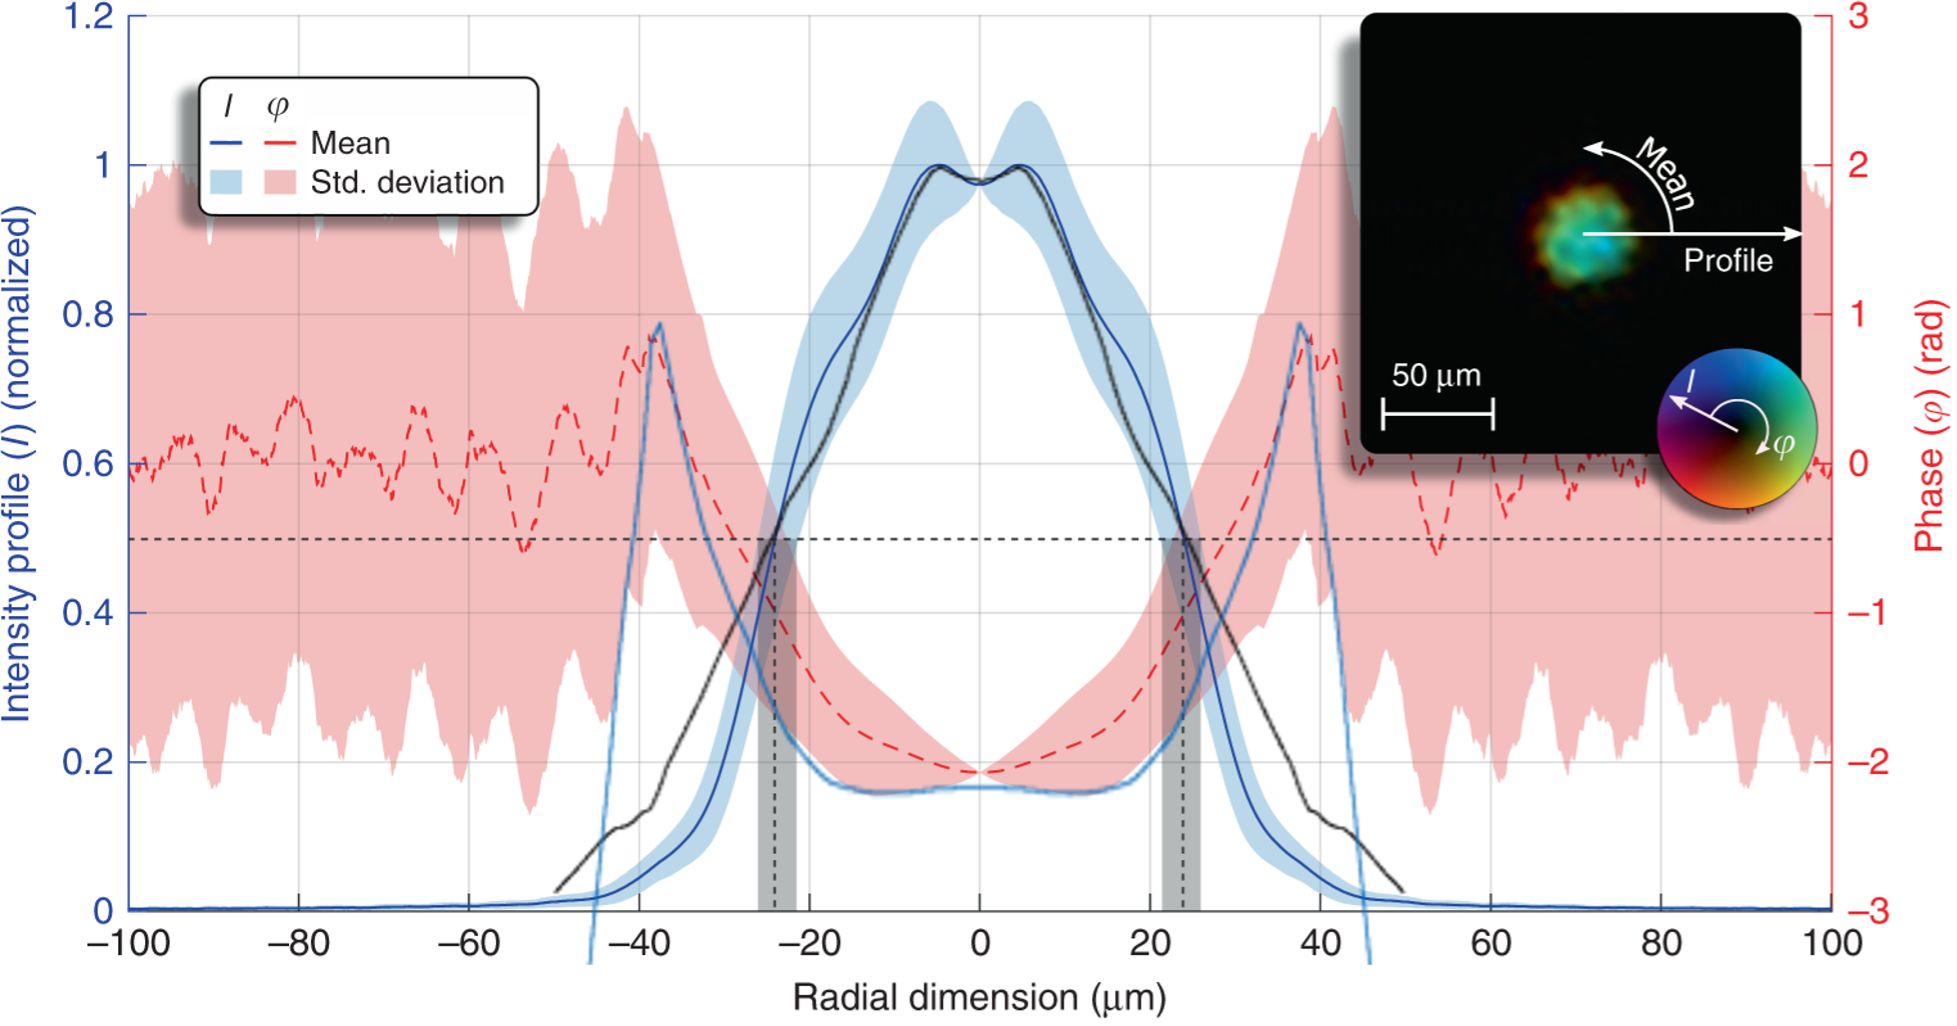
\includegraphics[width=0.7\textwidth]{Figuras/ch4_cmp81.png}
  \caption{Comparación entre los perfiles radiales de intensidad--fase con $\sigma_{u}=\qty{20}{µm}$, manteniendo los valores de los parámetros $r_{L}=\qty{5}{µm}$, $\sigma_{L}=\qty{15}{µm}$ y $r_{u}=\qty{18}{µm}$; y el experimento.}
  \label{fig:4.33}
\end{figure}

\begin{table}[htpb]
  \centering
  \scriptsize
  \caption{Parámetros utilizados en las simulaciones con función exponencial por tramos, variando $\sigma_{u}$ (en azul) entre \qty{17}{µm} y \qty{25}{µm}. El símbolo del \enquote{tick} señala las simulaciones con buen acuerdo.}
  \label{tab:4.10}
  \begin{tabular}{SSS>{\color{miazul}}SSSSSSS}
  \toprule
  {$r_{L}$ (\unit{\um})} & {$r_{u}$ (\unit{\um})} & {$\sigma_{L}$ (\unit{\um})} & {$\sigma_{u}$ (\unit{\um})} & {\texttt{zshift}} & {\texttt{cen\_fac}} & {$\sigma_{z0}$ (\unit{mm})} & {$\sigma_{r0}$ (\unit{\um})} & {$z_{ion,1}$ (\unit{mm})} & {$z_{ion,2}$ (\unit{mm})} \\ 
  \midrule
  5  & 18  & 15 & 17  & 0.75  & 0.075  & 2  & 15  & 0  & 3.75  \\
  5  & 18  & 15 & 20  & 0.75  & 0.075  & 2  & 15  & 0  & 3.75  \\
  5  & 18  & 15 & 25  & 0.75  & 0.075  & 2  & 15  & 0  & 3.75  \\
  \bottomrule
  \end{tabular}
\end{table}

\subsection{Introduciendo \acrshort{oam}}\label{sec:4.3.3}
Aprovechando los resultados numéricos obtenidos en la sección \S\ref{sec:4.3.1}, entre los que estaba la primera simulación con mejor ajuste experimental (cuando $r_{u}=\qty{10}{µm}$, $r_{L}=\qty{5}{µm}$, $\sigma_{L}=\qty{15}{µm}$ y $\sigma_{u}=\qty{17}{µm}$), llega el momento para cambiar la perspectiva inicial de las simulaciones añadiendo el \acrshort{oam} en la semilla \acrshort{hoh}.

En detalle, el haz gaussiano inicial es sustituido por un haz de Laguerre-Gauss con índices $p=0$ y $l=25$, manteniendo la función exponencial para controlar la región de abundancia de \ce{Kr^{8+}} dentro del canal de plasma. La activación del modo de Laguerre-Gauss requiere la habilitación en los datos iniciales alimentados en Dagon (vistos en la Tabla \ref{tab:3.1}) de los parámetros \texttt{fwhmx} y \texttt{fwhmy}. Iniciando las simulaciones, los valores $\texttt{fwhm}=\texttt{fwhmx}=\texttt{fwhmy}=\qty{25}{µm}$ encabezan el primer grupo, manteniendo los demás parámetros ya comentados constantes.

Las Figuras \ref{fig:ch4_oam1} y \ref{fig:ch4_oam2} presentan una distribución fuertemente contaminada por un ruido que distorsiona gravemente la forma de ambos perfiles. En principio, es complicado determinar cuál es el fenómeno responsable de este comportamiento, por lo que es necesario recurrir al programa VisIt para obtener otras perspectivas que resuelvan la incógnita. De este modo, las Figuras \ref{fig:ch4_oam3} y \ref{fig:ch4_oam4} extraídas con VisIt muestran la curva de intensidad de la semilla en secciones transversales del canal según los ejes $XZ$ e $YZ$, respectivamente.

\begin{figure}[htbp]
  \centering
  \begin{subcaptionblock}{.4\textwidth}
    \centering
    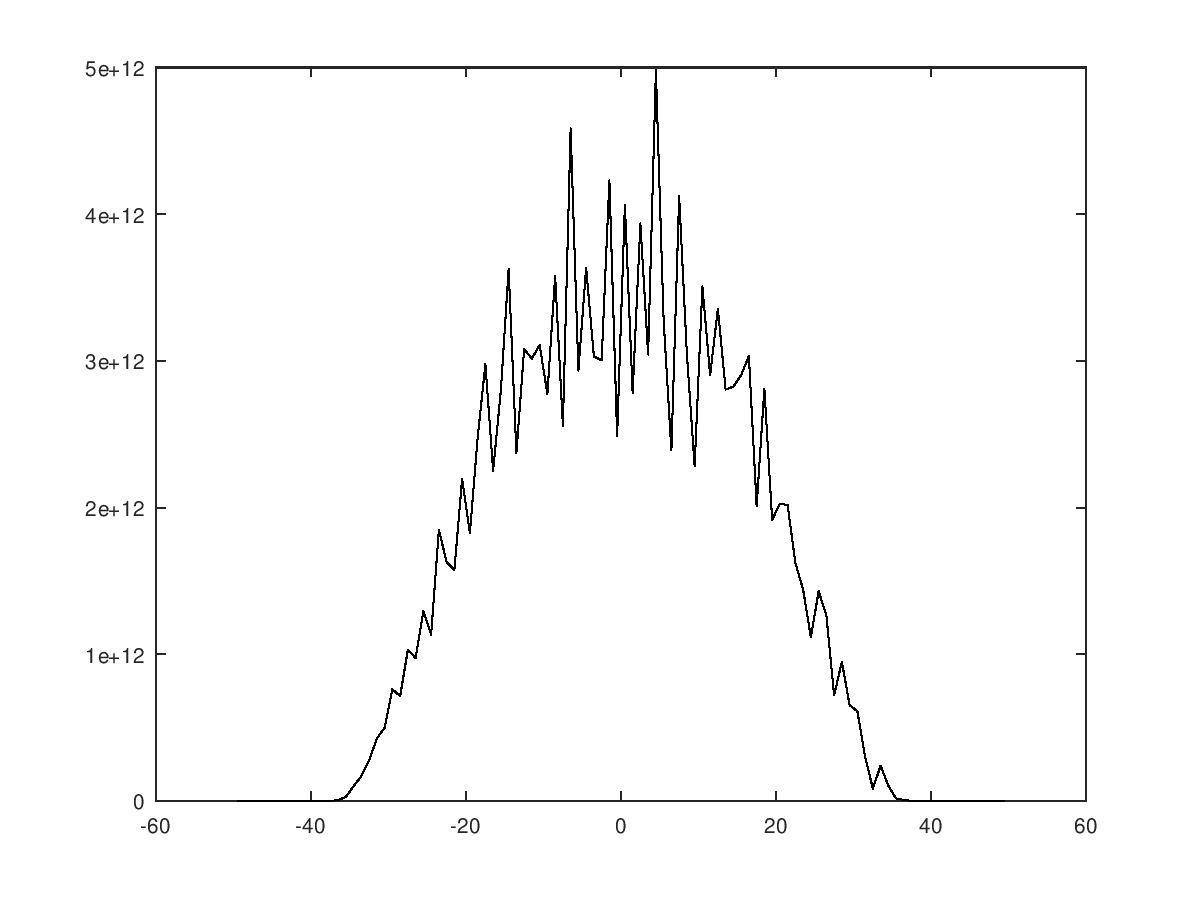
\includegraphics[width=\textwidth]{Figuras/ch4_oam1.png}
    \caption{Perfil radial de intensidad (\unit{W/cm^2}) frente al radio (\unit{µm})}\label{fig:ch4_oam1}
  \end{subcaptionblock}
  \begin{subcaptionblock}{.4\textwidth}
    \centering
    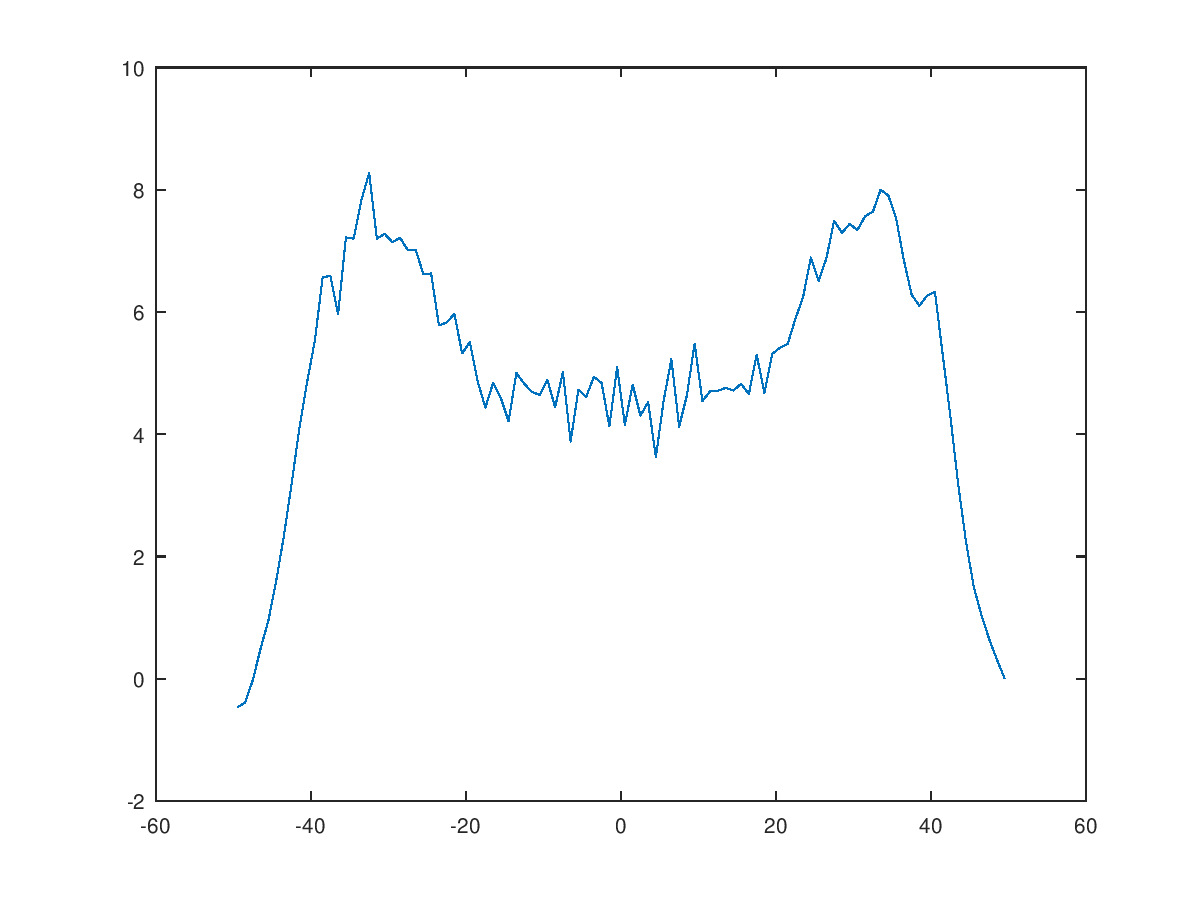
\includegraphics[width=\textwidth]{Figuras/ch4_oam2.png}
    \caption{Perfil radial de fase (\unit{rad}) frente al radio (\unit{µm})}\label{fig:ch4_oam2}
  \end{subcaptionblock}
   \caption{Distribución radial de intensidad--fase para un haz de Laguerre--Gauss con $p=0$, $l=25$ y $\texttt{fwhm}=\qty{25}{µm}$; manteniendo $r_{L}=\qty{5}{µm}$, $r_{u}=\qty{15}{µm}$, $\sigma_{L}=\qty{15}{µm}$ y $\sigma_{u}=\qty{17}{µm}$.}
   \label{fig:4.34}
\end{figure}

A partir de estas imágenes, puede concluirse que el perfil de intensidad del pulso está asociado a una distribución con forma de gaussiana mezclada con un fondo aleatorio, responsable del ruido estocástico. Este tipo de fenómeno está asociado con la amplificación de la emisión espontánea (\acrshort{ase}) de la radiación, debido principalmente a que la emisión espontánea de los fotones es intrínsecamente estocástica, otorgándole a los perfiles el ruido característico.

También es posible emplear VisIt para extraer secciones transversales de la intensidad y la fase de los fotones en el haz de Laguerre-Gauss. En las Figuras \ref{fig:ch4_oam5} y \ref{fig:ch4_oam6} se muestran la intensidad y la fase en el plano $XY$ de la columna de plasma, cuando la intensidad alcanzada en $z=\qty{4.735}{mm}$ es máxima.

\begin{figure}[htbp]
  \centering
  \begin{subcaptionblock}{.4\textwidth}
    \centering
    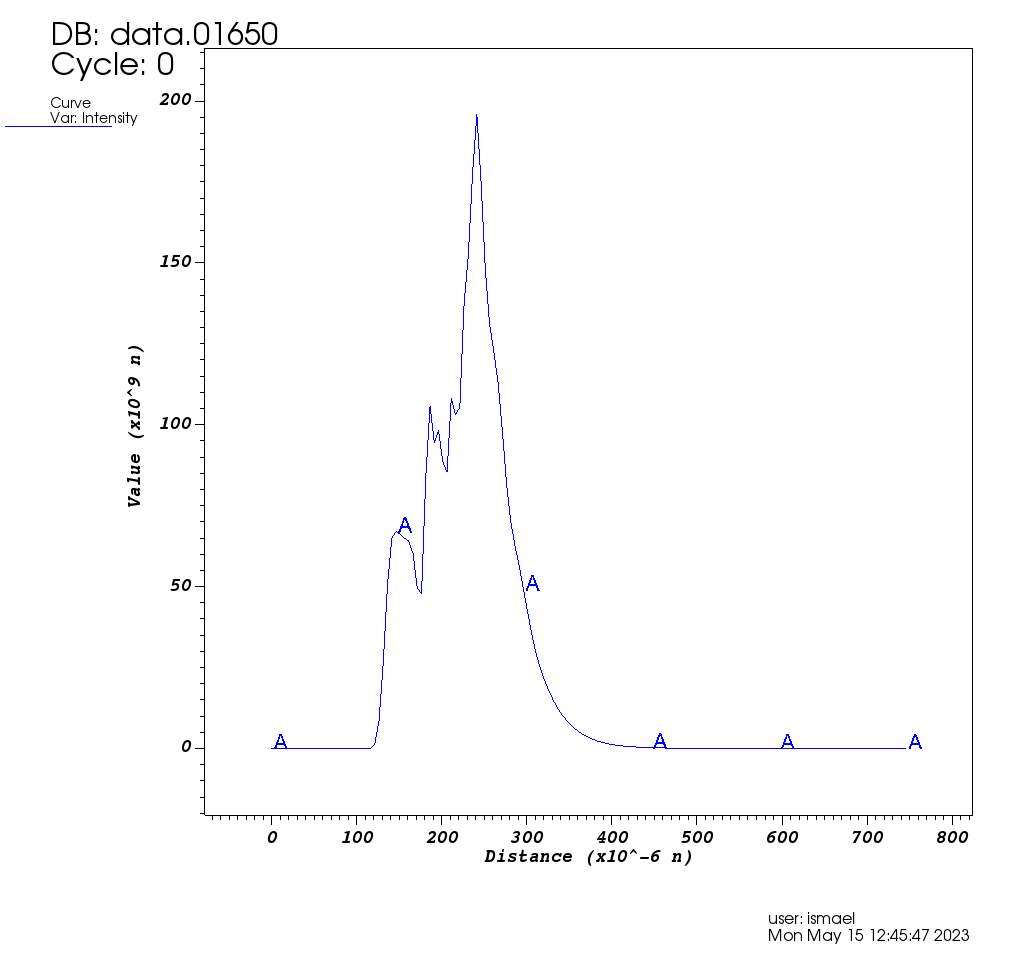
\includegraphics[width=0.9\textwidth]{Figuras/ch4_oam3.png}
    \caption{Perfil de intensidad en el plano $XZ$}\label{fig:ch4_oam3}
  \end{subcaptionblock}
  \begin{subcaptionblock}{.4\textwidth}
    \centering
    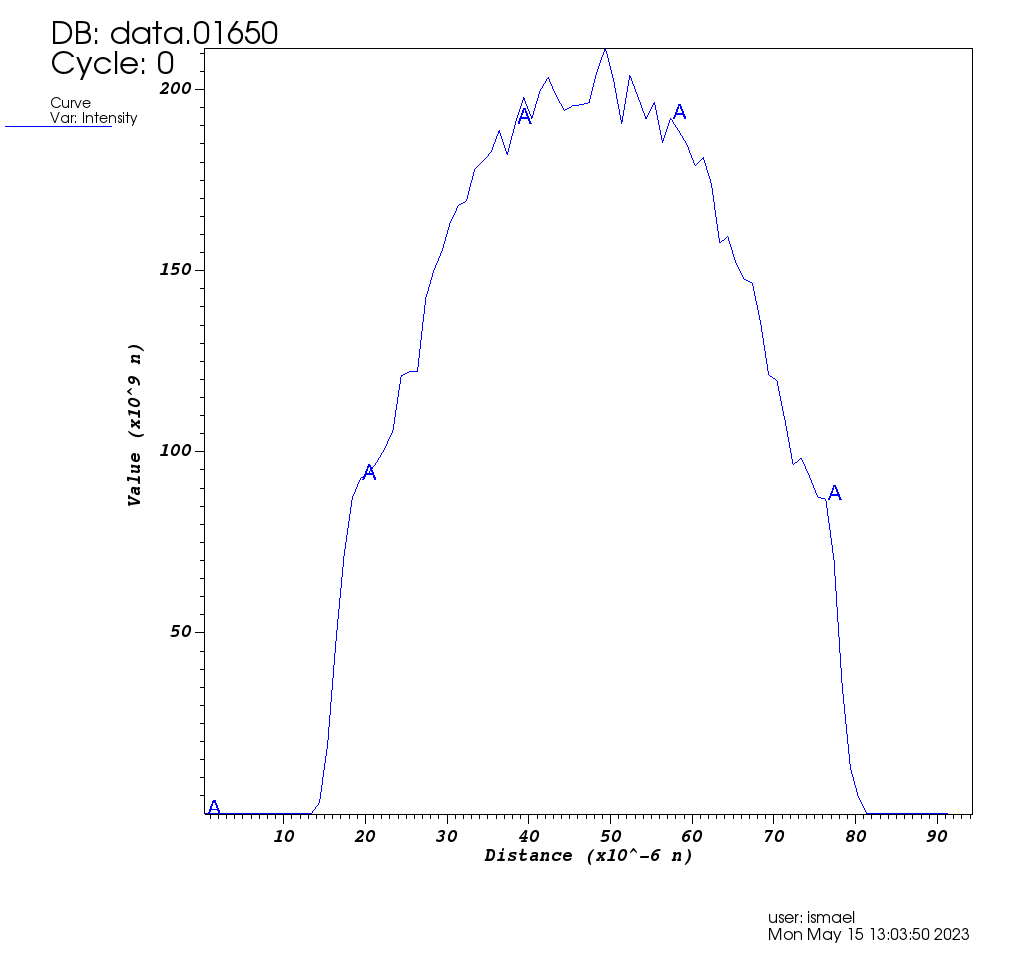
\includegraphics[width=0.9\textwidth]{Figuras/ch4_oam4.png}
    \caption{Perfil de intensidad en el plano $YZ$}\label{fig:ch4_oam4}
  \end{subcaptionblock}
   \caption{Perfiles de intensidad del pulso de Laguerre-Gauss con $p=0$, $l=25$ y $\texttt{fwhm}=\qty{25}{µm}$; manteniendo $r_{L}=\qty{5}{µm}$, $r_{u}=\qty{15}{µm}$, $\sigma_{L}=\qty{15}{µm}$ y $\sigma_{u}=\qty{17}{µm}$.}
   \label{fig:4.35}
\end{figure}

Estas imágenes demuestran algunas de las características típicas del haz de Laguerre-Gauss y también confirman algunas sospechas sobre el \acrshort{ase}. La sección transversal de intensidad está restringida a una región circular de \qty{30}{µm}, con un máximo global centrado en dicha región, atribuible exclusivamente entonces la amplificación en la zona al \acrshort{ase}, y no a la amplificación de la propia semilla \acrshort{hoh}. 

Por otra parte, la fase está formada por un anillo rodeado de $25$ líneas rectas alabeadas. El número de línea viene determinado por la magnitud de la carga topológica $l=25$, mientras que la curvatura adquirida por las líneas es una desviación respecto de los segmentos rectos que deberían aparecer. Teniendo en cuenta que se trata de la fase de los fotones amplificados, esta discrepancia está relacionada con la densidad electrónica del canal, debida a gradientes de densidad electrónica pronunciados.

\begin{figure}[htbp]
  \centering
  \begin{subcaptionblock}{.4\textwidth}
    \centering
    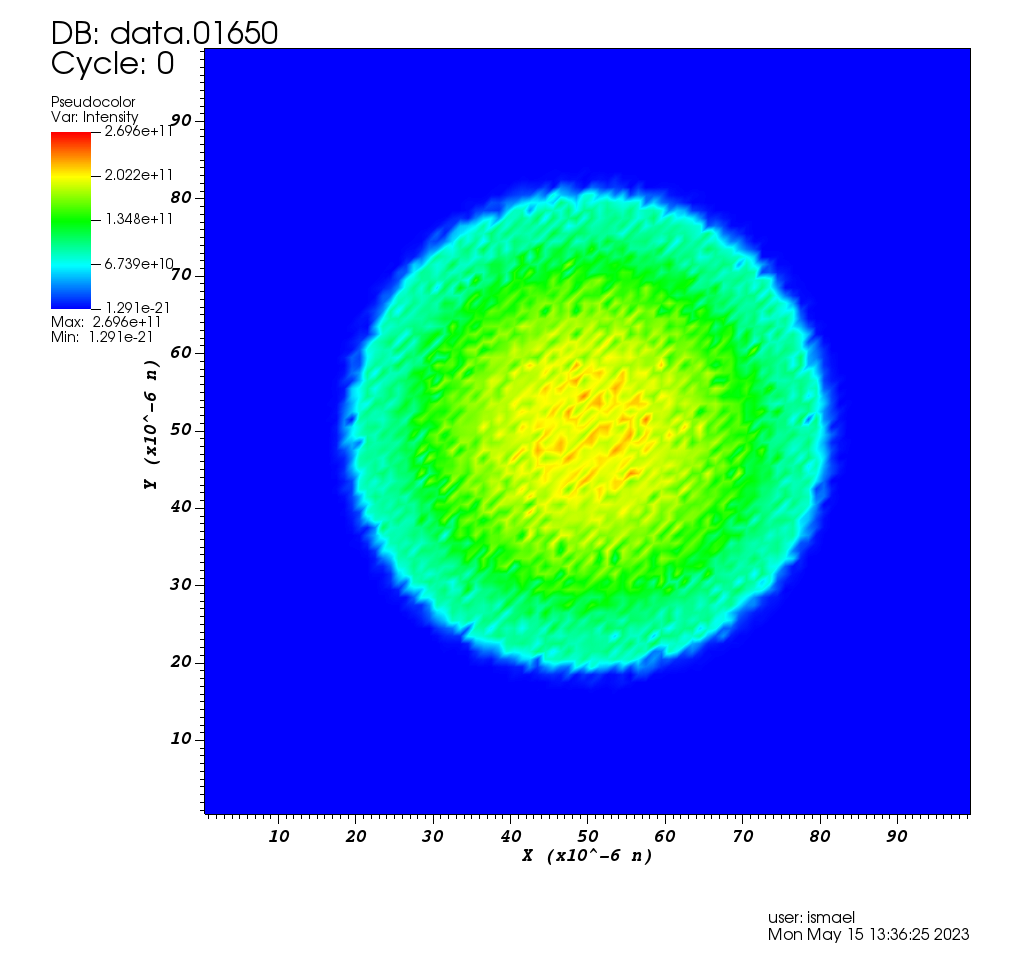
\includegraphics[width=\textwidth]{Figuras/ch4_oam5.png}
    \caption{Sección transversal de intensidad en el plano $XY$}\label{fig:ch4_oam5}
  \end{subcaptionblock}
  \begin{subcaptionblock}{.4\textwidth}
    \centering
    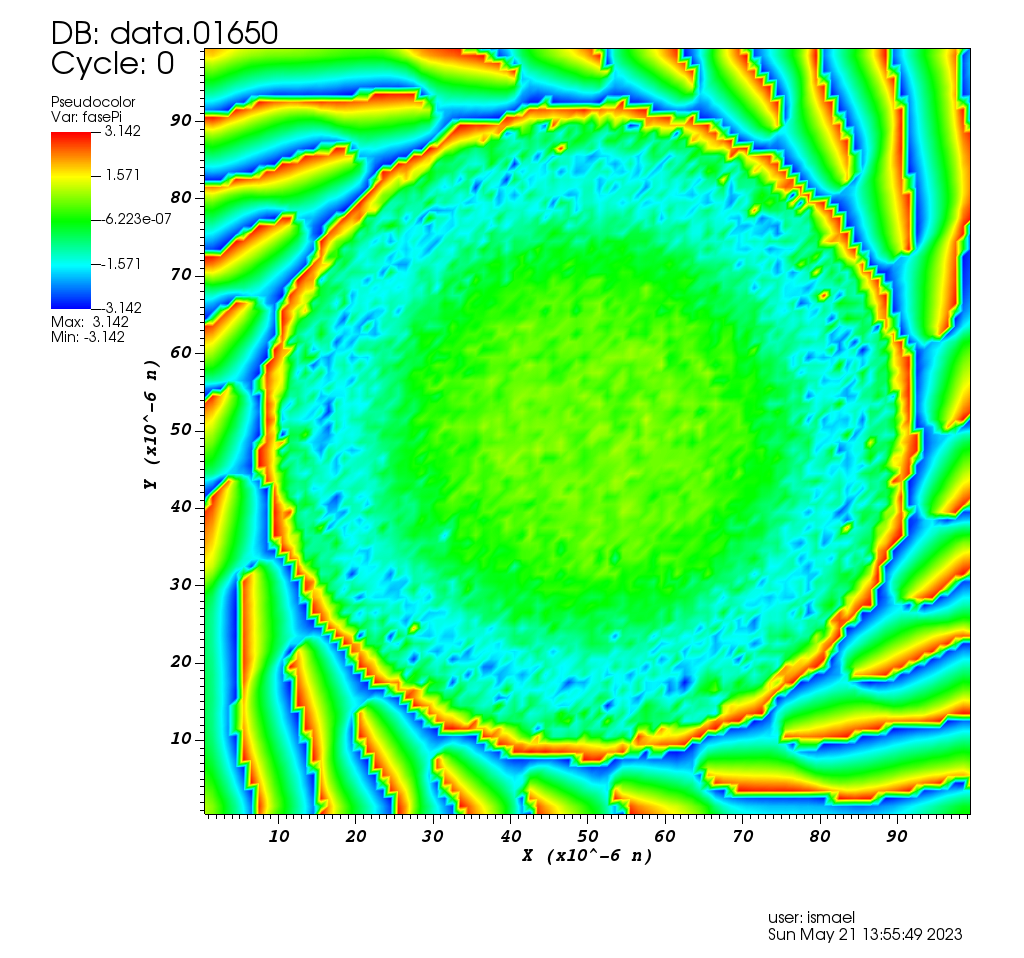
\includegraphics[width=\textwidth]{Figuras/ch4_oam6.png}
    \caption{Sección transversal de fase en el plano $XY$}\label{fig:ch4_oam6}
  \end{subcaptionblock}
   \caption{Secciones transversales de intensidad--fase del pulso de Laguerre-Gauss con $p=0$, $l=25$ y $\texttt{fwhm}=\qty{25}{µm}$; manteniendo $r_{L}=\qty{5}{µm}$, $r_{u}=\qty{15}{µm}$, $\sigma_{L}=\qty{15}{µm}$ y $\sigma_{u}=\qty{17}{µm}$.}
   \label{fig:4.36}
\end{figure}

Siguiendo con los resultados de intensidad y fase obtenidos, el último paso ejecutado consiste en incrementar el parámetro para la amplitud del pulso \texttt{fwhm}, duplicando el valor inicial empleado. En esta situación, $\texttt{fwhm}=\texttt{fwhmx}=\texttt{fwhmy}=\qty{50}{µm}$, y los demás parámetros relativos a la columna de plasma permanecen constantes. Para sintetizar estos últimos resultados, se presenta el único caso especial donde, en contra de lo esperado y de forma sorprendente, desaparecen los perfiles estocásticos en intensidad y fase.

Las Figuras \ref{fig:ch4_oam7} y \ref{fig:ch4_oam8} muestran los perfiles conseguidos cuando el radio de la transición entre los tramos de la función exponencial es $r_{u}=\qty{20}{µm}$. Sin duda se trata de un suceso extraño, porque el único parámetro responsable de conseguir amplificar la semilla \acrshort{hoh} parece ser $r_{u}=\qty{20}{µm}$, pues las otras simulaciones (ver el anexo \S\ref{anx:3}) difieren únicamente en el valor de ese parámetro. Por el contrario, las Figuras \ref{fig:ch4_oam7u} y \ref{fig:ch4_oam8u} presentan el mismo fondo estocástico observado anteriormente cuando $\texttt{fwhm}=\qty{25}{µm}$.

¿Por qué el radio $r_{u}=\qty{20}{µm}$ marca la diferencia entre el dominio del \acrshort{ase} frente al dominio de la amplificación del haz de Laguerre-Gauss? Las secciones transversales en $XY$ de intensidad y fase, representadas en las Figuras \ref{fig:ch4_oam9} y \ref{fig:ch4_oam10}, presentan el comportamiento esperable del modo de Laguerre-Gauss, siendo necesario arrojar más luz sobre este asunto en futuros estudios. Una posible propuesta consiste en asociar el dominio de la amplificación estimulada de la semilla con una región de abundancia de \ce{Kr^{8+}} suficientemente amplia, acompañada por densidades electrónicas con una distribución que favorezcan la inversión de población.

\begin{figure}[htbp]
  \centering
  \begin{subcaptionblock}{.4\textwidth}
    \centering
    \includegraphics[width=\textwidth]{Figuras/ch4_oam7.png}
    \caption{Perfil radial de intensidad (\unit{W/cm^2}) frente al radio (\unit{µm})}\label{fig:ch4_oam7}
  \end{subcaptionblock}
  \begin{subcaptionblock}{.4\textwidth}
    \centering
    \includegraphics[width=\textwidth]{Figuras/ch4_oam8.png}
    \caption{Perfil radial de fase (\unit{rad}) frente al radio (\unit{µm})}\label{fig:ch4_oam8}
  \end{subcaptionblock}
   \caption{Distribución radial de intensidad--fase para un haz de Laguerre--Gauss con $p=0$, $l=25$ y $\texttt{fwhm}=\qty{50}{µm}$; manteniendo $r_{L}=\qty{5}{µm}$, $r_{u}=\qty{20}{µm}$, $\sigma_{L}=\qty{15}{µm}$ y $\sigma_{u}=\qty{17}{µm}$.}
   \label{fig:4.37}
\end{figure}

\begin{figure}[htbp]
  \centering
  \begin{subcaptionblock}{.4\textwidth}
    \centering
    \includegraphics[width=\textwidth]{Figuras/ch4_oam7u.png}
    \caption{Perfil radial de intensidad (\unit{W/cm^2}) frente al radio (\unit{µm})}\label{fig:ch4_oam7u}
  \end{subcaptionblock}
  \begin{subcaptionblock}{.4\textwidth}
    \centering
    \includegraphics[width=\textwidth]{Figuras/ch4_oam8u.png}
    \caption{Perfil radial de fase (\unit{rad}) frente al radio (\unit{µm})}\label{fig:ch4_oam8u}
  \end{subcaptionblock}
   \caption{Distribución radial de intensidad--fase para un haz de Laguerre--Gauss con $p=0$, $l=25$ y $\texttt{fwhm}=\qty{50}{µm}$; manteniendo $r_{L}=\qty{5}{µm}$, $r_{u}=\qty{18}{µm}$, $\sigma_{L}=\qty{15}{µm}$ y $\sigma_{u}=\qty{17}{µm}$.}
   \label{fig:4.37}
\end{figure}

\begin{figure}[htbp]
  \centering
  \begin{subcaptionblock}{.4\textwidth}
    \centering
    \includegraphics[width=\textwidth]{Figuras/ch4_oam9.png}
    \caption{Sección transversal de intensidad en el plano $XY$}\label{fig:ch4_oam9}
  \end{subcaptionblock}
  \begin{subcaptionblock}{.4\textwidth}
    \centering
    \includegraphics[width=\textwidth]{Figuras/ch4_oam10.png}
    \caption{Sección transversal de fase en el plano $XY$}\label{fig:ch4_oam10}
  \end{subcaptionblock}
   \caption{Secciones transversales de intensidad--fase del pulso de Laguerre-Gauss con $p=0$, $l=25$ y $\texttt{fwhm}=\qty{50}{µm}$; manteniendo $r_{L}=\qty{5}{µm}$, $r_{u}=\qty{20}{µm}$, $\sigma_{L}=\qty{15}{µm}$ y $\sigma_{u}=\qty{17}{µm}$.}
   \label{fig:4.38}
\end{figure}

En cualquier caso, aunque la inyección de \acrshort{oam} es muy interesante por variedad de fenómenos físicos que aparecen, el ajuste conseguido al añadir esta propiedad óptica ha empeorado los resultados conseguidos durante la sección \S\ref{sec:4.3.2}, donde todavía no había sido introducida la figura del haz de Laguerre--Gauss. El ruido estocástico de la \acrshort{ase} introducida en las distribuciones gaussianas enmascara la acción de las funciones destinadas a controlar estos perfiles.

\subsection{Eliminando \acrshort{ase}}\label{sec:4.3.4}
A raíz de las observaciones realizadas en la sección \S\ref{sec:4.3.3}, para confirmar con mayor seguridad los efectos de la \acrshort{ase} en la amplificación del pulso, es posible eliminar manualmente en Dagon la amplificación de la emisión espontánea, siendo así capaces de conocer con mayor precisión los efectos sobre los perfiles radiales de intensidad y fase.

Anulando la \acrshort{ase}, las Figuras \ref{fig:ch4_ase1} y \ref{fig:ch4_ase2} muestran los resultados sin \acrshort{ase} de las simulaciones, manteniendo los parámetros de la columna de plasma utilizados anteriormente. El perfil radial de intensidad presenta un pozo donde debería estar el valle de sobreionización inicial, señal evidente de que la intensidad en esa región es debida prácticamente en su totalidad a los efectos de la \acrshort{ase}, mientras que la amplificación del haz de Laguerre-Gauss contribuye para radios mayores del canal. El perfil de fase aparece completamente deformado, revelando una conexión entre la \acrshort{ase} y la distribución de electrones en el canal.

\begin{figure}[htbp]
  \centering
  \begin{subcaptionblock}{.4\textwidth}
    \centering
    \includegraphics[width=\textwidth]{Figuras/ch4_int_ase.png}
    \caption{Perfil radial de intensidad (\unit{W/cm^2}) frente al radio (\unit{µm})}\label{fig:ch4_ase1}
  \end{subcaptionblock}
  \begin{subcaptionblock}{.4\textwidth}
    \centering
    \includegraphics[width=\textwidth]{Figuras/ch4_fs_ase.png}
    \caption{Perfil radial de fase (\unit{rad}) frente al radio (\unit{µm})}\label{fig:ch4_ase2}
  \end{subcaptionblock}
   \caption{Distribución radial de intensidad--fase para un haz de Laguerre--Gauss con $p=0$, $l=25$ y $\texttt{fwhm}=\qty{25}{µm}$; manteniendo $r_{L}=\qty{5}{µm}$, $r_{u}=\qty{20}{µm}$, $\sigma_{L}=\qty{15}{µm}$ y $\sigma_{u}=\qty{17}{µm}$.}
   \label{fig:4.39}
\end{figure}

Las secciones transversales en el plano $XY$ de intensidad y fase, en las Figuras \ref{fig:ch4_ase3} y \ref{fig:ch4_ase4}, confirman la apariencia de los perfiles. La zona central del anillo tiene intensidad nula, delimitando una región con un radio de \qty{10}{µm}, mientras que el perfil alabeado de la fase, y el número de anillos alternantes entre $-\pi$ y $\pi$ proporcionan información a cerca del modo inyectado.

\begin{figure}[htbp]
  \centering
  \begin{subcaptionblock}{.4\textwidth}
    \centering
    \includegraphics[width=\textwidth]{Figuras/ch4_ase1.png}
    \caption{Sección transversal de intensidad en el plano $XY$}\label{fig:ch4_ase3}
  \end{subcaptionblock}
  \begin{subcaptionblock}{.4\textwidth}
    \centering
    \includegraphics[width=\textwidth]{Figuras/ch4_ase2.png}
    \caption{Sección transversal de fase en el plano $XY$}\label{fig:ch4_ase4}
  \end{subcaptionblock}
   \caption{Secciones transversales de intensidad--fase del pulso de Laguerre-Gauss con $p=0$, $l=25$ y $\texttt{fwhm}=\qty{25}{µm}$; manteniendo $r_{L}=\qty{5}{µm}$, $r_{u}=\qty{20}{µm}$, $\sigma_{L}=\qty{15}{µm}$ y $\sigma_{u}=\qty{17}{µm}$.}
   \label{fig:4.39}
\end{figure}
